\documentclass[compress]{beamer}
\mode<presentation>
\setbeamercovered{transparent}
\usetheme{Warsaw}
%\useoutertheme{smoothtree}
\usepackage{multirow}
\usepackage[english]{babel}
\usepackage[latin1]{inputenc}
\usepackage{times}
\usepackage[T1]{fontenc}
\usepackage{xmpmulti}
\usepackage{multicol}
\usepackage{colortbl}
%\setbeamersize{text margin left=.25 in,text margin right=.25 in}
\setbeamersize{text margin left=.15 in,text margin right=.15 in}
\usepackage[authoryear]{natbib}
\usepackage{epstopdf}
\definecolor{antiquebrass}{rgb}{0.8, 0.58, 0.46}
\definecolor{babyblueeyes}{rgb}{0.63, 0.79, 0.95}
\definecolor{babyblue}{rgb}{0.54, 0.81, 0.94}
\definecolor{bistre}{rgb}{0.24, 0.17, 0.12}
\definecolor{brightlavender}{rgb}{0.75, 0.58, 0.89}
\definecolor{bulgarianrose}{rgb}{0.28, 0.02, 0.03}
\definecolor{slateblue}{rgb}{0.56, 0.74, 0.56}
\definecolor{cordovan}{rgb}{0.54, 0.25, 0.27}
\definecolor{darkbyzantium}{rgb}{0.36, 0.22, 0.33}
\setbeamercolor{structure}{fg=cordovan!70, bg= black!60}
\usepackage{tikz}
\usetikzlibrary{shadows,calc}
\usetikzlibrary{shadows.blur}
\usetikzlibrary{shapes.symbols}
\usepackage{hyperref}
\usepackage{booktabs}
\usepackage{colortbl}
\usepackage{multirow}
%%%%%%%%% shaddow image %%%%%
% some parameters for customization
\def\shadowshift{3pt,-3pt}
\def\shadowradius{6pt}
\colorlet{innercolor}{black!60}
\colorlet{outercolor}{gray!05}
% this draws a shadow under a rectangle node
\newcommand\drawshadow[1]{
\begin{pgfonlayer}{shadow}
    \shade[outercolor,inner color=innercolor,outer color=outercolor] ($(#1.south west)+(\shadowshift)+(\shadowradius/2,\shadowradius/2)$) circle (\shadowradius);
    \shade[outercolor,inner color=innercolor,outer color=outercolor] ($(#1.north west)+(\shadowshift)+(\shadowradius/2,-\shadowradius/2)$) circle (\shadowradius);
    \shade[outercolor,inner color=innercolor,outer color=outercolor] ($(#1.south east)+(\shadowshift)+(-\shadowradius/2,\shadowradius/2)$) circle (\shadowradius);
    \shade[outercolor,inner color=innercolor,outer color=outercolor] ($(#1.north east)+(\shadowshift)+(-\shadowradius/2,-\shadowradius/2)$) circle (\shadowradius);
    \shade[top color=innercolor,bottom color=outercolor] ($(#1.south west)+(\shadowshift)+(\shadowradius/2,-\shadowradius/2)$) rectangle ($(#1.south east)+(\shadowshift)+(-\shadowradius/2,\shadowradius/2)$);
    \shade[left color=innercolor,right color=outercolor] ($(#1.south east)+(\shadowshift)+(-\shadowradius/2,\shadowradius/2)$) rectangle ($(#1.north east)+(\shadowshift)+(\shadowradius/2,-\shadowradius/2)$);
    \shade[bottom color=innercolor,top color=outercolor] ($(#1.north west)+(\shadowshift)+(\shadowradius/2,-\shadowradius/2)$) rectangle ($(#1.north east)+(\shadowshift)+(-\shadowradius/2,\shadowradius/2)$);
    \shade[outercolor,right color=innercolor,left color=outercolor] ($(#1.south west)+(\shadowshift)+(-\shadowradius/2,\shadowradius/2)$) rectangle ($(#1.north west)+(\shadowshift)+(\shadowradius/2,-\shadowradius/2)$);
    \shade[outercolor,right color=innercolor,left color=innercolor] ($(#1.north west)+(-\shadowradius/12,\shadowradius/12)$) rectangle ($(#1.south east)+(\shadowradius/12,-\shadowradius/12)$);%Frame
    \filldraw ($(#1.south west)+(\shadowshift)+(\shadowradius/2,\shadowradius/2)$) rectangle ($(#1.north east)+(\shadowshift)-(\shadowradius/2,\shadowradius/2)$);
\end{pgfonlayer}
}
% create a shadow layer, so that we don't need to worry about overdrawing other things
\pgfdeclarelayer{shadow} 
\pgfsetlayers{shadow,main}
% Define image shadow command
\newcommand\shadowimage[2][]{%
\begin{tikzpicture}
\node[anchor=south west,inner sep=0] (image) at (0,0) {\includegraphics[#1]{#2}};
\drawshadow{image}
\end{tikzpicture}}
\usepackage{calligra}

\DeclareMathOperator*{\argmax}{Arg\,max}
\DeclareMathOperator*{\argmin}{Arg\,min}
\newcommand{\norm}[1]{\left\Vert #1 \right\Vert }
\newcommand{\bbetaHat}{ \widehat{\bbeta}}
\newcommand{\bbetaLSE}{ \widehat{\bbeta}_{_{\text{LSE}}}}
\newcommand{\bbetaMLE}{ \widehat{\bbeta}_{_{\text{MLE}}}}
\newcommand{\sqBullet}[1]{  {\tiny \tiny \tiny \qBoxCol{#1!60}{ }} }
%***************
%\newtheorem{thm}{Theorem}
%\documentclass[noinfoline]{imsart}
%\usepackage{amsmath,amstext,amssymb}
%%\usepackage[top=1.5in, bottom=1.5in, left=1.2in, right=1.2in]{geometry}
%% settings
%%\pubyear{2005}
%%\volume{0}
%%\issue{0}
%%\firstpage{1}
%%\lastpage{8}
%\arxiv{arXiv:0000.0000}

%\startlocaldefs
%\numberwithin{equation}{section}
%\theoremstyle{plain}
%\newtheorem{thm}{Theorem}
%\endlocaldefs
\usepackage{lipsum} 
\usepackage{amsmath}
\usepackage{amssymb}
\usepackage{amsbsy} 
\usepackage{amsthm}
\usepackage{mathrsfs}
\usepackage{eufrak}
\usepackage{mathrsfs}
\usepackage{color}
\usepackage{verbatim}
\usepackage{graphicx}
\usepackage{bm}
\usepackage{enumerate}
\usepackage{epstopdf} 
\usepackage{natbib}
\usepackage{undertilde}
%\RequirePackage[colorlinks,citecolor=blue,urlcolor=blue]{hyperref}
%\usepackage{subfig}
\usepackage[final]{pdfpages}

\usepackage{algorithm}  %@subhajit
\usepackage{algpseudocode} %@subhajit
\usepackage{algorithmicx}     %@subhajit
\usepackage{undertilde}


\newcommand{\sphere}{{\mathbb{S}}}
\newcommand{\R}{\mathbb{R}}
\newcommand{\LatentV}{V}
\newcommand{\NC}{m}
\newcommand{\Priorf}{f_{prior}}
\newcommand{\FWOne}[2]{{{}_{1}\Psi _{1}\left[{\begin{matrix}(\frac{#1}{2},\frac{1}{2})\\(1,0)\end{matrix}};#2\right]} 
}


\newcommand{\HyPriorMu}{\thetabf}
\newcommand{\HyPriorAlpha}{\alpha}
\newcommand{\HyPriorBeta}{\beta}
\newcommand{\HyPriorK}{\zeta}
\newcommand{\Indicator}[1]{\mathbb{I}({#1 })}
\newcommand{\xb}{\bm{x}}
\newcommand{\bx}{\MakeVec{\bm{x}}}
\newcommand{\bX}{\bm{X}}
\newcommand{\by}{\MakeVec{\bm{y}}}
\newcommand{\bZ}{\bm{Z}}
\newcommand{\bF}{\bm{F}}
\newcommand{\btheta}{\MakeVec{{\bm{\theta}}}}
\newcommand{\Bpi}{\MakeVec{\boldsymbol{\pi}}}
\newcommand{\thetabf}{\MakeVec{\boldsymbol{\theta}}}
\newcommand{\Thetabf}{\boldsymbol{\Theta}}
\newcommand{\taubf}{\MakeVec{\boldsymbol{\tau}}}
\newcommand{\Tr}{Tr}


\newcommand{\bM}{\bm{M}}
\newcommand{\bD}{\MakeVec{\bm{D}}}
\newcommand{\bV}{\MakeVec{\bm{V}}}
\newcommand{\loglikmix}{\mathcal{L}_{\bM,\bD,\bV}}
\newcommand{\hypdc}{{}_0F_1\left(\frac{n}{2},\frac{D_c^2}{4}\right)}


\usepackage{xstring}
\usepackage[normalem]{ulem}
\definecolor{ultramarine}{RGB}{38,29,163}
\newcommand\PalDel[1]{{\color{red} {\sout{#1}}}}
\newcommand\Pal[1]{{\color{ultramarine}{#1}}}
\newcommand\PalRp[2]{\PalDel{#1} \Pal{#2}}
\newcommand\PalCmnt[1]{{\color{ultramarine} {[[[***PAL:  #1 ***]]]}}}

\newcommand{\qedwhite}{\hfill \ensuremath{\Box}}
\newcommand{\SpaceD}{\mathcal{S}_p}
\newcommand{\SpaceM}{\widetilde{\mathcal{V}}_{n,p}}
\newcommand{\SpaceV}{\mathcal{V}_{p,p}}
\newcommand{\SpaceF}{\mathbb{R}^{n,p}}
\newcommand{\StiefelS}{\mathcal{V}_{n,p}}
\newcommand{\SpacePi}{\mathbb{S}_{\pi}}
\newcommand{\ML}{{\cal{ML}}}
\newcommand{\ProdSpace}{\boldsymbol{\Theta}}
\newcommand{\ThetaAndPi}{\Xi}
\newcommand{\ClassML}{\mathcal{C}_{\ML}}


\newcommand{\balpha}{\MakeVec{\bm{\alpha}}}
\newcommand{\bbeta}{\MakeVec{\bm{\beta}}}
\newcommand{\bEta}{\bm{\eta}}
\newcommand{\bd}{{\utilde{\bm{d}}}}
\newcommand{\BoEta}{{\utilde{\boldsymbol{\eta}}}}
%\newtheorem{theorem}{Theorem}[section]
%\newtheorem{theorem}{Theorem}
%\newtheorem{lemma}{Lemma}
%\newtheorem{result}{Result}
\newtheorem{defn}{Definition}
\newcommand{\pdv}[2][]{\frac{\partial#1}{\partial#2}}
\newcommand{\pdvtwo}[2][]{\frac{\partial^2#1}{{\partial#2}^2}}


\newcommand{\mubf}{\boldsymbol{\mu}}
\newcommand{\sumI}{ \sum_{i=1}^{n}}
\newcommand{\Ybar}{{\overline{Y}}}

\newcommand{\Expectation}[1]{\mathbb{E}{[#1]}}
\newcommand{\priorXzero}{\Psi}
\newcommand{\iMat}{\mathbf{I}_{p}}

% 
% \newtheorem{thm}{Theorem}[section]
% \newtheorem{cor}[thm]{Corollary}
% \newtheorem{lem}[thm]{Lemma}
%\newtheorem{proposition}{Proposition}

%\newtheorem{theorem}{Theorem}[chapter]%To link the theorem to each chapter uncomment the chapter option
%\newtheorem{lemma}{Lemma}%[theorem]% To link each lemma to a theorem uncomment the theorem option
%\newtheorem{corollary}{Corollary}%[theorem]% To link each corollary to a theorem uncomment the theorem option
% to link a corollary to a chapter change the theorem option to chapter
%\newtheorem{definition}{Definition}%[chapter] %the same is true for both definitions and assumptions
\newtheorem{assumption}{Assumption}%[chapter] %
%\newtheorem{proposition}{Proposition}[chapter]
%\newtheorem{fact}{Fact} %%% added by @subho
\newcommand{\StrongNBD}[2]{S_{#1}{#2}}
\newcommand{\bpi} {\boldsymbol{\pi}}
\newcommand{\bphi} {\boldsymbol{\phi}}
\newcommand{\bb}[1]{\boldsymbol{#1}}
% Definitions of handy macros can go here

\newcommand{\normtwo}[1]{{\left\lVert#1\right\rVert}_2}

\newcommand{\dataset}{{\cal D}}
\newcommand{\fracpartial}[2]{\frac{\partial #1}{\partial  #2}}
\newcommand{\Lesbegue}[1]{\mu_{\btheta_{#1},\bpi_{#1}}}
\newcommand{\fthetapi}[1]{f_{\btheta_{#1},\bpi_{#1}}}
% Heading arguments are {volume}{year}{pages}{submitted}{published}{author-full-names}
\newcommand{\doublehat}[1]{%
    \settoheight{\dhatheight}{\ensuremath{\widehat{#1}}}%
    \addtolength{\dhatheight}{-0.35ex}%
    \widehat{\vphantom{\rule{2pt}{\dhatheight}}%
    \smash{\hspace{-0.5mm}\widehat{#1}}}}

\newcommand{\hyp}{{}_0F_1\left(\frac{n}{2},\frac{D^2}{4}\right)}
\newcommand{\hypinline}{{}_0F_1\left({n}/{2},{D^2}/{4}\right)}

\newcommand{\partialhyp}[1]{\frac{\partial}{\partial\,{d_{#1}}}\,\left[\hyp\right]}

\newcommand{\fracProbZ}[1]{\frac{\langle Z_{ic} \rangle \, #1}{\sum_{i=1}^{N} \langle Z_{ic}\rangle  } }
\newcommand{\EmVar}[1]{\widetilde{#1}^{(c)}}

\newcommand{\IMDY}{{\it{CCPD}}}
\newcommand{\JMDY}{{\it{JCPD}}}

\newcommand{\DYlang}{\frac{\exp(\nu\,\bEta^T\bd)}{{\left[{}_0F_1\left(\frac{n}{2},\frac{D^2}{4}\right)\right]}^{\nu}}}

\newcommand{\logDYlang}{\nu\,\bEta^T\bd - \nu\,\log\left({}_0F_1\left(\frac{n}{2},\frac{D^2}{4}\right)\right)}

\newcommand{\lhyp}{\log\left({}_0F_1\left(\frac{n}{2},\frac{D^2}{4}\right)\right)}

%\jmlrheading{1}{2000}{1-48}{4/00}{10/00}{SS \& JH \& AB}

% Short headings should be running head and authors last names

%\ShortHeadings{BDP and cIBP}{SS \& JH \& AB}
%\firstpageno{1}

\newcommand{\diam}[1]{{{#1}^{\ast}}}

%%% coloring option %%%
\definecolor{auburn}{rgb}{0.53, 0.1, 0.5}
\newcommand{\sss}{\color{auburn}}  %%% for Subhajit
\newcommand{\sse}{\color{black}}
\newcommand{\attn}{\color{red}}
\newcommand{\rms}{\color{magenta}}  %%% for Riten
\newcommand{\rme}{\color{black}}
\newcommand{\MLDensity}{f_{\ML}}
\setlength{\parindent}{0cm}
\newcommand{\posterior}

\newcommand{\variableX}{\bd}
\newcommand{\funch}{\mathfrak{h}}
\newcommand{\IndVzero}[1]{\mathbb{I}({X\in \mathcal{V}^{#1}_0})}
\newcommand{\Rnp}{\mathbb{R}^{n \times p}}
\newcommand{\Rpp}{\mathbb{R}^{p \times p}}
\newcommand{\vecnorm}[1]{\lVert #1\rVert}

\newcommand{\etapsiD}{\eta_{\priorXzero}}
\newcommand{\BoEtapsiD}{\BoEta_{\priorXzero}}

\newcommand{\DMp}{\mathcal{D}^{p \times p}}
\newcommand{\Rplus}{\mathbb{R}_{+}}
\newcommand{\prodMeasure}{\Upsilon}

\newcommand{\m}{{\bf m_{\BoEta}}} 
\newcommand{\SetWithMode}{\mathcal{S}}
\newcommand{\SetWithModePrime}{\mathcal{S}}
\newcommand{\TargetComp}{\mathcal{S}^{\star}}

\newcommand{\ConstCondDen}{K_{\nu, \BoEta}} 

\newcommand{\hyparam}[2]{
    \IfEqCase{#1}{
        {M}{\xi^{#2}_c}
        {V}{\gamma^{#2}_c}%
        
    }
  }
\newcommand{\threepartdef}[6]
{
	\left\{
		\begin{array}{lll}
			#1 & \mbox{if } #2 \\
			#3 & \mbox{if } #4 \\
			#5 & \mbox{if } #6
		\end{array}
	\right.
}

\def\bv{\color{blue}}
\def\ev{\color{black}}
\newcommand{\bch}{\bv }
\newcommand{\ech}{\ev\normalsize}
%\newcommand{\MakeVec}[1]{{\utilde{\bf #1}}}
\newcommand \Measure[2][]{%
  \ifstrempty{#1}{
  \IfEqCase{#2}{
        {M}{\mu}%
        {D}{\mu_1}%
        {V}{\mu_2}
        {X}{\mu}
   }  
  }{
  \IfEqCase{#1}{
  {1}{
   \IfEqCase{#2}{
        {M}{d\mu(M)}%
        {D}{d\mu_1(\bd)}%
        {V}{d\mu_2(V)}
        {X}{d\mu(X)}
        {Y}{d\mu(Y)}
        {MDV} {d\mu(M)\; d\mu_1(\bd) \;d\mu_2(V) }
        }
   } 
   {2}{
   \IfEqCase{#2}{
         {M}{d\mu(M^{\ast})}%
        {D}{d\mu_1(\bd^{\ast})}%
        {V}{d\mu_2(V^{\ast})}
        {X}{d\mu(X^{\ast})}
        }
   }
   {3}{
   \IfEqCase{#2}{
         {M}{\mu(dM^{\star})}%
        {D}{\mu_2(d\bd^{\star})}%
        {V}{\mu_1(dV^{\star})}
        {X}{\mu(X^{\star})}
        }
   }   
   
   } 
  }%
}
  \newcommand{\VONF}{\text{VonMisesFisher}}
\newcommand{\MPGalpha}{\alpha}
\newcommand{\MPGnu}{\nu}
\newcommand{\MPG}{MPG }
\newcommand{\ybin}{y^{(\text{bin})}}


%\newcommand{\abs}[1]{\left \vert  #1  \right\vert  }
\usepackage{caption}
\usepackage{subcaption}

%%%%%%%%%%%%%%%%%%%%%%%%%%%
\newcommand{\IEHC}{\text{IEHC}}







\newcommand \Th[1]{%
  \IfEqCase{#1}{
        {1}{ 1^{\text{st}}}%
        {2}{2^{\text{nd}}}%
        {3}{3^{\text{rd}}}%
  }[{#1}^{\text{th}}]
}
  
  
   \newcommand{\augV}{\text{aux}}
  
  
  
  
  \newcommand{\CDE}{\text{PL}}
\newcommand{\CDEsigma}{\sigma}
\newcommand{\CDEepsilon}{\SVepsilon}
\newcommand{\CDEmu}{\mu}
 % \newcommand{\SVepsilon}{\varepsilon}
  \newcommand{\SVepsilon}{\delta}
 \newcommand{\abs}[1]{\left\lvert{#1}\right \rvert }
 
 
\newcommand{\CPDX }{\text{CPDX}}
\newcommand{\CPDXPar}{\vartheta}
\newcommand{\K}{\mathcal{K}}



\newcommand{\lossFunctionOne}[1]{ \left\{ \abs{ ( \abs{#1}-\SVepsilon)}  + ( \abs{#1}-\SVepsilon)\right\} }

\newcommand{\lossFunctionAlt}[1]{ \abs{  #1-\SVepsilon}  + \abs{ #1+\SVepsilon}-2\SVepsilon }

\newcommand{\lossFunctionAltOne}[1]{   \lossFunctionAlt{ \frac{\left(#1\right)}{\sigma}}}

\newcommand{\lossFunction}[1]{ \left\{ \abs{ \left( \frac{\abs{#1}}{\sigma}-\SVepsilon\right)}  + \left( \frac{\abs{#1}}{\sigma}-\SVepsilon\right)\right\} }
\newcommand{  \Likelihood}{\mathcal{L}}
%\newcommand{\Onebf}{\bf 1}
\newcommand{\Onebf}{{\bf \utilde{1}_{n}}}





\newcommand{\InvGamma}{\text{InvGamma}}
\newcommand{\PriorSigmaAlpha}{a}
\newcommand{\PriorSigmaBeta}{b}
\newcommand{\PriorBetaMean}{\mubf_{_{\bbeta}}}
\newcommand{\PriorBetaVar}{\Sigma_{_{\bbeta}}  }
\newcommand{\mvnormPdf}[4]{\frac{1}{ \left({2\pi}\right)^{\frac{#4}{2}} \sqrt{\vert{#3}\vert}}{\exp\left[ - \frac{1}{2}(#1- #2)^T {#3}^{-1} (#1- #2)\right]}      }
\newcommand{\InvGammaPdf}[3]{ \frac{(#1)^{-#2+1}}{\Gamma\left( #2\right) } \exp\left[ -\frac{{#3}}{{#1}} \right] }

 \newcommand{\byTilde}{\tilde{\by}}
 
 \newcommand{\TrfSigma}{\varsigma}
 \newcommand{ \Normal}{\text{Normal}}
 \newcommand{\GlobalPar}{\tau}
\newcommand{\LocalPar}{\psi}
\usepackage{xcolor}
\usepackage{xparse}
\definecolor{lightGray}{gray}{0.95}
\definecolor{lightGrayOne}{gray}{0.9}
\definecolor{lightBlueOne}{RGB}{204, 255, 255}
\definecolor{lightBlueTwo}{RGB}{204, 238, 255}
\definecolor{lightBlueThree}{RGB}{204, 204, 255}
\definecolor{AltBlue}{RGB}{119,14,161}
\definecolor{Orchid}{RGB}{186,85,211}

\definecolor{BGBlue}{RGB}{220,221,252}
\definecolor{BGBlueOne}{RGB}{204,229,255}

\definecolor{DarkGreenOne}{RGB}{34,139,34}

\definecolor{BGGreen}{RGB}{240,243,245}
\definecolor{lightGreenOne}{RGB}{179, 255, 179}
\definecolor{lightGreenTwo}{RGB}{198, 255, 179}
\definecolor{lightGreenThree}{RGB}{243, 255, 230}
\definecolor{AltGreen}{RGB}{193, 240, 240}

\definecolor{BOGreen}{RGB}{180,0,0}
\definecolor{BGGreenOne}{RGB}{220,250,220}

\definecolor{lightBrownOne}{RGB}{255, 221, 204}
\definecolor{lightBrownTwo}{RGB}{255, 229, 204}
\definecolor{lightBrownThree}{RGB}{242, 217, 230}


\definecolor{HLTGreen}{RGB}{230,244,215}
\definecolor{ExcBrown}{RGB}{153,0,0}
\definecolor{ExcBGBrown}{RGB}{255,204,204}
\definecolor{BGYellowOne}{RGB}{255,235,208}
\definecolor{BGPink}{RGB}{255,215,240}

\newcommand{\MakeVec}[1]{{\utilde{\bf #1}}}

\NewDocumentCommand{\MCOption}{O{1.75in} m}{
\TextInBoxTwo[BGPink]{ #1 } {\TextInBoxTwo[white]{.1 in }{ \quad}\HLT{#2}}
}

 \NewDocumentCommand{\ThreeChoices}{O{Do not Know}O{Not confident}O{Confident}}{
\MCOption{#1} \MCOption{#2} \MCOption{#3}
}
 
\NewDocumentCommand{\OneBlock}{ O{HLTGreen} m m }{\colorbox{#1}{\begin{minipage}{#2} $ #3$ \end{minipage}}}

\NewDocumentCommand{\HLT}{ O{HLTGreen} m }{\colorbox{#1}{#2}}
%\NewDocumentCommand{\HLTEQ}{ O{HLTGreen} m }{\colorbox{#1}{$#2$}}
\NewDocumentCommand{\HLTEQ}{ O{white} m }{\colorbox{#1}{$#2$}}

%\newcommand{\HLT}[1]{\colorbox{HLTGreen}{#1}}
\newcommand{\DEHLT}[1]{\colorbox{lightGrayOne}{\color{white} #1}}

\newcommand{\TextInBoxOne}[2]{  {\fcolorbox{white}{lightGrayOne}{\begin{minipage}{#1}  #2 \end{minipage}}}}


\NewDocumentCommand{\TextInBoxTwo}{ O{lightGrayOne} m m } {{\fcolorbox{white}{#1}{\begin{minipage}{#2} { #3} \end{minipage}}}}


\newcommand{\TextInBox}[2]{  {\fcolorbox{BGGreen}{BGGreen}{\begin{minipage}{#1}  #2 \end{minipage}}}}
\newcommand{\TextInBoxCol}[2]{
\fcolorbox{BGBlue}{BGBlue}{%
\begin{minipage}{#1}
 {\color{AltBlue} #2}
\end{minipage}}%
}

\NewDocumentCommand{\TxtBnd}{ O{lightBrownOne} m m } {{\fcolorbox{white}{#1}{\begin{minipage}{#2} { #3} \end{minipage}}}}


\newcommand{\BandInTopBox}[2]{
\fcolorbox{AltBlue}{AltBlue}{%
\begin{minipage}{#1}{ {\color{white}  #2 \hspace{.1in}} }
\end{minipage}}%
}


\newcommand{\TextInBoxThm}[2]{
\fcolorbox{AltBlue}{lightGray}{%
\begin{minipage}{#1}
 {\color{black} #2}
\end{minipage}}%
}

\newcommand{\TextInBoxThmOne}[2]{
\fcolorbox{BGBlue}{BGBlueOne}{%
\begin{minipage}{#1}
 {\color{AltBlue} #2}
\end{minipage}}%
}

\newcommand{\TextInBoxLem}[2]{
\fcolorbox{BGBlue}{lightGray}{%
\begin{minipage}{#1}
 {\color{black} #2}
\end{minipage}}%
}



\newcommand{\TextInBoxLemOne}[2]{
\vspace{.02 in}
\noindent
\fcolorbox{BGBlue}{BGBlue}{%
\begin{minipage}{#1}
 {\color{AltBlue} #2}
\end{minipage}}%
}



\newcommand{\DefBox}[1]{
%\vspace{.1 in}
\noindent
\TextInBoxLem{4.5 in }{
\BandInTopBox{4.4 in }{}
\TextInBoxLemOne{4.4 in }{
#1
}}}





\newcommand{\DefBoxOne}[2]{
%\vspace{.1 in}
\noindent
\TextInBoxLem{4.5 in }{
\BandInTopBox{4.4 in }{#1}
\TextInBoxLemOne{4.4 in }{
#2
}}}


\newcommand{\ThmBox}[2]{
\noindent
\TextInBoxThm{4.4 in }{
\TextInBoxThmOne{4.4 in }{
#1}
#2}
}

\newcommand{\LemBox}[2]{
\noindent
\TextInBoxLem{4.5 in }{
\TextInBoxLemOne{4.4 in }{
#1}
#2}
}

\newcommand{\PropBox}[2]{
\vspace{.1 in}
\noindent
\TextInBoxLem{4.5 in }{
\TextInBoxLemOne{4.4 in }{
#1}
#2}
}




\newcommand{\TextInBoxExc}[2]{
\noindent
\fcolorbox{white}{BGGreenOne}{%
\begin{minipage}{#1}
 {\color{black} #2}
\end{minipage}}%
}


\newcommand{\TextInBoxExample}[2]{
\noindent
\fcolorbox{white}{BGPink}{%
\begin{minipage}{#1}
 {\color{black} #2}
\end{minipage}}%
}


\newcommand{\ExerciseBox}[1]{
\noindent
%\TextInBoxLem{6 in }{
\TextInBoxExc{6 in }{
#1}
%#2}
}


\newcommand{\ExampleBox}[1]{
\noindent
%\TextInBoxLem{6 in }{
\TextInBoxExample{6 in }{
#1}
%#2}
}

\NewDocumentCommand{\CommentBox}{ O{BGBlue}  m }{
\TextInBoxLem{5.5in }{
{\bf Comment:}\\
\TextInBoxLemOne{5.4 in }{
#2}}
}



\newcommand{\HLTY}[1]{\HLTEQ[yellow]{#1}}
\newcommand{\HLTW}[1]{\HLTEQ[white]{#1}}



\newcommand{\qBox}[1]{
  \begin{tikzpicture}
\node[draw=none,shade,
      top color=lightGrayOne,
      bottom color=lightGray,
      rounded corners=2pt,
      blur shadow={shadow blur steps=5}
    ] at (0,0) {    \noindent 
\fcolorbox{white}{BGBlue}{%
\begin{minipage}{4.55 in}
 {\color{black} {
 #1}}
\end{minipage}  }%
 };
 
    \end{tikzpicture}
}
 
 


 

\newcommand{\qBoxCol}[2]{
  \begin{tikzpicture}
\node[draw=none,shade,
      top color=lightGrayOne,
      bottom color=lightGray,
      rounded corners=2pt,
      blur shadow={shadow blur steps=5}
    ] at (0,0) {    \noindent
\fcolorbox{white}{#1}{%
%\begin{minipage}{4.55 in}
\begin{minipage}{4.55 in}
 {
 \color{black} {
 #2}}
\end{minipage}  }%
 };
 
    \end{tikzpicture}
}
  
  
  
  
  
  

\NewDocumentCommand{\qBrd}{O{4.55 in} m m}{
  \begin{tikzpicture}
\node[draw=none,shade,
      top color=#2,
      bottom color=#2,
      rounded corners=2pt,
      blur shadow={shadow blur steps=5}
    ] at (0,0) {    \begin{minipage}{#1}
 {
 \color{black} {
 #3}}
\end{minipage} 

 };
 
    \end{tikzpicture}
}
    
  
  
  
  
\NewDocumentCommand{\qbx}{O{4.55 in} m m}{
  \begin{tikzpicture}
\node[draw=none,shade,
      top color=lightGrayOne,
      bottom color=lightGray,
      rounded corners=2pt,
      blur shadow={shadow blur steps=5}
    ] at (0,0) {    \noindent
\fcolorbox{white}{#2}{%
%\begin{minipage}{4.55 in}
\begin{minipage}{#1}
 {
 \color{black} {
 #3}}
\end{minipage}  }%
 };
 
    \end{tikzpicture}
}
  
 
 
 \newcommand{\CurlyBox}[1]{
\begin{center}
  \begin{tikzpicture}
    \node[tape,draw=none,shade,
      top color=blue!40,
      bottom color=blue!5,
      rounded corners=1pt,
      blur shadow={shadow blur steps=5,shadow blur extra rounding=1.3pt}
    ] at (2,0){\sffamily\bfseries\large #1};
  \end{tikzpicture}
\end{center} 
 }


\newcommand{\CmntBnd}{\BandInTopBox{4.5in}{Comment:}}
\NewDocumentCommand{\TopBand}{O{Comment:} m}{ \BandInTopBox{4.5in}{#2}}

\newcommand{\DBX}[1]{
 	\HLTEQ[AltBlue]{
 				\HLTEQ[BGBlue]{  #1  }
 	}
 }



\NewDocumentCommand{\TransitionFrame}{O{slateblue}m}{
\begin{frame}{ }
\qBoxCol{#1!40}{\vspace{.8in}  \begin{center}\qBrd[2in]{#1!70}{ \begin{center} \vspace{.1in}
  #2 \\
 \vspace{.1in}
\end{center}}\end{center}
\vspace{.7in}
}

\end{frame}

}


\newcommand \rbind[1]{%
    \saveexpandmode\expandarg
    \StrSubstitute{\noexpand#1}{,}{&}[\fooo]%
    %\StrSubstitute{\fooo}{,}{&}[\fooo]%
    \StrSubstitute{\fooo}{;}{\noexpand\\}[\fooo]%
    \StrSubstitute{\fooo}{:}{\noexpand\\}[\fooo]%
    \restoreexpandmode
   \left[ \begin{matrix}\fooo\end{matrix}\right]
    }
    
    
    
   \newcommand \ColVec[1]{%
    \saveexpandmode\expandarg
    \StrSubstitute{\noexpand#1}{,}{\noexpand\\}[\fooo]%
    %\StrSubstitute{\fooo}{,}{&}[\fooo]%
    \StrSubstitute{\fooo}{;}{\noexpand\\}[\fooo]%
    \StrSubstitute{\fooo}{:}{\noexpand\\}[\fooo]%
    \restoreexpandmode
   \left[ \begin{matrix}\fooo\end{matrix}\right]
    }
     \newcommand \RowVec[1]{%
    \saveexpandmode\expandarg
    \StrSubstitute{\noexpand#1}{,}{&}[\fooo]%
    %\StrSubstitute{\fooo}{,}{&}[\fooo]%
    \StrSubstitute{\fooo}{;}{&}[\fooo]%
    \StrSubstitute{\fooo}{:}{&}[\fooo]%
    \restoreexpandmode
   \left[ \begin{matrix}\fooo\end{matrix}\right]
    }
    
\newcommand \Row[1]{%
    \saveexpandmode\expandarg
    \StrSubstitute{\noexpand#1}{,}{&}[\fooo]%
    %\StrSubstitute{\fooo}{,}{&}[\fooo]%
    \StrSubstitute{\fooo}{;}{&}[\fooo]%
    \StrSubstitute{\fooo}{:}{&}[\fooo]%
    \restoreexpandmode
\begin{matrix}\fooo\end{matrix}
    }    
    
    
    \newcommand \Col[1]{%
    \saveexpandmode\expandarg
    \StrSubstitute{\noexpand#1}{,}{\noexpand\\}[\fooo]%
    %\StrSubstitute{\fooo}{,}{&}[\fooo]%
    \StrSubstitute{\fooo}{;}{\noexpand\\}[\fooo]%
    \StrSubstitute{\fooo}{:}{\noexpand\\}[\fooo]%
    \restoreexpandmode
    \begin{matrix}\fooo\end{matrix}
    }



\newcommand{\ShowRowMatrix}[3]{ \left[ {\begin{array}{ccc}
  \line(1,0){22} &{#1} &  \line(1,0){22} \\
     & \vdots& \\
  \line(1,0){22}  &{#2}& \line(1,0){22} \\
   &  \vdots & \\
    \line(1,0){22} &{#3}& \line(1,0){22}  \\
    \end{array}
   } \right]}
 
 

\newcommand{\ShowColMatrix}[3]{ \left[ {\begin{array}{ccccc}
  \line(0,1){25} & &\line(0,1){25} &  &  \line(0,1){25} \\
  {#1}  & \ldots & {#2} &\ldots   &{#3} \\
 \line(0,1){25} &  & \line(0,1){25}  &  &  \line(0,1){25} \\
    \end{array}
   } \right]}
   
   
   
   
\newcommand{\ShowRowVector}[1]{ \left[ {\begin{array}{ccc}
  \line(1,0){25} &{#1} &  \line(1,0){25} 
    \end{array}
   } \right]}   
   
   
\newcommand{\ShowColVector}[1]{ \left[ {\begin{array}{c}
  \line(0,1){25} \\    {#1} \\   \line(0,1){25}     \end{array}  } \right]}
  
\newcommand{\ColVector}[3]{ \left[ {\begin{array}{c}
  {#1}\\ \vdots \\    {#2}\\ \vdots\\{#3}  \end{array}  } \right]}
  
  
  
  
  
\newcommand{\EqSetThree}[3]{ \left\{ {\begin{array}{c}
  {#1}\\ \vdots \\    {#2}\\ \vdots\\{#3}  \end{array}  } \right.}  
  



\newcommand{\MatrixTypeA}[3]{ \left[ {\begin{array}{ccc}
 {#1}_{1,1} & \cdots & {#1}_{1,{#3}}   \\
  {#1}_{2,1} & \cdots & {#1}_{2,{#3}}   \\
    \vdots  & \ddots& \vdots  \\
     {#1}_{{#2},1} & \cdots & {#1}_{{#2},{#3}}   \\
    \end{array}
   } \right]}
 
\newcommand{\MatrixTypeAKronecker}[4]{ \left[ {\begin{array}{ccc}
 {#1}_{11}{#4} & \cdots & {#1}_{1{#3}}{#4}   \\
  {#1}_{21} {#4} & \cdots & {#1}_{2{#3}} {#4}   \\
    \vdots  & \ddots& \vdots  \\
     {#1}_{{#2}1} {#4} & \cdots & {#1}_{{#2}{#3}} {#4}   \\
    \end{array}
   } \right]}
 



\newcommand{\ShowIMat}{ {\begin{array}{cccc}
 1&  &  &    \\
  & 1 &  &  \\
    &  & \ddots &    \\
     & & & 1   \\
    \end{array}
   } }
 
\newcommand{\ShowVecOne}{
\begin{array}{c}
 1\\ 1 \\    1  
\end{array}
}

 
\newcommand{\ShowUnitVecOne}{
\begin{array}{c}
 1\\ 0 \\   0  
\end{array}
}


\newcommand{\ShowUnitVecTwo}{
\begin{array}{c}
 0\\ 1 \\   0  
\end{array}
}


\newcommand{\ShowUnitVecThree}{
\begin{array}{c}
 0\\ 0\\   1  
\end{array}
}

\newcommand{\ShowZeroThree}{
\begin{array}{c}
 0\\ 0\\   0 
\end{array}
}


\newcommand{\TwoBlockMatrix}[2]{\left[  {\begin{array}{c;{2pt/2pt}c}
   {#1} &  {#2}
   \end{array} }\right]}
   
 \newcommand{\ThreeBlockColVec}[3]{
   \left[ {\begin{array}{c}
  #1\\
  \hdashline[2pt/2pt]\\
   \vdots\\
  \hdashline[2pt/2pt]\\
  #2\\
  \hdashline[2pt/2pt]\\
   \vdots\\
  \hdashline[2pt/2pt]\\
   #3\\
    \end{array}
   } \right]
   }



\NewDocumentCommand{\ColDyn}{>{\SplitList{;}}m}
   {
     \left[\begin{array}{c}
       \ProcessList{#1}{ \inserColtitem }
     \end{array}\right]
   }
   \newcommand \inserColtitem[1]{ #1 \\}


\makeatletter
\newcommand{\ColDynAlt}[2][r]{%
  \gdef\@VORNE{1}
  \left[\hskip-\arraycolsep%
    \begin{array}{#1}\vekSp@lten{#2}\end{array}%
  \hskip-\arraycolsep\right]}

\def\vekSp@lten#1{\xvekSp@lten#1;vekL@stLine;}
\def\vekL@stLine{vekL@stLine}
\def\xvekSp@lten#1;{\def\temp{#1}%
  \ifx\temp\vekL@stLine
  \else
    \ifnum\@VORNE=1\gdef\@VORNE{0}
    \else\@arraycr\fi%
    #1%
    \expandafter\xvekSp@lten
  \fi}
\makeatother














\title{  STAT 380:\\ {\color{black} Classification:  Logistic Regression}}

\author[Subhadip Pal]
{Subhadip Pal}
\institute[IIM] % (optional, but mostly needed)
{
  \inst{}%
  %Indian Institute of Management,  Udaipur\\
  \vspace{0.1in}

  
}

\date{}


\newcommand{\Xnew}{ \HLTEQ[orange]{X_{_{\text{i}}}} }
\newcommand{\Ynew}{ \HLTEQ[orange]{Y_{_{\text{i}}}} }

%\date{\today}

\AtBeginSection[]
{
  \begin{frame}{Inhalt}
 % \begin{multicols}{1}
	\frametitle{Outline}
    \tableofcontents[currentsection]
  %  \end{multicols}
  \end{frame}
}

\begin{document}
\maketitle

%\begin{frame}{Outline}
%%\begin{multicols}{}
%  \tableofcontents
%%\end{multicols}
%\end{frame}

%\section{Introduction to DSBA 2023}
%
%
%\begin{frame}
%\qBoxCol{blue!30}{
%\begin{center} Course  Website \end{center}
%\qbx[4.2in]{teal!40}{\sqBullet{teal} \color{blue} $ \href{https://sites.google.com/iimu.ac.in/dsba2023e/home}{https://sites.google.com/iimu.ac.in/dsba2023e/home}$
%}\\
%\qbx[3.0in]{green!40}{ \sqBullet{green} Regular Announcements.
%}\\
%\qbx[3.0in]{olive!40}{\sqBullet{olive}  Slides and other materials.
%}
%}
%
%\pause
%\qBoxCol{blue!30}{
%\sqBullet{blue}
%You can contact the instructor at {\it subhadip.pal@iimu.ac.in} and schedule for office hours.  
%}
%\pause
%\qBoxCol{olive!30}{
%\sqBullet{olive}
%Mr. Praveen Kumar has been assigned as Teaching Assistant (TA) for this course.  His email I'd is:  {\it praveen.kumar@iimu.ac. }
%}
%
%
%\end{frame}
%


%
%\begin{frame}{Course Outline}
%\hspace{-.1in}\qBoxCol{blue!35}{
%% Please add the following required packages to your document preamble:
%% \usepackage{booktabs}
%\begin{table}[]
%\begin{tabular}{@{}lll@{}}
%\toprule
%         & Topics                                                & Dataset or Case                                    \\ \midrule \midrule
%\rowcolor{blue!20}     \multicolumn{1}{|l|}{1-2}   & \multicolumn{1}{l|}{Overview of Data Science}        & \multicolumn{1}{l|}{Household Data}                \\ \midrule
%\rowcolor{purple!20} 
%\multicolumn{1}{|l|}{3-5}   & \multicolumn{1}{l|}{Data Visualization}              & \multicolumn{1}{l|}{Global Super Store }       \\ \midrule
%\rowcolor{blue!20} 
%\multicolumn{1}{|l|}{6}     & \multicolumn{1}{l|}{Introduction to R/ JMP}          & \multicolumn{1}{l|}{}                              \\ \midrule
%\rowcolor{purple!20} 
%\multicolumn{1}{|l|}{7}     & \multicolumn{1}{l|}{Regression Analysis}             & \multicolumn{1}{l|}{Display \& Liquor Sales} \\ \midrule
%\rowcolor{blue!20} 
%\multicolumn{1}{|l|}{8}     & \multicolumn{1}{l|}{Multiple Regression}             & \multicolumn{1}{l|}{}                              \\ \midrule
%\rowcolor{purple!20} 
%\multicolumn{1}{|l|}{9}     & \multicolumn{1}{l|}{Dealing with Nominal Covariates} & \multicolumn{1}{l|}{Gender Divide}                 \\ \midrule
%\rowcolor{blue!20} 
%\multicolumn{1}{|l|}{10}    & \multicolumn{1}{l|}{Regression Diagonistics}         & \multicolumn{1}{l|}{}                              \\ \midrule
%\rowcolor{purple!20} 
%\multicolumn{1}{|l|}{11-12} & \multicolumn{1}{l|}{Project Presentations}            &\multicolumn{1}{l|}{}          \\\midrule \bottomrule
%\end{tabular}
%\end{table}
%}
%\end{frame}


%\begin{frame}{Case Study }
%\qBoxCol{teal!40}{\vspace{1in}\begin{center}\sqBullet{teal} \Large Case: Liquor sales and display space \end{center}
%\vspace{1in}
%}\\
%\end{frame}







\begin{frame}{Outlook of the unit}
	
	\begin{itemize}
		\item \textbf{Prediction and Classification Approaches}
		\vspace{0.2cm}
	\begin{itemize}

		\item Classification Techniques
			\begin{itemize}
			\item Logistic regression
				\vspace{0.2cm}
			\item Discriminant analysis
					\end{itemize}
			\vspace{0.2cm}
			\item Evaluating  Performance of a Classification Technique
				\vspace{0.2cm}
			\item Tree-based methods: Decision trees
				\vspace{0.2cm}
				\begin{itemize}
				\item Classification trees
				\vspace{0.2cm}
				\item
				Regression trees
	\end{itemize}
		\end{itemize}
		\end{itemize}		
\end{frame}


\TransitionFrame[antiquebrass]{\Large Classification Technique: Logistic Regression}

\begin{frame}
	\frametitle{A Few Examples of classification}
	
	\begin{itemize}
\item[ ] \qbx[4.1in]{teal!40}{{Banking:} determining whether a transaction is fraudulent. }
			\vspace{0.2cm}
		\item[]  \qbx[4.1in]{blue!40}{E-commerce: forecasting whether a particular order will be paid 
		for or which customer will buy a specific product.}
			\vspace{0.2cm}
		\item[ ] \qbx[4.1in]{teal!40}{National security: identifying whether a certain behavior 
		indicates a possible thread.}
		\item[]  \qbx[4.1in]{blue!40}{ Tourism: determining the rating a hotel should be awarded.}
			\vspace{0.2cm}
 \item[ ] \qbx[4.1in]{teal!40}{Medicine: diagnosing whether a particular disease is present.}
		
		\vspace{0.3cm}
		
	\end{itemize}
\end{frame}

\begin{frame}
	\frametitle{Assumptions}
	

	\begin{itemize}
		\item Extracting knowledge from massive data sets assumes that they contain non-random, useful information.
			\vspace{0.2cm}
		\item Classification algorithms, especially predictions, do not have further assumptions about how the data was generated.
			\vspace{0.2cm}
		\item Most classical statistical methods are not valid if their \textbf{assumptions} are not fulfilled.
	\end{itemize}
	\vspace{0.8cm}
	This does not mean that big data is always good data.
	
\end{frame}


\begin{frame}
	\frametitle{Notations}
	
  \qbx[4.1in]{olive!40}{{\bf $n$:} number of observations in a sample}
	 \qbx[4.1in]{teal!40}{{\bf $p$:} number of predictor variables (features)}
	
	
	
	 \qbx[4.1in]{teal!40}{$X = \HLTW{\left(
	\begin{matrix}
		x_{11} & x_{12} & \cdots & x_{1p} \\
		x_{21} & x_{22} & \cdots & x_{2p} \\
		\vdots & \vdots & \ddots & \vdots \\
		x_{n1} & x_{n2} & \cdots & x_{np}
	\end{matrix} 
	\right)}$
	\small{:matrix of predictor variables}}
	
	
	$y = \left(
	\begin{matrix}
		y_1  \\
		y_2  \\
		\vdots  \\
		y_n 
	\end{matrix} 
	\right)$  
	\small{vector of response (dependent / target) variable}
	
	\hspace{0.5cm}
	
	${\text{Data}}: \{(x_1, y_1), (x_2, y_2), \cdots, (x_n, y_n) \}$, where $x_i$ is a vector of 
	length $p$, represents the observed data from which 
	a statistical model is built. 			
\end{frame}





\begin{frame}
	\frametitle{Classification Rule}
	
	Classification employs a set of $p$ inputs to explain a value of an outcome 
	variable $y$.
		\vspace{0.2cm}
	\begin{itemize}
		\item $x$ is an object in an object space $\mathbb{X}$	
		\vspace{0.2cm}
		\item $y = y(x)$ is the response in a response space $\mathbb{Y}$
			\vspace{0.2cm}
		\item Algorithm $a(x)$ is a function from $\mathbb{X}$ to $\mathbb{Y}$
	\end{itemize}
	
	
	
	
	
	
	
	\vspace{0.3cm}
	
	In classification, $\mathbb{Y}$ is a set of discrete categories, $\{C_1, C_2, 
	..., 
	C_K\}$, exclusively and exhaustively defining possible states of an element.
		\vspace{0.2cm}
	$\mathbb{Y} = \{C_1, C_2\}$ binary classification
	
	$\mathbb{Y} = \{C_1, C_2, ..., C_K\}$ multiclass classification
	
\end{frame}


\begin{frame}

\end{frame}


\begin{frame}{Reminder (Types of Data)}
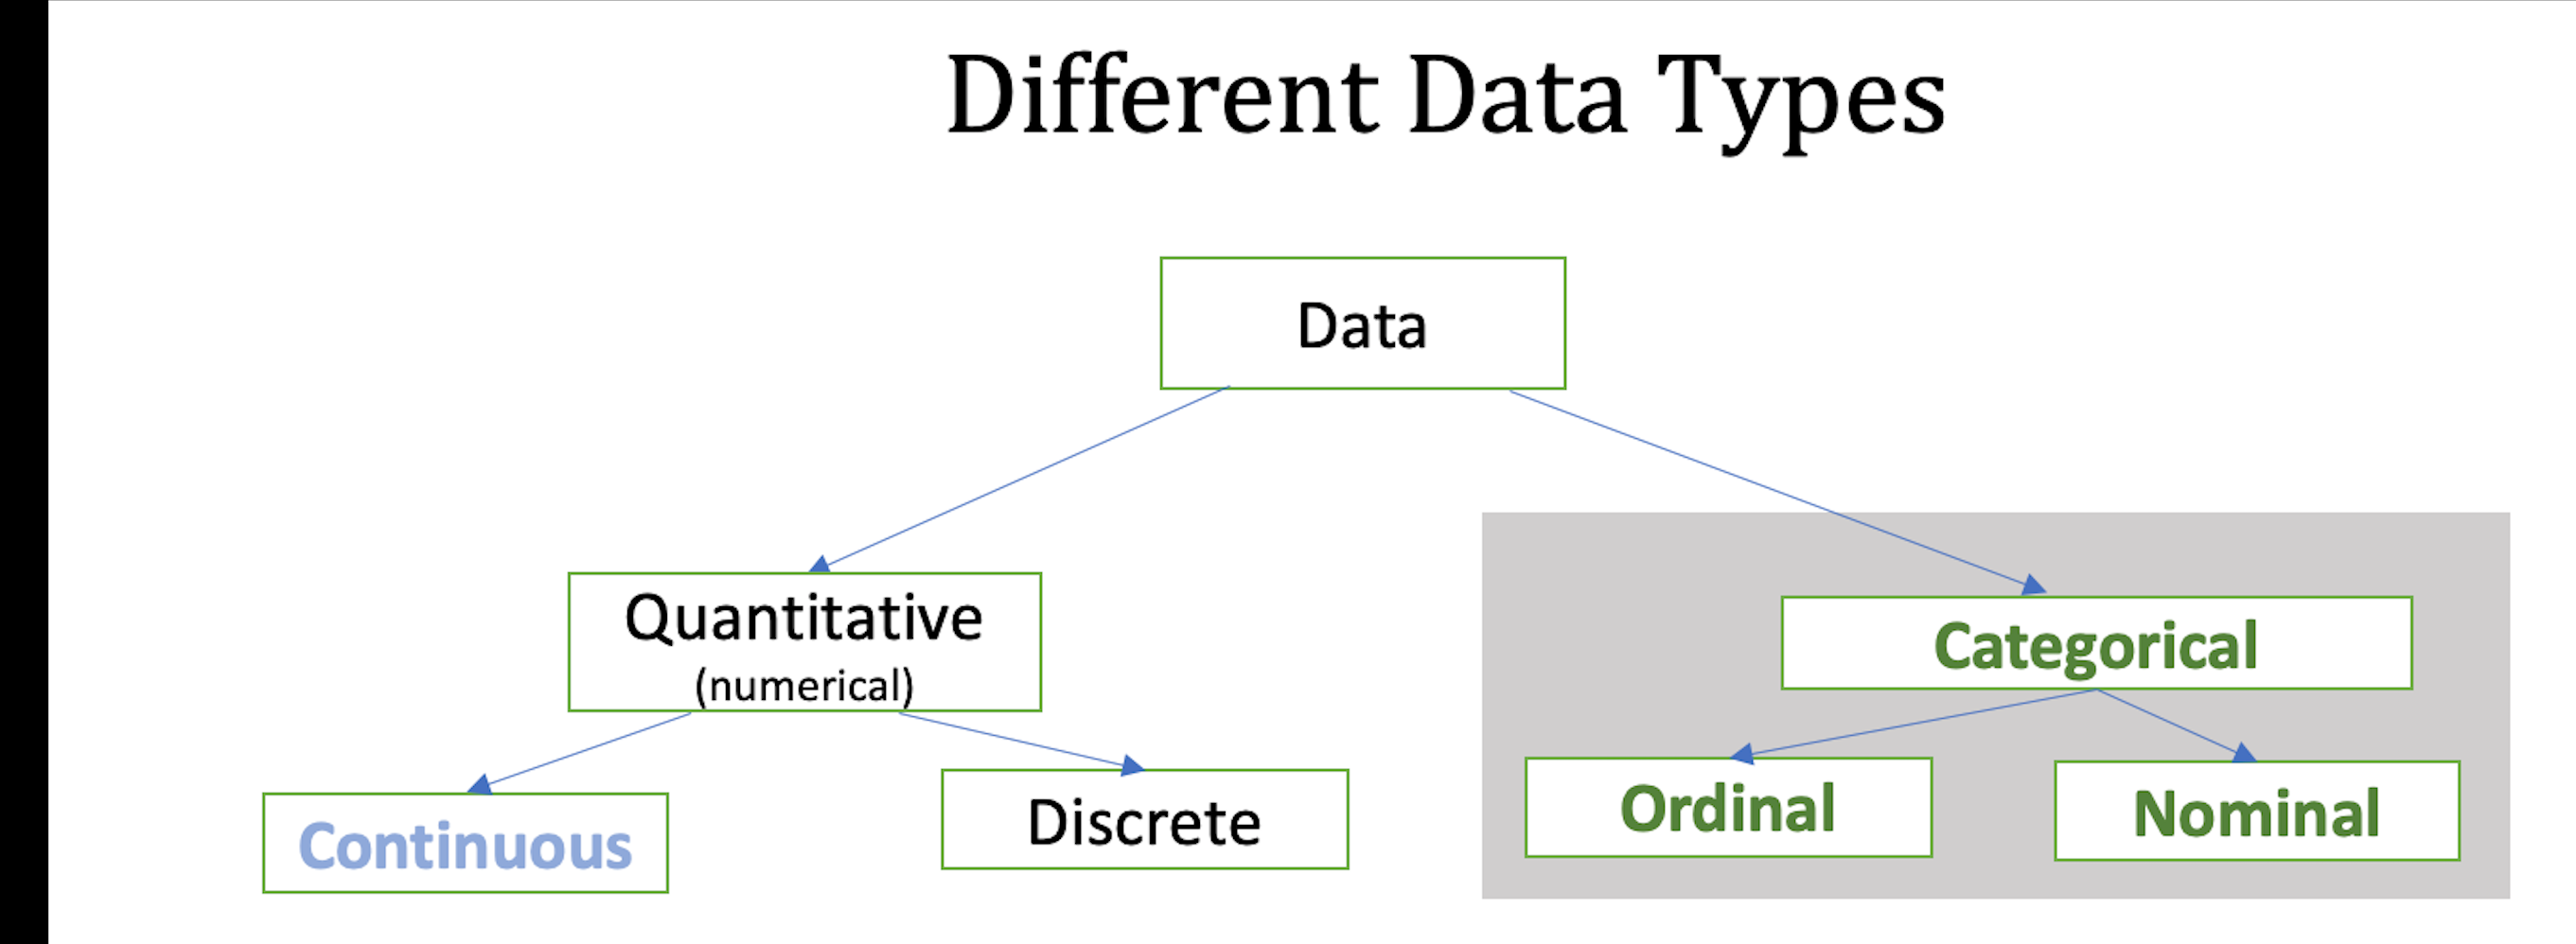
\includegraphics[scale=.25]{typesOFdata1.png} 
\end{frame}



\begin{frame}{ Bernouli Distribution: A probability distribution for the Binary random Variables}

 \qbx[4.1in]{olive!40}{$Y \sim \text{Bernouli}(\pi) $} 
 
 
Support of the random variable:  $Y\in \{0,1\}$\\
Probabilities: $P(Y=1)=\pi$ and $P(Y=0)=1-\pi$

 \qbx[4.1in]{blue!30}{ $E(Y)= \pi$ and $Var(Y)= \pi(1-\pi)$ }. 
\vspace{.1in }
\pause
 \qbx[4.2in]{blue!30}{ Terminology:
 Often, in terms of notation we say:\\
 \qBrd[3.7in]{olive!30}{ $``Y=1" \equiv ``Success"/``Survived" /``Accepted"/``Win"$}  \qBrd[4.1in]{orange!30}{ $``Y=0" \equiv ``Failure"/``Not Survived"/``Not Accepted"/``Loss" $}
  }. 


\end{frame}


\begin{frame}{ Definition: Odds of ``Success"}
 \qbx[4.5in]{teal!40}{{\bf Odds: } The odds of success are defined as the ratio of the probability of success (say, $\pi$) over the probability of failure $(1-\pi)$. \\
 \begin{center}
    \qBrd[2.9in]{blue!30}{$$\text{Odds(``Success")}= \frac{\pi}{1-\pi} $$ }
    \end{center}}\\
    \vspace{1.2in}


\end{frame}



\begin{frame}{ Example: Odds}
 \qbx[4.7in]{teal!40}{{\bf Example: } In a Game of rolling a fair dice twice. A player wins if both throws result in same number. \\
$$ \HLTY{Prob(Win)=\pi=\frac{6}{36}=\frac{1}{6}}, \hspace{1in}\HLTW{Prob(Loss)= 1-\pi =1-\frac{1}{6}=\frac{5}{6}}$$}

\pause

 \begin{center}
    \qBrd[3.5in]{blue!30}{$$\text{Odds(``Win")}= \frac{Prob(Win)}{Prob(Loss)}= \frac{\pi}{1-\pi} = \frac{\frac{1}{6}}{\frac{5}{6}}=\frac{1}{5}$$ }
    \end{center}
\end{frame}








\begin{frame}{ Example: Odds}
 \qbx[4.65in]{teal!40}{{\bf Example: } Probability of 15 years ``survival" of a patient after a critical medical procedure is ``0.9'' \\
$$ \HLTY{Prob(Survival)=\pi=0.9}, \hspace{1in}\HLTW{ 1-\pi =1-0.9=0.1}$$}

\pause

 \begin{center}
    \qBrd[3.5in]{blue!30}{$$\text{Odds(``Survival")}= \frac{Prob(Win)}{Prob(Loss)}= \frac{\pi}{1-\pi} =\frac{0.9}{0.1}= 9$$ }
\qBrd[3in]{teal!40}{Odds of 15 year survival of the patient after the medical procedure is \HLTY{ 9 \text{ to }  1}}
    \end{center}    
    
\end{frame}



\begin{frame}{ Question: Odds}
 \qbx[4.6in]{teal!40}{{\bf Question: } In a game of tossing a fair coin Three times.  A player wins if more number of Heads than that of the Tail.  What is the odds of winning the game? \\
}


\vspace{-.3in}
 \begin{center}
    \qBrd[4.5in]{blue!30}{Probability of Win: \vspace{.5in}}
    \qBrd[4.5in]{blue!30}{ Odds of Win: \vspace{1in}}
    \end{center}
\end{frame}



\begin{frame}{Definition: Logit Function}
 \qbx[4.6in]{teal!40}{{\bf Logit: }Logit  is the natural log of an odds; That is, the logit of a number  $\pi$ between 0 and 1 is given by the formula:\\
 \vspace{-.2in}
 \begin{center}
 \qBrd[3in]{blue!40}{$ \HLTW{\text{Logit}(\pi)}=\log\left(\text{Odds}(\pi)\right)=\HLTW{ \log\left( \frac{\pi}{1-\pi}\right)}$}
 \end{center}
 \vspace{-.1in}
 {\small The range of Logit($\pi$) is $-\infty$ to $\infty$ when the range of $\pi$ is between 0 and 1.
 }
 }
 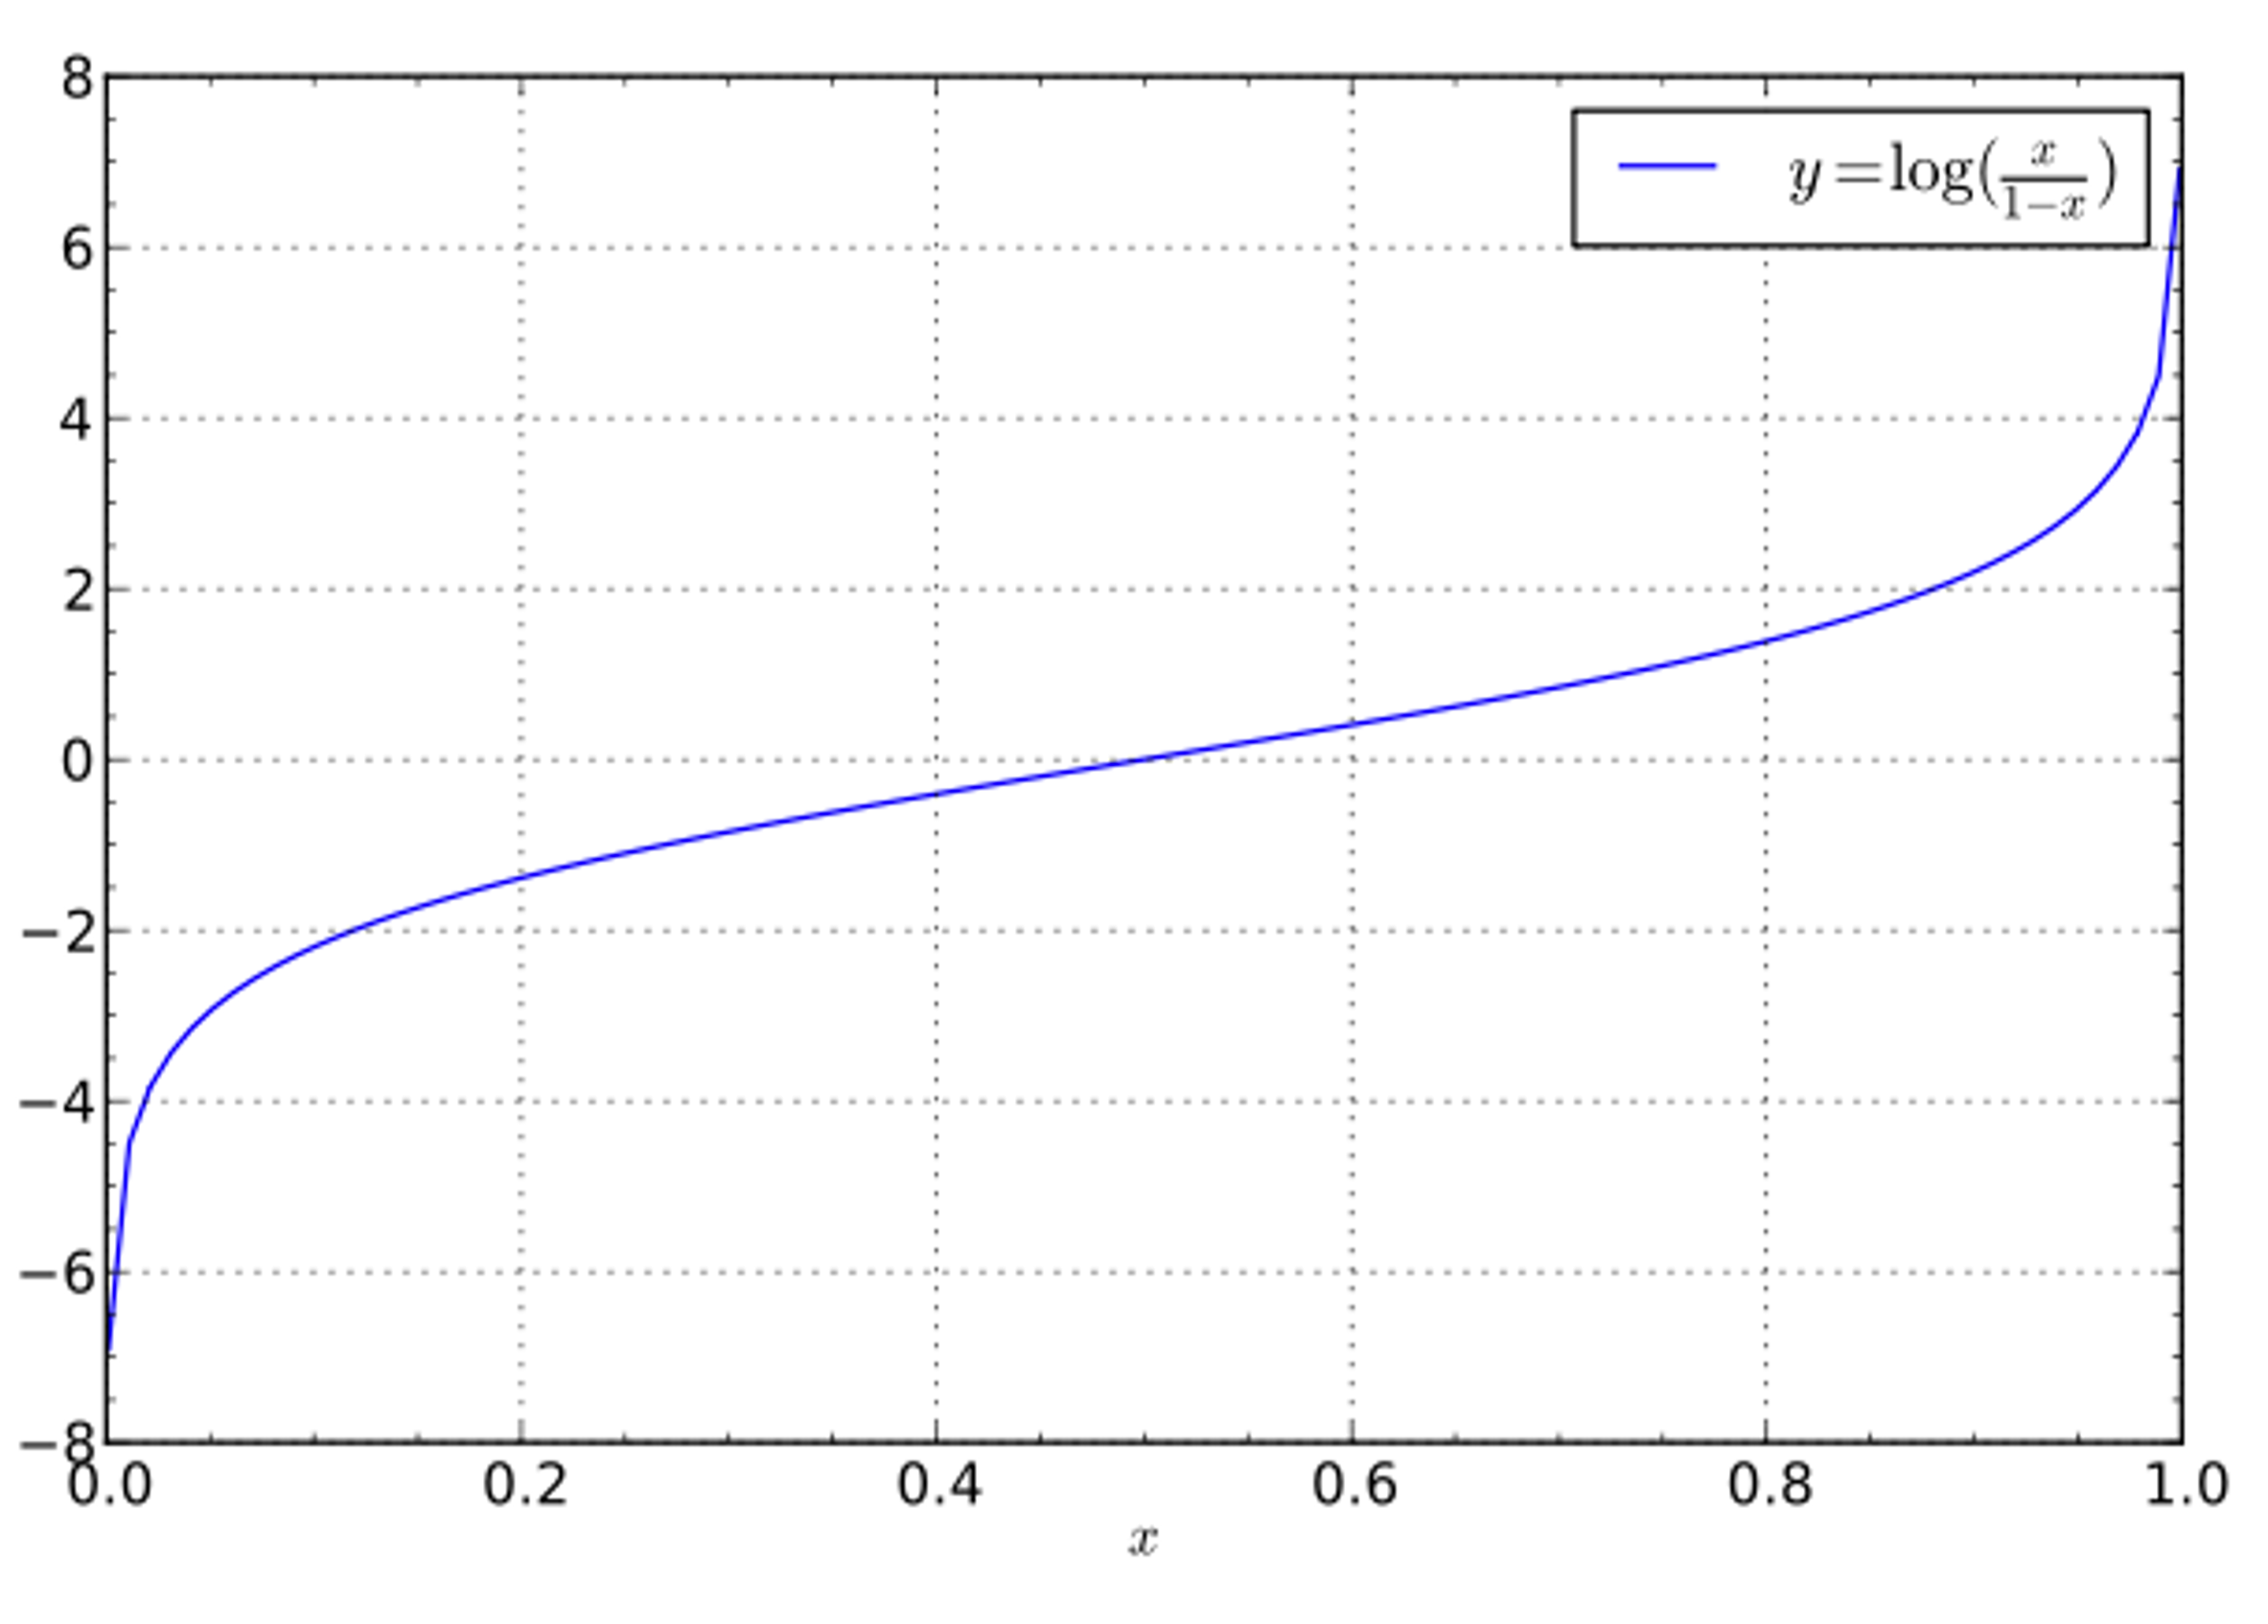
\includegraphics[scale=.16]{Logit_plot.png} 

\end{frame}





\begin{frame}{Definition: Expit Function}
 \qbx[4.6in]{orange!40}{{\bf Expit: }Expit of a number  $x$ between $-\infty$ and $\infty$ is given by:
 \qBrd[1.5in]{olive!40}{$ \HLTW{\text{Expit}(x)}=\HLTW{\frac{e^x}{1+e^x}}$}\\
 {\small The range of Expit($x$) is $0$ to $1$ when the range of $x$ is between $-\infty$ and $\infty$.
 }
 }
 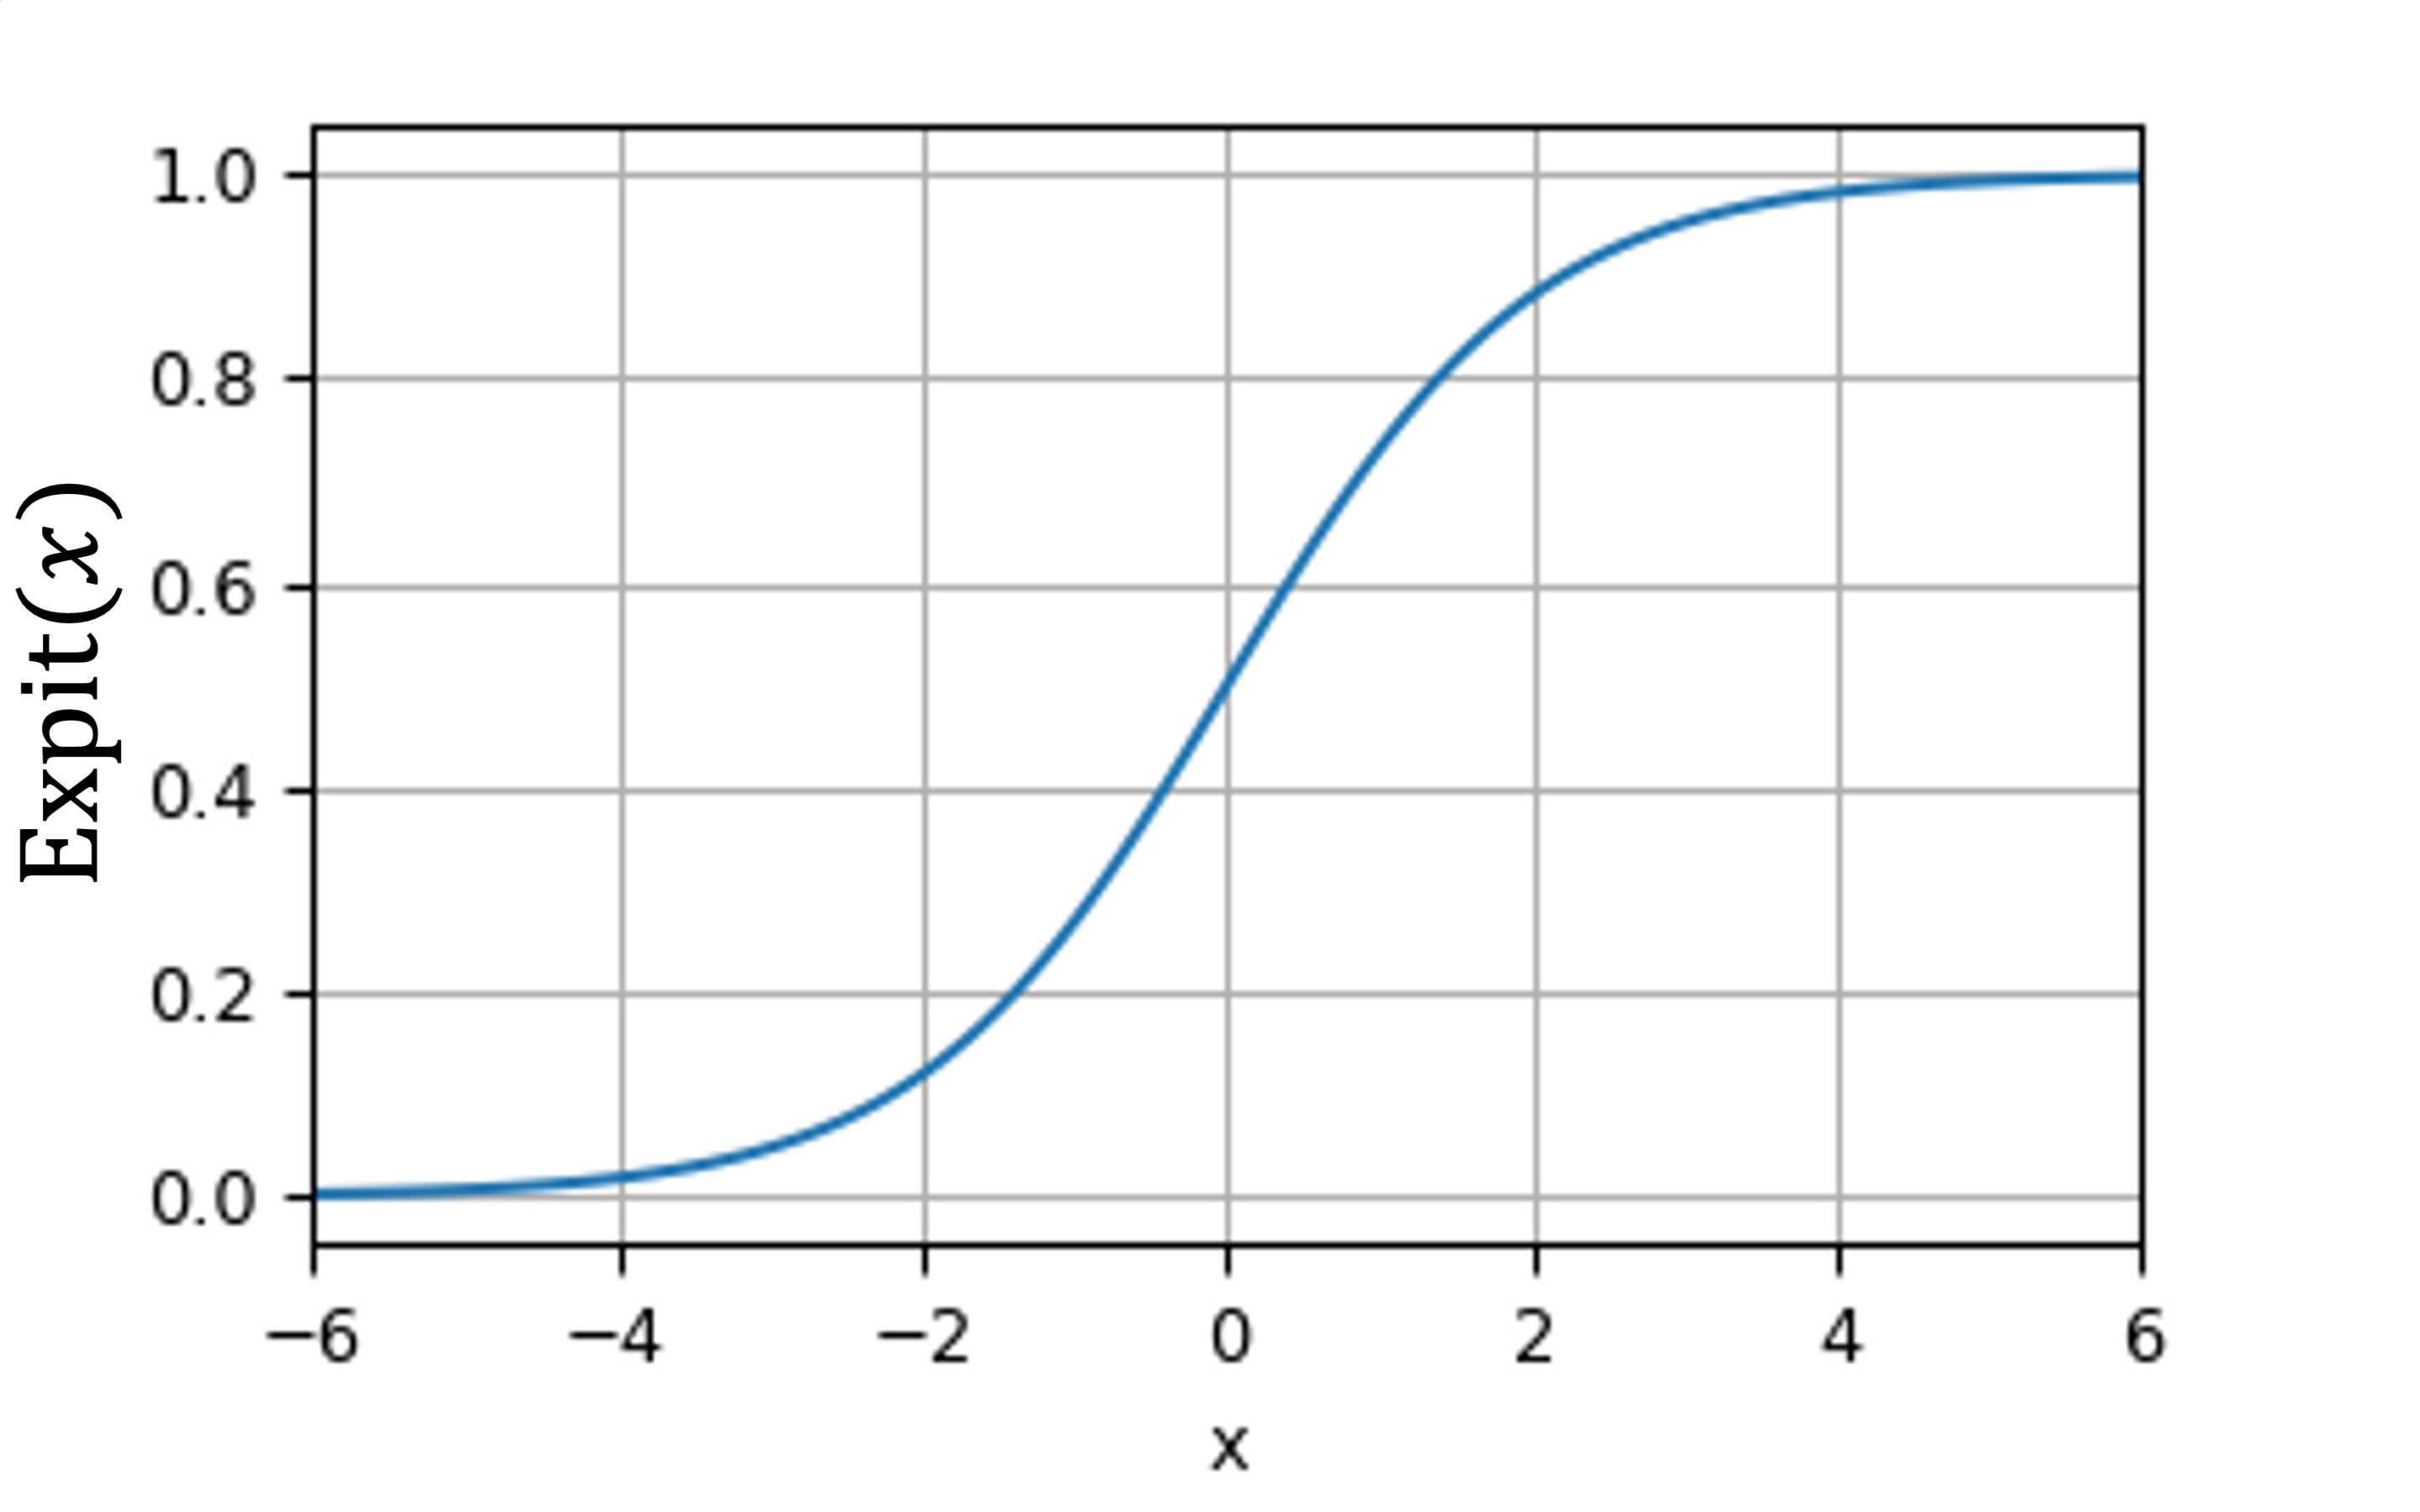
\includegraphics[scale=.15]{Expit_plot.png} 

\end{frame}


\begin{frame}
\qBrd[4.5in]{teal!40}{
$$ \HLTW{\large \frac{e^{V}}{1+e^{V}}}$$
}
\vspace{.02in}
\pause
\qBrd[4.5in]{olive!40}{
$$\Large \HLTW{\large \log(\frac{U}{1-U})}$$
}
\vspace{.02in}
\pause
\qBrd[4.5in]{olive!40}{
$$\Large \HLTW{\large \frac{W}{1-W}}$$
}
\vspace{.02in}
\pause
\qBrd[4.5in]{teal!40}{
$$ \HLTW{\large \frac{e^{\beta_0+\beta_1x}}{1+e^{\beta_0+\beta_1x}}}$$
}
\end{frame}


\begin{frame}
\qBrd[4.5in]{teal!40}{
$\text{Logit}(0.6)=?$
\vspace{.7in}
}
\qBrd[4.5in]{olive!40}{
$\text{Odds}(0.3)=?$
\vspace{.7in}
}

\qBrd[4.5in]{babyblue!40}{
$\text{Expit}(0)=?$
\vspace{.7in}
}
\qBrd[4.5in]{teal!40}{
$\text{Expit}(2)=?$
\vspace{.7in}
}

\end{frame}




\begin{frame}{`Expit' and 'Logit' are Inverse Function to each other}
 \qbx[4.6in]{orange!40}{ \qBrd[2.5in]{olive!40}{$ \text{Expit}(x)= \pi  \implies x= \text{Logit}(\pi)$}\\
  \qBrd[2.5in]{blue!30}{$ \text{Logit}(\pi)= x  \implies \pi= \text{Expit}(x)$}
 }\\
 \pause
 \vspace{1in}
\qbx[4.6in]{orange!40}{ \qBrd[4.5in]{olive!40}{$ \text{Expit}({\color{red} x})= 0.7  \implies x= \text{Logit}(0.7)=\log\left( \frac{0.7}{1-0.7}\right)= \log(\frac{0.7}{0.3}))= \log(2.333)= 0.368$}\\
\vspace{.2in}
  \qBrd[4.5in]{blue!30}{$ \text{Logit}({\color{red}\pi})= 2 \implies \pi= \text{Expit}(2)= \frac{e^2}{1+e^2}=0.88 $}
 }\\
 \vspace{3in}


\end{frame}





\begin{frame}{Question: `Expit' and 'Logit' }
 
 \qBrd[4.5in]{olive!40}{Question: $ \text{Expit}({\color{red} x})= 0.8 \implies x= ?$ \vspace{1.2in}}\\
\vspace{.01in}
  \qBrd[4.5in]{blue!30}{Question: $ \text{Logit}({\color{red}\pi})= -1 \implies \pi= ? $ \vspace{1.2in}}

 \vspace{3in}


\end{frame}





\begin{frame}{Question: 'Logit' and `Odds' }

  \qBrd[4.5in]{teal!30}{Logit and Odds: $ \text{Logit}({\color{red}\pi})= x \implies \HLTY{\text{Odds}(\pi)= \exp(x).} $ \vspace{1.2in}}
 
  \qBrd[4.5in]{blue!30}{Question: $ \text{Logit}({\color{red}\pi})= -1 \implies\text{Odds}(x)=? ? $ \vspace{1.2in}}

 \vspace{3in}


\end{frame}




\begin{frame}{Question: 'Logit' and `Odds' }

  \qBrd[4.5in]{teal!30}{Assume $ \text{Logit}({\color{red}\pi})= \HLTW{\beta_0 + \beta_1 x}$ The compute the following: }
  \qBrd[4.5in]{olive!30}{ $ {\color{red}\pi}= $ \vspace{1in} }
  
 \qBrd[4.5in]{babyblue!30}{ $ \text{Odds}({\color{red}\pi})= $ \vspace{1in} }




\end{frame}




\begin{frame}{`Expit' and 'Logit' are Inverse Function to each other}
\vspace{2in}
 \qbx[4.6in]{lime!40}{ In a logistic regression,  $ \text{Logit}(\pi)$ is modelled instead of a direct modelling of $\pi$.
 }\\
\end{frame}

\TransitionFrame{\Large Logistic Regression}




\begin{frame}{Why There is a Need Logistic Regression ?}
	\vspace{-3mm}
	 \qbx[4.1in]{olive!40}{We have already discussed the \textbf{ linear regression model and their estimation}.\\  \qBrd[3.55in]{blue!10}{ 
	Why do we need additional regression methods?}}
	\vspace{3mm}
	\begin{itemize}
		\item In standard linear regression we assume that the  {\bf Response variable is continuous. }
		\vspace{3mm}
		\item What if the Response variable is {\bf categorical?} in nature?
		%\vspace{3mm}
%		\item[$\rightarrow$] \textbf{target}: Model a dependent \textbf{binary variable} to make an appropriate prediction of probability (using covariates).
\end{itemize}
\end{frame}		


\begin{frame}{Examples of Binary Variables}
	\vspace{-7mm}
Let's imagine independent observations $y_1,\ldots,y_n$ of a
	variable of interest $Y$, which can take \textbf{only two values} (e.g. 0 and 1), e.g.:
	\vspace{3mm}
	\begin{itemize}
		\item Workpiece is defective(1)/not defective(0)
		\vspace{3mm}
		\item Banking: A customer is considered creditworthy: yes(1)/no(0)
		\vspace{3mm}
		\item Health Science: Therapy is successful: yes(1)/no(0).
	\end{itemize}
	
\end{frame}


\begin{frame}
 \qbx[4.1in]{olive!40}{\sqBullet{olive}: Is the standard linear regression \textbf{appropriate} for modeling binary response/dependent variables?}
 \vspace{2.5in}
\end{frame}






\begin{frame}{Reminder: The SLR and Response Type}
\qbx[4.55in]{orange!40}{ \sqBullet{orange} 
The  random sample of size $n$ is denoted as  $\{\HLTY{\by_i} , bx_i\}_{i=1}^n $ where the respone  $\HLTY{\by_i}\in\HLTY{\R}$.}
 \vspace{-.1in}
\qbx[4.55in]{teal!40}{ \sqBullet{teal} The simple linear regression line is given by \vspace{-.1in}
\begin{center}
 \qBrd[1.55in]{blue!10}{ $Y= \alpha+\beta X+\varepsilon.$}  \qBrd[1in]{olive!20}{ $\varepsilon\sim \text{N}(0,\sigma^2)$}\\
 \end{center} }
 \vspace{-.1in}
%}
\pause 

\qbx[4.55in]{orange!40}{ \sqBullet{orange} 
The simple linear regression is not applicable when $\by_i $ NOT continuous. 
}
\qbx[4.55in]{lime!40}{ \sqBullet{lime} 
Specifically,  we use  the logistic regression when the data is  of following type:  random sample of size $n$ is denoted as  $\{\HLTY{\by_i} , \bx_i\}_{i=1}^n $ where  $\HLTY{\by_i}\in \HLTW{\bf  \{0,1\}}$ are responses  and $\bx_i $ pertains to numerical or continuous  covariates.}
\end{frame}

\begin{frame}
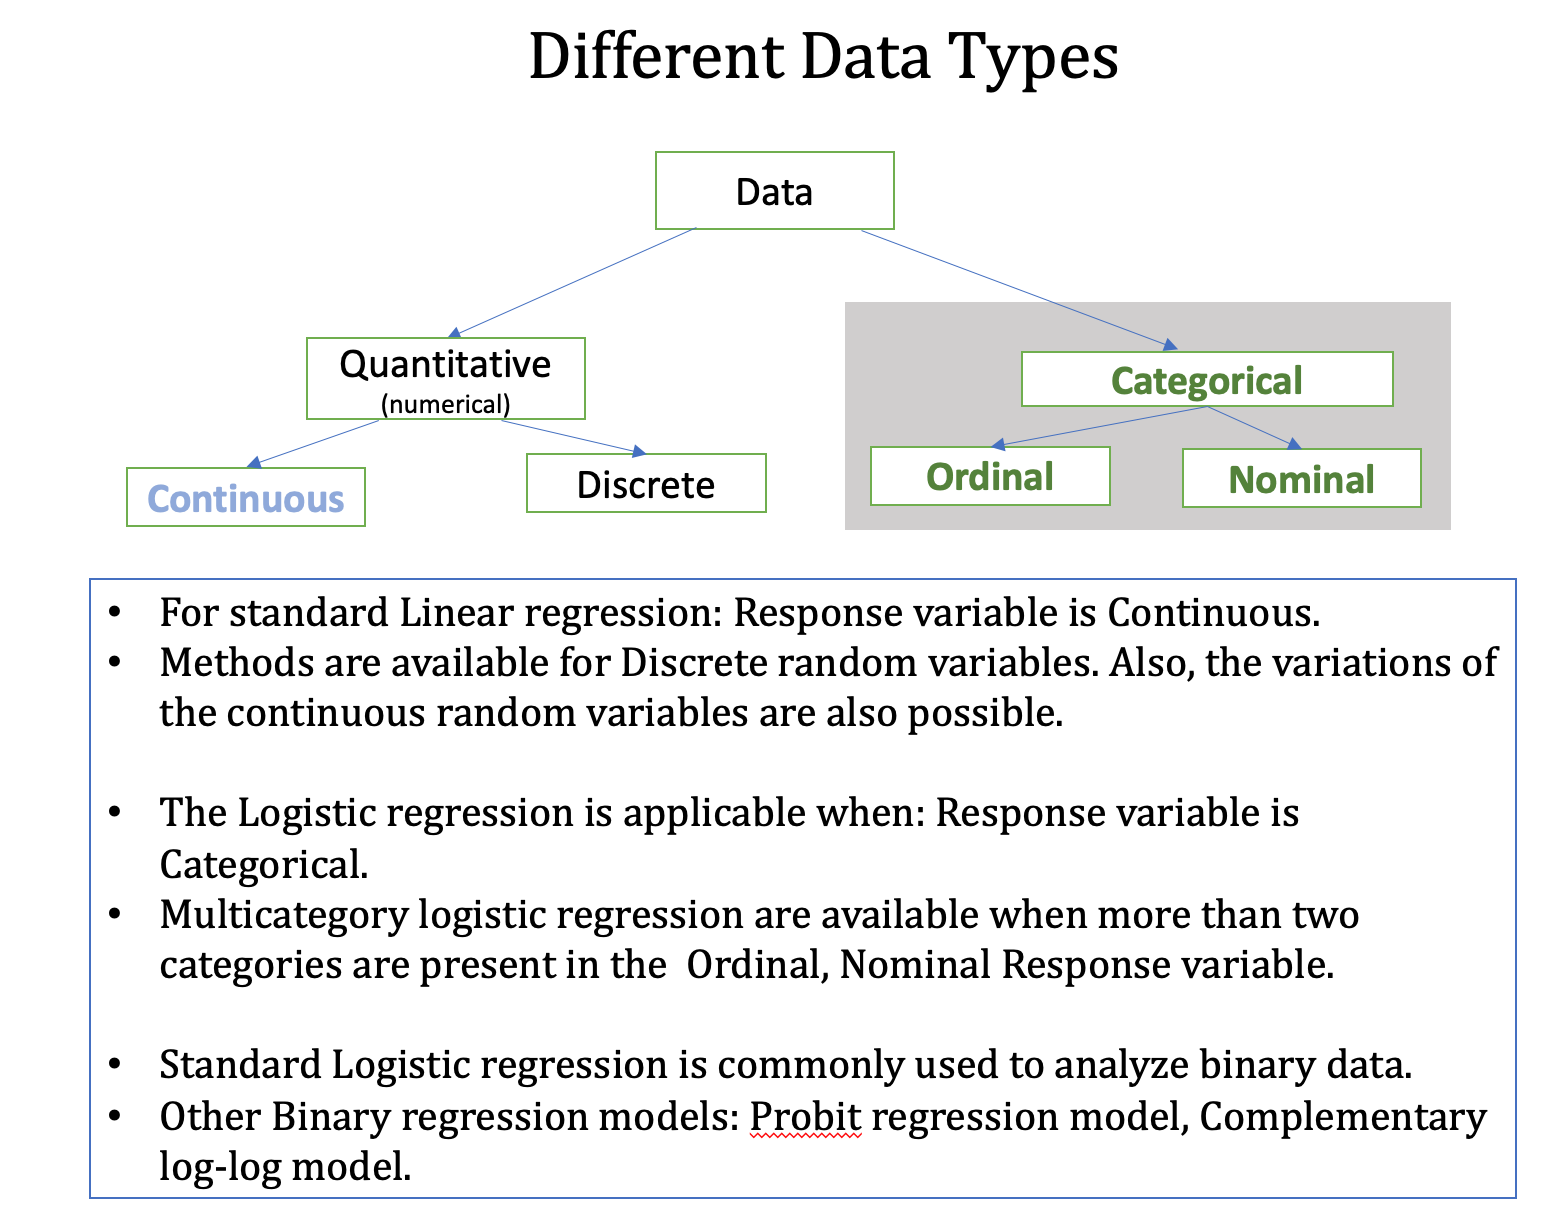
\includegraphics[scale=.4]{typesOFdata.png} 
\end{frame}

\begin{frame}{ Reminder: Bernouli Distribution to model the Response}

 \qbx[4.1in]{olive!40}{$Y \sim \text{Bernouli}(\pi) $} 
 
 
Support of the random variable:  $Y\in \{0,1\}$\\
Probabilities: $P(Y=1)=\pi$ and $P(Y=0)=1-\pi$

 \qbx[4.1in]{blue!30}{In-stead of modeling $Y$ directly we model the probabilities $\pi$}. 
 \qbx[4.6in]{lime!40}{ In particular: In a logistic regression,  $ \text{Logit}(\pi)$ is assumed to be a  function of the covariates. 
 }\\

\end{frame}


\newcommand{\Logit}[1]{\text{Logit}\left( #1\right)}
\newcommand{\Expit}[1]{\text{Expit}\left( #1\right)}
\newcommand{\ExpitExpr}[1]{\frac{e^{#1}}{1+e^{#1}}}
\newcommand{\LogitExpr}[1]{{ \log\left( \frac{#1}{1-\left(#1\right)}\right) }}

\begin{frame}{ The Logistic Regression}
\qbx[4.55in]{teal!40}{ \sqBullet{teal} 
The  random sample of size $n$ is denoted as  $\{\HLTY{\by_i} , bx_i\}_{i=1}^n $ where  $\HLTY{\by_i}\in \{0,1\}$ and $\bx_i $ can be of any type numerical or categorical.}
 \qbx[4.1in]{olive!40}{$\by_i \sim \text{Bernouli}(\pi_i),  0<\pi_i<1. $} 
 
 
 \qBrd[1.5in]{gray!40}{ 
$\pi_i = Prob(Y_i =1)$   
 }\\
 \vspace{.5in}
\qbx[4.6in]{lime!40}{ 
{\bf Model: } \DBX{\Logit{\pi_i}= \bx_i^T \bbeta   }  
 }\\
\vspace{1in}


\end{frame}


\TransitionFrame[violet]{A Few  Results \& Terminology in Logistic Regression }


\TransitionFrame{`Logit Link' and Probability of ``Success'' Logistic Regression}

\begin{frame}{  `Logit' and 'Expit'}
\qbx[4.2in]{lime!40}{ 
 $\Logit{\pi_i}= \bx_i^T \bbeta     
 $}
 \vspace{2in}
 \pause 
\qbx[4.2in]{teal!40}{ 
$\implies\HLTY{ {\pi_i}= \Expit{\bx_i^T \bbeta}  }$   
 }
\end{frame}





\begin{frame}{ Explanation of `Logit' Link}
\qBrd[3 in]{yellow!40}{$$\Huge  {\Huge \boldsymbol{\pi_i}}= {\small \Expit{\bx_i^T \bbeta}  }= \frac{\text{exp}\left( {\bx_i^T \bbeta}\right)}{1+\text{exp}\left( {\bx_i^T \bbeta}\right) }$$}
\vspace{2in}
\end{frame}



\TransitionFrame{`Logit' and 'Odds' in Logistic Regression}

\begin{frame}{ Reminder: Odds of ``Success"}
 \qbx[4.5in]{gray!40}{{\bf Odds: } The odds of success are defined as the ratio of the probability of success (say, $\pi$) over the probability of failure $(1-\pi)$. \\
 \begin{center}
    \qBrd[2.9in]{white!30}{$$\text{Odds(``Success")}= \frac{\pi}{1-\pi} $$ }
    \end{center}}\\
    \vspace{1.2in}


\end{frame}



\begin{frame}{  `Logit' and 'Oddds'}
\qbx[4.6in]{teal!40}{ 
 $\HLTW{\Logit{\pi_i}= \bx_i^T \bbeta}   \implies\HLTY{ \LogitExpr{\pi_i}=  \bx_i^T \bbeta }   
 $}
\\
\vspace{1in} 
 \qbx[4.6in]{blue!40}{ 
 $\implies\HLTY{ \log\left(\HLTW{\text{Odds}{(\pi_i)}}\right)=  \bx_i^T \bbeta  }\implies \HLTY{\HLTW{\text{Odds}{(\pi_i)}} =e^{\bx_i^T \bbeta}  }   
 $}\\
 \vspace{1.4in}
 \DBX{\large $$\HLTW{\Logit{\pi_i}= \bx_i^T \bbeta}   \implies\HLTY{\HLTW{\text{Odds}{(\pi_i)}} =\exp\left({\bx_i^T \bbeta}\right)}$$   }
\end{frame}



\begin{frame}{ 'Odds'  and the `Logit' Link}
\qBrd[3 in]{olive!30}{$$\Huge\HLTW{\text{Odds}{(\pi_i)}} = \text{exp}\left({\bx_i^T \bbeta}\right)$$}
\vspace{2in}
\end{frame}

\TransitionFrame{ Interpretation of a Regression Coefficient: Intercept}
\begin{frame}{ Interpretation of the Intercept}
Let the fitted model be
\qbx[4.6in]{teal!40}{ 
\qBrd[3in]{olive!10}{ $\Logit{\pi_i}=\HLTY{\beta_0} +\beta_1x_{i, 1}+\ldots + \beta_px_{i, p}$} 
 }\\
 
 \qbx[4.6in]{blue!40}{ 
 $\implies$ \qBrd[4in]{olive!30}{$\HLTW{\text{Odds}{(\pi_i)}} =\exp\left(\HLTY{\beta_0} +\beta_1x_{i, 1}+\ldots + \beta_px_{i, p} \right) $}   
 }\\
 \pause
\vspace{.2in } 
 \qbx[4.6in]{blue!40}{ 
 $\implies$ \qBrd[4in]{olive!30}{$\HLTW{\text{Odds}{(\pi_i)}} =\exp\left(\HLTY{\beta_0} +\beta_1\times 0 +\ldots + \beta_p\times 0 \right) = \exp\left(\HLTY{\beta_0} \right)$}, 
 when $x_{i,1}=0, x_{i,2}= 0 , \ldots , x_{i,p}=0.$
 }\\
 \pause
  \qbx[4in]{brown!40}{ 
$ \HLTY{ e^{\beta_0}}$ : Odds that the corresponding Response is 1 when all the covariate values are zero. }
 
\end{frame}


\TransitionFrame{ Interpretation of a Regression Coef.: A Numerical Covariate}

\begin{frame}{ Interpretation of a regression coefficient: numerical variable}
\vspace{-.05in}
\qbx[4.6in]{teal!40}{ 
\qBrd[3in]{olive!10}{ $\Logit{\pi_i}={\beta_0} +\HLTY{\beta_1}\HLTW{x_{i, 1}}+\ldots + \beta_px_{i, p}$} 
Assuming:$ \HLTW{x_{i, 1}}$ to be a numerical covariate.
 }\\
 
 \qbx[4.6in]{blue!40}{ 
 \qBrd[4.5in]{olive!30}{$\HLTW{\text{Odds}{(\pi_i)}\mid_{X_{i,1}=\HLTW{x}}} =\exp\left({\beta_0} +\HLTY{\beta_1}\HLTW{x}+{\beta_2}x_{i, 2}\ldots + \beta_px_{i, p} \right) $}  
  \qBrd[4.6in]{olive!30}{$\HLTW{\text{Odds}{(\pi_i)}\mid_{X_{i,1}=\HLTW{x+1}}} =\exp\left({\beta_0} +\HLTY{\beta_1}(\HLTW{x+1}) +{\beta_2}x_{i, 2}\ldots + \beta_px_{i, p} \right) $}   
 \vspace{-.2in}}\\
 \pause
\vspace{.01in } 
 \qbx[4.6in]{blue!40}{ 
$$ \frac{\HLTW{\text{Odds}{(\pi_i)}\mid_{X_{i,1}=\HLTW{x+1}}} }{ \HLTW{\text{Odds}{(\pi_i)}\mid_{X_{i,1}=\HLTW{x}}}}= \text{exp}(\HLTY{\beta_1}). $$
\vspace{-.13in}
 }\\
 
\end{frame}




\begin{frame}{ Interpretation of a regression coefficient corresponding to a numerical variable}

\vspace{.01in } 
 \qbx[4.6in]{blue!40}{ 
$$ \frac{\HLTW{\text{Odds}{(\pi_i)}\mid_{X_{i,1}=\HLTW{x+1}}} }{ \HLTW{\text{Odds}{(\pi_i)}\mid_{X_{i,1}=\HLTW{x}}}}= \text{exp}(\HLTY{\beta_1}). $$
\vspace{-.1in}
 }\\
 \qbx[4.6in]{teal!40}{ 
$$ {\HLTW{\text{Odds}{(\pi_i)}\mid_{X_{i,1}=\HLTW{x+1}}} }= \text{exp}(\HLTY{\beta_1}){ \HLTW{\text{Odds}{(\pi_i)}\mid_{X_{i,1}=\HLTW{x}}}}. $$
\vspace{-.1in}
 }\\
 \pause
  \qbx[4.6in]{brown!40}{ 
$ \HLTY{ e^{\beta_1}}$ : If all other variables remain fixed,  the Odds of ``Succcess ($Y_i=1$)'' is changed by the factor  $\HLTY{e^{\beta_1}}$ when the $x_{1, i}$ is {\bf increased by} 1.   }
 
\end{frame}




\begin{frame}{ Finally: Interpretation of a regression coefficient corresponding to a numerical variable}

\vspace{.01in } 
 \qbx[4.6in]{blue!40}{ 
$$ \frac{\HLTW{\text{Odds}{(\pi_i)}\mid_{X_{i,1}=\HLTW{x+1}}} }{ \HLTW{\text{Odds}{(\pi_i)}\mid_{X_{i,1}=\HLTW{x}}}}= \text{exp}(\HLTY{\beta_1}). $$
\vspace{-.1in}
 }\\
 \hspace{-.4in}\qbx[4.8in]{cyan!40}{ 
$$ \frac{\HLTW{\text{Odds}{(\pi_i)}\mid_{X_{i,1}=\HLTW{x+1}}}   -  \HLTW{\text{Odds}{(\pi_i)}\mid_{X_{i,1}=\HLTW{x}}}}{ \HLTW{\text{Odds}{(\pi_i)}\mid_{X_{i,1}=\HLTW{x}}}}\times 100\%=\left( \HLTY{e^{\beta_1}}-1\right)\times 100\%. $$
\vspace{-.1in}
 }\\
 \pause
  \qbx[4.6in]{lime!40}{ 
$ \HLTY{ (e^{\beta_1}-1)\times 100\%}$ : If all other variables remain fixed,  the Odds of ``Success ($Y_i=1$)'' is increased ({\small decreased  if it is a negative number}) by   $(\HLTY{e^{\beta_1}}-1)\times 100\%$ when the variable $x_{1, i}$ is {\bf increased by} 1.   }
 
\end{frame}





\TransitionFrame{ Interpretation of Regression Coefficient: A Categorical Covariate}



\begin{frame}{ Interpretation of a reg. coeff. : Categorical Covariate}
\vspace{-.05in}
\qbx[4.6in]{teal!40}{ 
\qBrd[3in]{olive!10}{ $\Logit{\pi_i}={\beta_0}+   \beta_1x_{i, 1}+\HLTY{\beta_2}\HLTW{x_{i, 2}}+\ldots + \beta_px_{i, p}$} 
Assume:$ \HLTW{x_{i, 2}}$ to be a Categorical Gender variable.  $x_{i, 2}=1$ for Female and $x_{i, 2}=0$ for Male.
 }\\
 
 \qbx[4.6in]{blue!40}{ 
 \qBrd[4.5in]{olive!30}{$\HLTW{\text{Odds}{(\pi_i)}\mid_{_{'Male'}}} =\exp\left({\beta_0} +\beta_1x_{i, 1}+\HLTY{\beta_2}\HLTW{0}+{\beta_2}x_{i, 2}\ldots + \beta_px_{i, p} \right) $}  
  \qBrd[4.6in]{olive!50}{$\HLTEQ[pink!70]{\text{Odds}{(\pi_i)}\mid_{_{'Female'}}} =\exp\left({\beta_0} +\beta_1x_{i, 1}+\HLTY{\beta_2}(\HLTW{1}) +{\beta_2}x_{i, 2}\ldots + \beta_px_{i, p} \right) $}   
 \vspace{-.2in}}\\
 \pause
\vspace{.01in } 
 \qbx[3.6in]{blue!40}{ 
$$ \frac{\HLTEQ[pink]{\text{Odds}{(\pi_i)}\mid_{_{`Female'}}} }{ \HLTW{\text{Odds}{(\pi_i)}\mid_{_{`Male'}}}}= \text{exp}(\HLTY{\beta_2}). $$
\vspace{-.13in}
 }\\
\end{frame}




\begin{frame}{ Interpretation:  Regression Coefficient for a Categorical Covariate}

\vspace{.01in } 
 \qbx[4.6in]{blue!40}{ 
$$ \frac{\HLTEQ[pink!60]{\text{Odds}{(\pi_i)}\mid_{_{`Female'}}} }{ \HLTW{\text{Odds}{(\pi_i)}\mid_{_{`Male'}}}}= \text{exp}(\HLTY{\beta_2}). $$
\vspace{-.1in}
 }\\
  \vspace{.1in}
 \qbx[4.6in]{teal!40}{ 
$$ {\HLTEQ[pink!60]{\text{Odds}{(\pi_i)}\mid_{_{`Female'}}} }= \text{exp}(\HLTY{\beta_2}){ \HLTW{\text{Odds}{(\pi_i)}\mid_{_{`Male'}}}}. $$
\vspace{-.1in}
 }\\
 \pause
 \vspace{.1in}
  \qbx[4.6in]{babyblue!50}{ 
$ \HLTY{ e^{\beta_2}}$ : Assuming all other variables remain fixed,  the Odds of  ``Succcess ($Y_i=1$)'' for a datapoint corresponding to the category $\HLTEQ[pink!60]{`Female'}$ is  $\HLTY{e^{\beta_2}}$  times the Odds of a data point with the category  $ \HLTW{`Male'}$      }
 
\end{frame}



\begin{frame}{Finally:  Interpretation:  Regression Coefficient for a Categorical Covariate}

\vspace{.01in } 
\qbx[4.6in]{blue!40}{ 
$$ \frac{\HLTEQ[pink!60]{\text{Odds}{(\pi_i)}\mid_{_{`Female'}}} }{ \HLTW{\text{Odds}{(\pi_i)}\mid_{_{`Male'}}}}= \text{exp}(\HLTY{\beta_2}). $$
\vspace{-.1in}
 }\\
 \hspace{-.4in}\qbx[4.8in]{cyan!40}{ $$ \frac{\HLTEQ[pink!60]{\text{Odds}{(\pi_i)}\mid_{_{`Female'}}} -  \HLTW{\text{Odds}{(\pi_i)}\mid_{_{`Male'}}}}{ \HLTW{\text{Odds}{(\pi_i)}\mid_{_{`Male'}}}}
\times 100\%=\left( \HLTY{e^{\beta_1}}-1\right)\times 100\%. $$
\vspace{-.1in}
 }\\
 \pause
  \qbx[4.6in]{lime!40}{ 
$ \HLTY{ (e^{\beta_1}-1)\times 100\%}$ : If all other variables remain fixed,  the Odds/Chance of ``Success ($Y_i=1$)'' for a ${\HLTEQ[pink!60]{`Female'}} $ is  $(\HLTY{e^{\beta_1}}-1)\times 100\%$  {\bf more}  ({\small {\bf less}  if it is a negative number}) compared to the corresponding Odds/Chance for a {$\HLTW{`Male'}$}.    }
 
\end{frame}





\begin{frame}

\end{frame}
%
%
\begin{frame}{Interpretation of coefficients: Summary}
	\vspace{-3mm}
\begin{itemize}
	\item
	The direct interpretation of the $\hat{\beta}$ is highly nontrivial and often non-intuitive. 
 	\item 
	Therefore, in Logistic regression, it is common practice  to interpret the  $\HLTY{\exp(\hat{{\beta}})}$ which has a straightforward interpretation with Odds. 
\end{itemize}
\begin{table}[ht]
	\centering
	\begin{tabular}{cccc}
	\hline
 $\hat{{\beta}}$ &  $\text{Odds}(\pi_i)=\frac{P(Y_i = 1)}{P(Y_i = 0)}$ & $\% $change in Odds &  $P(Y_i = 1)$\\ 
	\hline
$\hat{{\beta}}> 0$ & increases by $\HLTY{\exp(\hat{{\beta}})}$ &  $\HLTY{\tiny (\exp(\hat{{\beta}})-1)\times 100\%}$  & increases \\& & &  \\
$\hat{{\beta}}< 0$ & decreases by $\HLTY{\exp(\hat{{\beta}})}$& $\HLTY{\tiny (\exp(\hat{{\beta}})-1)\times 100\%}$  &  decreases\\& & &  \\
$\hat{{\beta}} = 0$ &remains the  same &  $0\%$ &  same \\
	\hline
	\end{tabular}
\end{table}
\end{frame}


\TransitionFrame{A Data Example}









\begin{frame}{Awards Data}

  \qBrd[4.6in]{blue!40}{ 
  The Dataset have two columns.   'Award' and 'Read'
  }

  \qBrd[4.6in]{olive!40}{ 
  \sqBullet{olive} \HLTW{'Award'}: Indicates whether a student obtained the Award or not.  
  }

  \qBrd[4.6in]{teal!40}{ 
  \sqBullet{teal}\HLTW{'Read'}:  Hours the student have spend in additional literature study. 
  }\\
  \vspace{.1in}
  
    \qbx[4.6in]{pink!70}{ 
  \sqBullet{pink} We want to model the response `Award' based on the numerical covariate 'Read'.
  }
  

\end{frame}


\begin{frame}
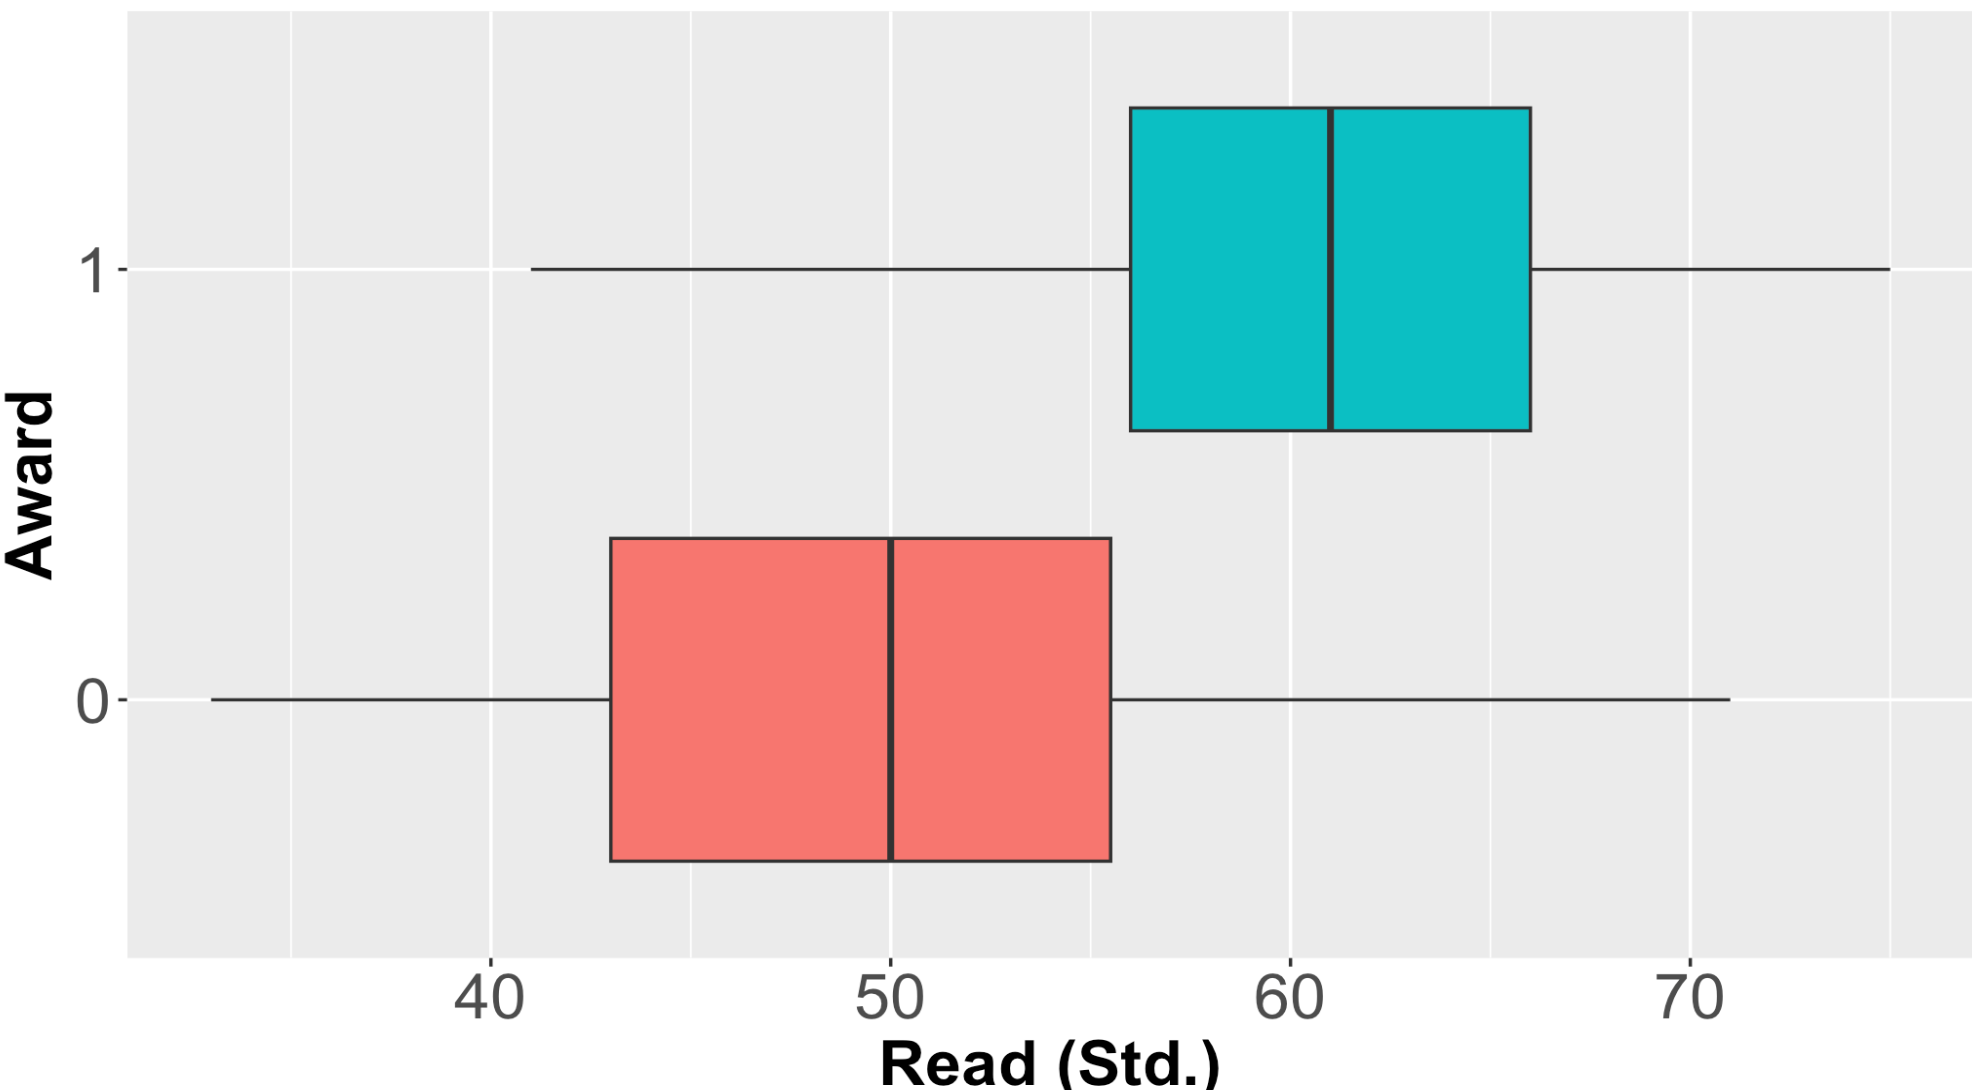
\includegraphics[scale=.3]{BOXPLOT_AWARD.png} 
\end{frame}







\begin{frame}

  \qBrd[4.6in]{gray!95}{ \color{white}
  $model.lr\text{<-} glm(Award \sim  Read, data = performance,  family = "binomial")$\\
  \\
$summary(model.lr)$
}

\end{frame}



\begin{frame}
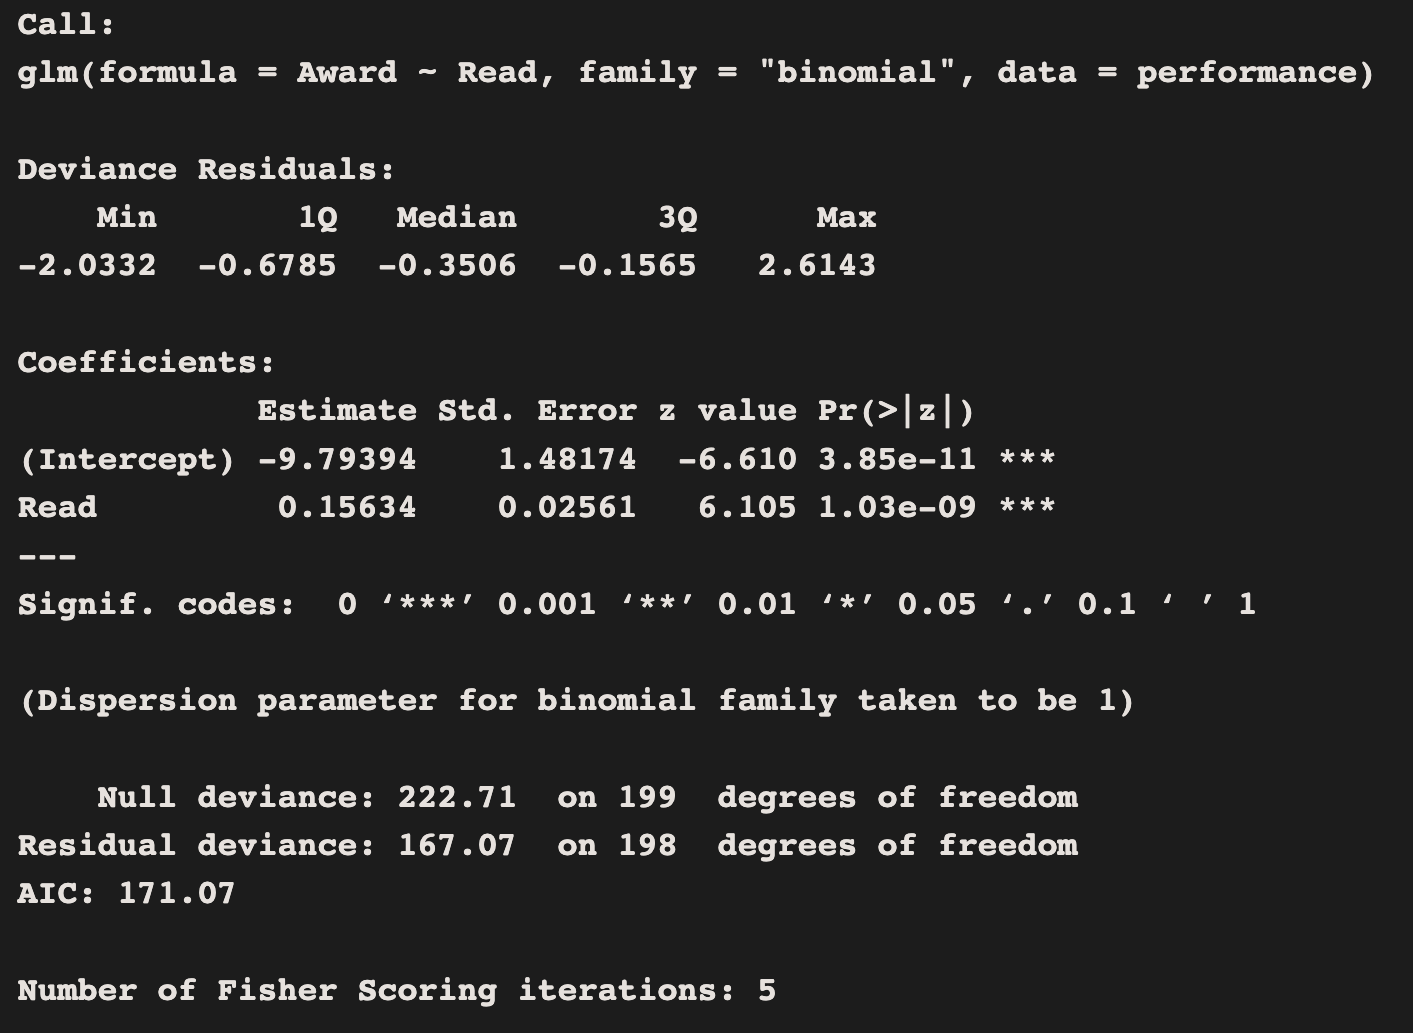
\includegraphics[scale=.45]{LROut.png} 
\end{frame}


\begin{frame}{Reminder: Interpretation of coefficients}
	\vspace{-3mm}
\begin{itemize}
	\item
	The direct interpretation of the $\hat{\beta}$ is highly nontrivial and often non-intuitive. 
 	\item 
	Therefore, in Logistic regression, it is common practice  to interpret the  $\HLTY{\exp(\hat{{\beta}})}$ which has a straightforward interpretation with Odds. 
\end{itemize}
\begin{table}[ht]
	\centering
	\begin{tabular}{cccc}
	\hline
 $\hat{{\beta}}$ &  $\text{Odds}(\pi_i)=\frac{P(Y_i = 1)}{P(Y_i = 0)}$ & $\% $change in Odds &  $P(Y_i = 1)$\\ 
	\hline
$\hat{{\beta}}> 0$ & increases by $\HLTY{\exp(\hat{{\beta}})}$ &  $\HLTY{\tiny (\exp(\hat{{\beta}})-1)\times 100\%}$  & increases \\& & &  \\
$\hat{{\beta}}< 0$ & decreases by $\HLTY{\exp(\hat{{\beta}})}$& $\HLTY{\tiny (\exp(\hat{{\beta}})-1)\times 100\%}$  &  decreases\\& & &  \\
$\hat{{\beta}} = 0$ &remains the  same &  $0\%$ &  same \\
	\hline
	\end{tabular}
\end{table}
\end{frame}


\begin{frame}{Illustration: interpretation of results}
	\vspace{-3mm}
\begin{itemize}
		\item 
	Model to be estimated: $P(AWARD=1\mid READ)=\frac{\exp{(\beta_0 + \beta_1*Read)}}{1 + \exp{(\beta_0 + \beta_1*Read)}}$
		\vspace{0.2cm}
	\item Estimated parameter:  $\hat{{\beta_1}}=0.15634$ (Regression coefficient corresponding to the variable 'Read')
	\end{itemize}
		
	  \qBrd[4.2in]{teal!35}{  \sqBullet{teal} $\HLTY{e^{\hat{\beta}_1}=\exp(0.15634) = 1.1692}$: For each hour increment in the variable 'Read' ( Study time aiming the award), on average, the Odds/chance for a student to win the prize in increased by a factor of  $\HLTY{1.1692}$ times.}
	\vspace{0.2cm}	
	\pause
 \qBrd[4.2in]{olive!35}{  \sqBullet{olive} $\HLTY{(e^{\hat{\beta}_1-1)}\times 100\%=16.92\%}$: For each hour increment in the variable 'Read' ( Study time aiming the award), on average, a student have $\HLTY{16.92}\%$  more Odds/chance to win the prize.}
	\vspace{0.2cm}	
\end{frame}




\begin{frame}{Illustration: interpretation of results}
	\vspace{-3mm}
\begin{itemize}
		\item 
	Model to be estimated: $P(AWARD=1\mid READ)=\frac{\exp{(\beta_0 + \beta_1*Read)}}{1 + \exp{(\beta_0 + \beta_1*Read)}}$
		\vspace{0.2cm}
	\item Estimated parameter:  $\hat{{\beta_0}}=-9.79394$ (Regression coefficient corresponding to the variable 'Read')
	\end{itemize}
		
	  \qBrd[4.2in]{blue!35}{  \sqBullet{teal} $\HLTY{e^{\hat{\beta}_0}=\exp(-9.79394) < 0.00006}$:  On an average,  the Odds/Chance for a student to win the Award is less than  $\HLTY{0.00006}$ if he/she spends 0 hours of Reading.}
\end{frame}





\begin{frame}{Illustration: interpretation of results}
	\vspace{-3mm}

  \qBrd[4.2in]{teal!35}{  \sqBullet{teal} What is the estimated probability of wining the prize for a student, if she/she spends 70 hours of Read?}
	
	\vspace{0.2cm}	
	  \qBrd[4.2in]{olive!35}{ 
 $\HLTY{\frac{\exp{(-9.8+0.16*70)}}{1 + \exp{(-9.8+0.16*70)}}=0.8}$: The estimated probability of wining the prize for a student, if she/she spends 70 hours of Read is 0.80.
	}

\end{frame}





%
%
%
%%%%%%%%%%%%%%%%%%%%%%%%%%%%%%%%
%
%
%
%
%
%
%\begin{frame}{$R^2$ Goodness of Fit }
%\qbx[4.5in]{blue!40}{ $$\HLTW{ \text{ESS}= \sum_{i=1}^{n}(y_i- \hat{y}_i)^2} \text{ \tiny and } \HLTY{ \text{RMSE}= \sqrt{\frac{\sum_{i=1}^{n}(y_i- \hat{y}_i)^2}{n}}} $$   $$ \HLTW{ \text{TSS}= \sum_{i=1}^{n}(y_i- \bar{Y})^2} $$  $$ \HLTW{ \text{SSR}= \sum_{i=1}^{n}(\hat{y}_i- \bar{Y})^2} $$  }
%\qbx[3in]{olive!40}{ 
%Result: $$ \HLTY{  \text{TSS}= \text{ESS}+  \text{SSR}.} $$
%}
%
%\qbx[3in]{teal!30}{ 
%$$ R^2 = 1- \frac{ESS}{TSS}  =  1- \frac{\sum_{i=1}^{n}(y_i- \hat{y}_i)^2}{\sum_{i=1}^{n}(y_i- \bar{Y})^2}  $$
%}
%
%\end{frame}
%
%
%
%
%
%\begin{frame}{Adjusted-$R^2$ Goodness of Fit }
%\qbx[4.5in]{blue!40}{ $$\HLTW{ \text{ESS}= \sum_{i=1}^{n}(y_i- \hat{y}_i)^2},  $$  $$ \HLTW{ \text{TSS}= \sum_{i=1}^{n}(y_i- \bar{Y})^2} $$  $$ \HLTW{ \text{SSR}= \sum_{i=1}^{n}(\hat{y}_i- \bar{Y})^2} $$  }
%
%\begin{center}
%
%\qbx[3in]{olive!40}{ 
%$$ R_{_{\text{adj}}}^2 = 1- \frac{\frac{ESS}{n-p}}{\frac{TSS}{n-1}}  = \HLTW{\displaystyle 1- \frac{n-1}{n-p} (1-R^2)}.  $$
%}
%\end{center}
%
%here $p=2$ as we have only two regression coefficients, namely  $\alpha, \beta$.
%
%\end{frame}
%
%
%\begin{frame}{F Statistic: Model Fitness}
%\qbx[4.5in]{blue!40}{ $$\HLTW{ \text{ESS}= \sum_{i=1}^{n}(y_i- \hat{y}_i)^2}  $$   $$ \HLTW{ \text{TSS}= \sum_{i=1}^{n}(y_i- \bar{Y})^2} $$  $$ \HLTW{ \text{SSR}= \sum_{i=1}^{n}(\hat{y}_i- \bar{Y})^2} \vspace{-.15in} $$  }
% \begin{center}
%\qbx[3in]{olive!40}{ 
%Result: $$ \HLTY{  \text{TSS}= \text{ESS} + \text{SSR}.} \vspace{-.15in} $$
%}\vspace{.01in}
%
%\qbx[3in]{teal!30}{ 
%$$ F= \frac{\frac{SSR}{p-1}}{\frac{SSE}{n-p}} \sim \text{F}_{_{(p-1), (n-p)} \text{df}} \vspace{-.15in} $$
%}
% 
% \end{center}
%$p$ denotes the total number of regression coefficients including the intercept.  Here $p=2$ as we have only two regression coefficients $\alpha, \beta$.
%
%\end{frame}
%
%
%
%\TransitionFrame{\Large Model Selection Criterion: \\
% AIC, BIC  }
%
%
%
%
%
%
%
%
%
%\definecolor{almond}{rgb}{0.94, 0.87, 0.8}
%\definecolor{asparagus}{rgb}{0.53, 0.66, 0.42}
%
%
%
%
%\begin{frame}{  Likelighood of The Linear Statistical Model}
%\qBrd[1.55in]{almond!70}{ $\MakeVec{y}= X\bbeta+\MakeVec{\varepsilon}.$}  \qBrd[2in]{olive!20}{ $\MakeVec{\varepsilon}\sim \text{N}(0,\sigma^2I_{n\times n})$}
%
%
%
%
%
%\qBrd[4.4in]{almond!70}{ 
%Likelihood of the data:= Probability Density of the Response
%}
%
%\qBrd[4.4in]{olive!30}{ 
%Likelihood:=\DBX{ \frac{1}{\left(\sqrt{2\pi}\sigma\right)^n }e^{-\frac{(\MakeVec{y}-X\bbeta)^T (\MakeVec{y}-X\bbeta)}{2\sigma^2}}
%}}
%\vspace{.01in}
%
%\qBrd[4.4in]{olive!30}{ 
%Log Likelihood:=\DBX{n\log\left(\sqrt{2\pi}\sigma\right)
%{-\frac{(\MakeVec{y}-X\bbeta)^T (\MakeVec{y}-X\bbeta)}{2\sigma^2}}
%}}
%
%
%\qBrd[4.4in]{green!30}{ Maximum Likelihood Principle: 
%{\bf Larger Value for the Likelihood/ Log Likelihood indicates a better model fit.} }
%
%
%
%
%
%
%\end{frame}
%
%
%
%
%
%
%\begin{frame}{  Model selection: Akaike's Information Criteria (AIC)}
%\qBrd[4.6in]{almond!70}{ The AIC Criterion for a General model is:\\ \DBX{AIC =2\HLTY{ p }- 2\times \text{Log-Likelihood}\left(\text{Model}\right).   } Here \HLTY{ p }: denotes the model dimension/ model complexity.
%}
%
%
%\vspace{-.1in}
%\qBrd[4in]{green!40}{ 
%Identify the one among the competing models that have the {\bf smallest AIC.}
%}
%
%\end{frame}
%
%
%
%\begin{frame}{  Model selection: Schwarz's  Bayesian information criterion (BIC) }
%\qBrd[4.6in]{almond!70}{ The BIC Criterion for a General model is:\\ \DBX{BIC =\HLTY{ p }\log(n)- 2\times \text{Log-Likelihood}\left(\text{Model}\right).   } Here \HLTY{ p }: denotes the model dimension/ model complexity.
%}
%
%\vspace{-.1in}
%\qBrd[4in]{green!70}{ 
%Identify the one among the competing models that have the {\bf smallest BIC.}
%}
%
%\end{frame}
%
%
%
%
%\TransitionFrame[slateblue]{\Large Outlier, Influential Points  and Leverages}
%
%
%\begin{frame}{Assumptions of SLR }
%
%\qBoxCol{teal!30}{
%The observed data: $\{Y_i, X_i\}_{i=1}^n $.  According to the model: \HLTY{Y_i= \alpha+\beta X_i+\varepsilon_i}
%}
%
%
%\begin{enumerate}
%\item $\varepsilon_i\sim \text{Normal}(0, \sigma^2)$, $\sigma^2>0$.
%\item $\varepsilon_1, \varepsilon_2, \ldots, \varepsilon_n$ are {\it statistically  independent} (i.e.  random and unrelated. )
%\item $\sigma^2$  ( likely to be unknown ) is constant. It does not depend on the responses of the covariates. 
%\end{enumerate}
%\qBrd{teal!30}{Apart from checking the model assumptions, we also need to be cautious if there is any outlier/influential points in the data. }
%
%\end{frame}
%
%
%
%
%
%\begin{frame}{Assumptions of SLR }
%\qBoxCol{teal!30}{
%Need to check whether the data set does not violate any of the assumptions mentioned in the previous slide.
%}
%
%\qBrd{olive!40}{What else can go wrong?}
%\begin{enumerate}
%\item Regression function can be wrong- missing predictors,
%nonlinearity
%\item Outliers: both in predictors and observations.
%\item Influential Points: these points have high  influence on the
%regression function.
%\end{enumerate}
%
%
%
%\end{frame}
%
%
%
%
%
%\begin{frame}{Structure of Statistical Hypothesis Testing }
%\qBoxCol{teal!30}{
%There is a {\bf  NULL Hypothesis} and {\bf Alternative} Hypothesis 
%}
%\qBrd{blue!40}{Null is Denoted as $H_0$, Alternative is denoted as $H_1$ or $H_a$}
%General Procedure for Statistical Hypothesis Testing: 
%\begin{enumerate}
%\item[Step 1] Test Statistics: We calculate the value of the Test Statistic from the particular Data.
%\pause
%\item[Step 2] We obtain/know the 'Probability Distribution ' of the Test Statistic Assuming 'NULL' hypothesis to be True. 
%\pause
%\item[Step 3] Calculate corresponding p-Value of the Test that uses the Distribution in Step2 and calculated Statistic in Step1.
%\pause
%\item[Step 4: ]
%\qBrd{olive!40}{
%\begin{enumerate}
%\item If p-value is small: We {\bf have strong statistical evidence to Reject} the Null hypothesis.
%\pause
%\item If p-value is Large: We {\bf do not have enough statistical evidence to Reject } the Null hypothesis.
%\end{enumerate}
%}
%
%
%\end{enumerate}
%
%
%
%\end{frame}
%
%
%
%
%
%
%
%
%
%
%\TransitionFrame[antiquebrass]{\Large  Measure of Leverage to Detect Influential Points}
%
%
%
%\begin{frame}{Reminder:  Confidence Interval for Predicted Responses}
%
%\qBrd[4.5in]{blue!30}{  {\bf Leverage:}  A leverage point is an observation that has an unusual covariate/predictor value (very different from the majority of the observations).
%}\\
%\vspace{.2in}
%
%\qBrd[4.5in]{slateblue!30}{  {\bf Influence point :}  An influence point is an observation whose removal from the data set would cause a large change in the estimated regression model coefficients).
%}
%
%
%
%\end{frame}
%
%
%
%
%
%
%%
%% 
%% {
%%\begin{frame}{ Influential Points}
%%Let $(X_i, Y_i)$ be the observed value of the $i^{\text{th}}$ data points, $i =1, \ldots, n. $
%%\qBrd[4.5in]{blue!30}{ The corresponding predicted response is  $\HLTW{ \hat{Y}_{_{\text{i}}}= \hat{\alpha}+\hat{\beta} \Xnew}$
%%}
%%A little bit of  algebra would provide that \qbx[4.68in]{blue!30}{ $ \text{SD}\left( \hat{Y}_{\text{i}} \right) = \sqrt{ \text{Var} \left( \hat{\alpha}+\hat{\beta}\Xnew \right)} = \cdots= \DBX{ \HLTW{\sigma}\sqrt{\frac{1}{n}+ \frac{\left(\Xnew-\bar{x}\right)^2}{ \sum_{i=1}^{n}(x_i-\bar{x})^2}}}$
%%} 
%%
%%\hspace{-.1in}\qBrd[4.74in]{cyan!10}{ $\HLTY{ \HLTW{ \hat{Y}_{_{\text{new}}}} - t_{n-p, \frac{\alpha}{2}} { \HLTW{\hat{\sigma}}\sqrt{\frac{1}{n}+ \frac{\left(\Xnew-\bar{x}\right)^2}{ \sum_{i=1}^{n}(x_i-\bar{x})^2}}}},  \HLTW{ \hat{Y}_{_{\text{new}}}} +t_{n-p, \frac{\alpha}{2}} { \HLTW{\hat{\sigma}}\sqrt{\frac{1}{n}+ \frac{\left(\Xnew-\bar{x}\right)^2}{ \sum_{i=1}^{n}(x_i-\bar{x})^2}}}$
%%} 
%%
%%\end{frame}
%%
%%}
%
%
%
%
%\begin{frame}{  Measure of Leverage to Detect Influential Points }
%\qBoxCol{teal!30}{\sqBullet{teal} A measure of Leverage for the $i^{\text{th}}$ Data-point $(X_i, Y_i)$ is given as: \\
%\vspace{-.3in}
%\begin{center}
%\tiny
%$$\DBX{ h_{_{i,i}}:=   \frac{1}{n}+ \frac{\left(\Xnew-\bar{x}\right)^2}{ \sum_{i=1}^{n}(x_i-\bar{x})^2}}  $$
%\qBrd[1in]{olive!20}{ $ \frac{1}{n} \leq h_{_{i,i}} < 1$ }
%\end{center}
%}
%
%
% A large value of the leverage means the corresponding data point is far away from the data center.  It might be a point of significant influence to the regression coefficients. 
%
%\end{frame}
%
%
%%
%\begin{frame}{  Measure of Leverage to Detect Influential Points }
%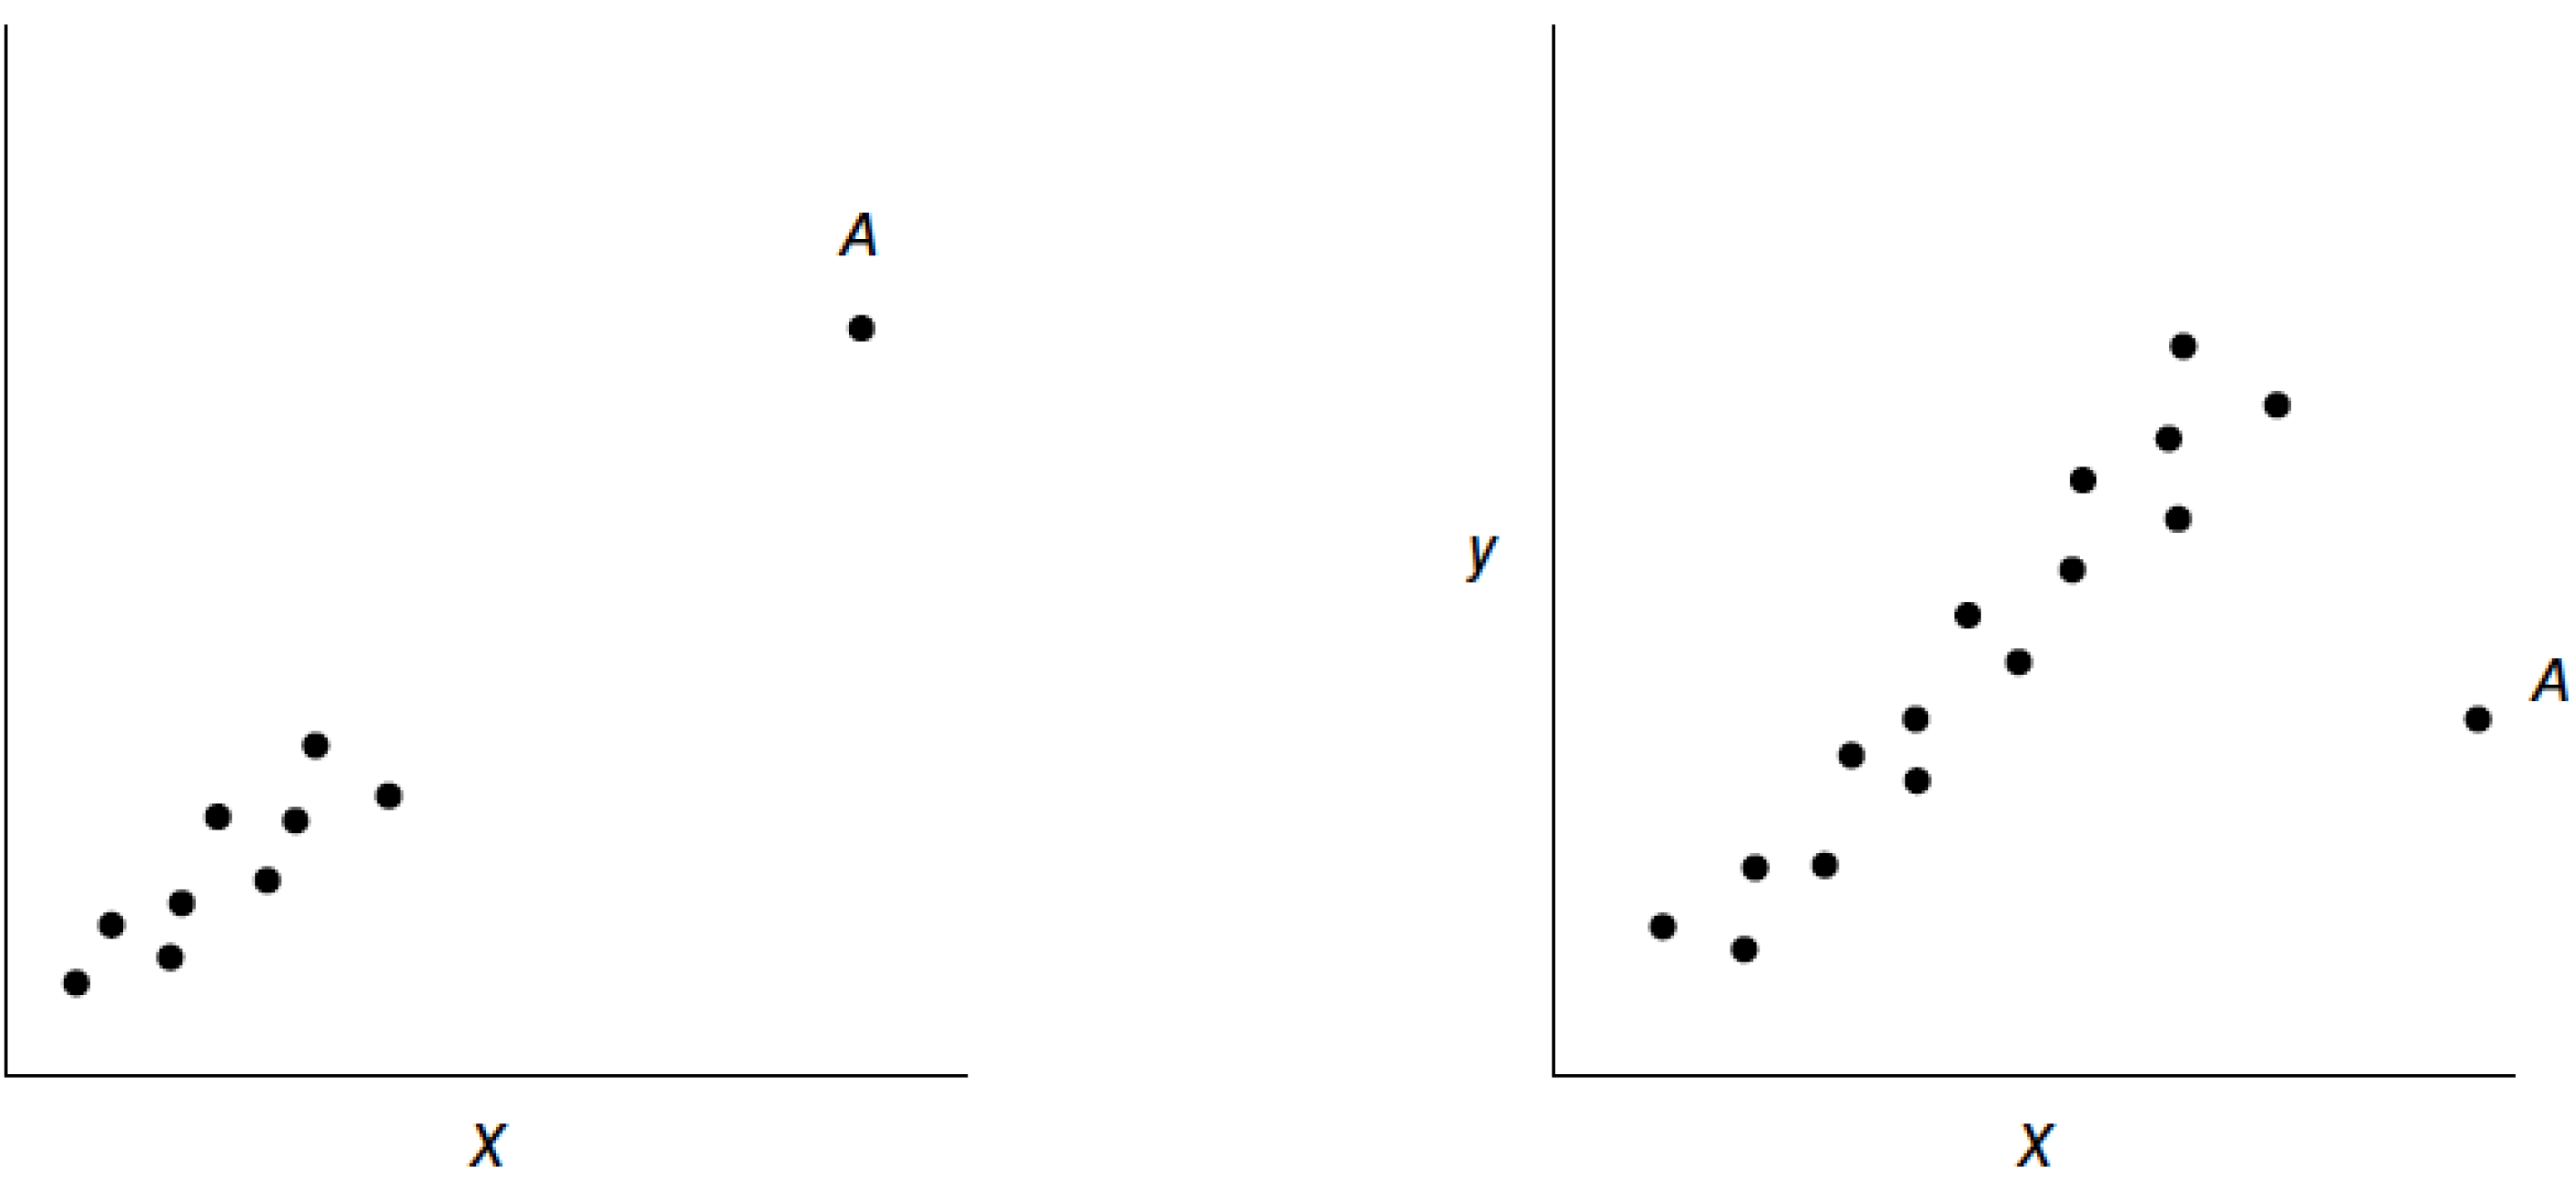
\includegraphics[scale=.22]{figs8/Leverage_Influence.png} 
%
%
%\end{frame}
%
%
%
%
%\begin{frame}{  Cook's Distance to Detect Influential Points }
%\qBrd[4.5in]{gray!30}{ \sqBullet{orange} { Standardized Residual residual:} \tiny   $\HLTY{\HLTW{z_i} := \frac{\hat{Y}_i-Y_i}{\hat{\sigma} }}$
%{\tiny: Based on the linear regression assumptions, we might expect the $z_i$'s to resemble a sample from a N(0, 1) distribution.}
%}\\
%\vspace{.01in}
%
%\qBrd[4.5in]{gray!30}{ \sqBullet{violet}  { Studentized Residual:} It is defined to be  \tiny $\HLTY{\HLTW{e_i} := \frac{\hat{Y}_i-Y_i}{\hat{\sigma}\sqrt{ \HLTEQ[lime]{1-h_{_{i,i}} }  }}}$. {\tiny: approximately follows a t
%distribution with $n - p$  degrees of freedom (under the standard assumptions of the SLR).  In large data sets (large n), the standardized
%and studentized residuals should not differ dramatically.}
%}\\
%\vspace{.01in}
%
%\qBrd[4.5in]{gray!30}{ \sqBullet{violet} {Cook's Distance:} \tiny $$\HLTY{\text{CD}_i:= \frac{\HLTW{e_i^2} }{p} \frac{h_{_{i,i}} }{1-h_{_{i,i}} }} .$$
%}
%
%\vspace{.1in}
%\qBrd[4.5in]{green!30}{
%{\bf 
%It is suggested to examine the cases with $\text{CD}_i > 0.5$ and that
%cases with $\text{CD}_i > 1$ can be highly influential. }}
%\end{frame}
%
%
%
%%
%%\begin{frame}{  Leverage and Influence }
%%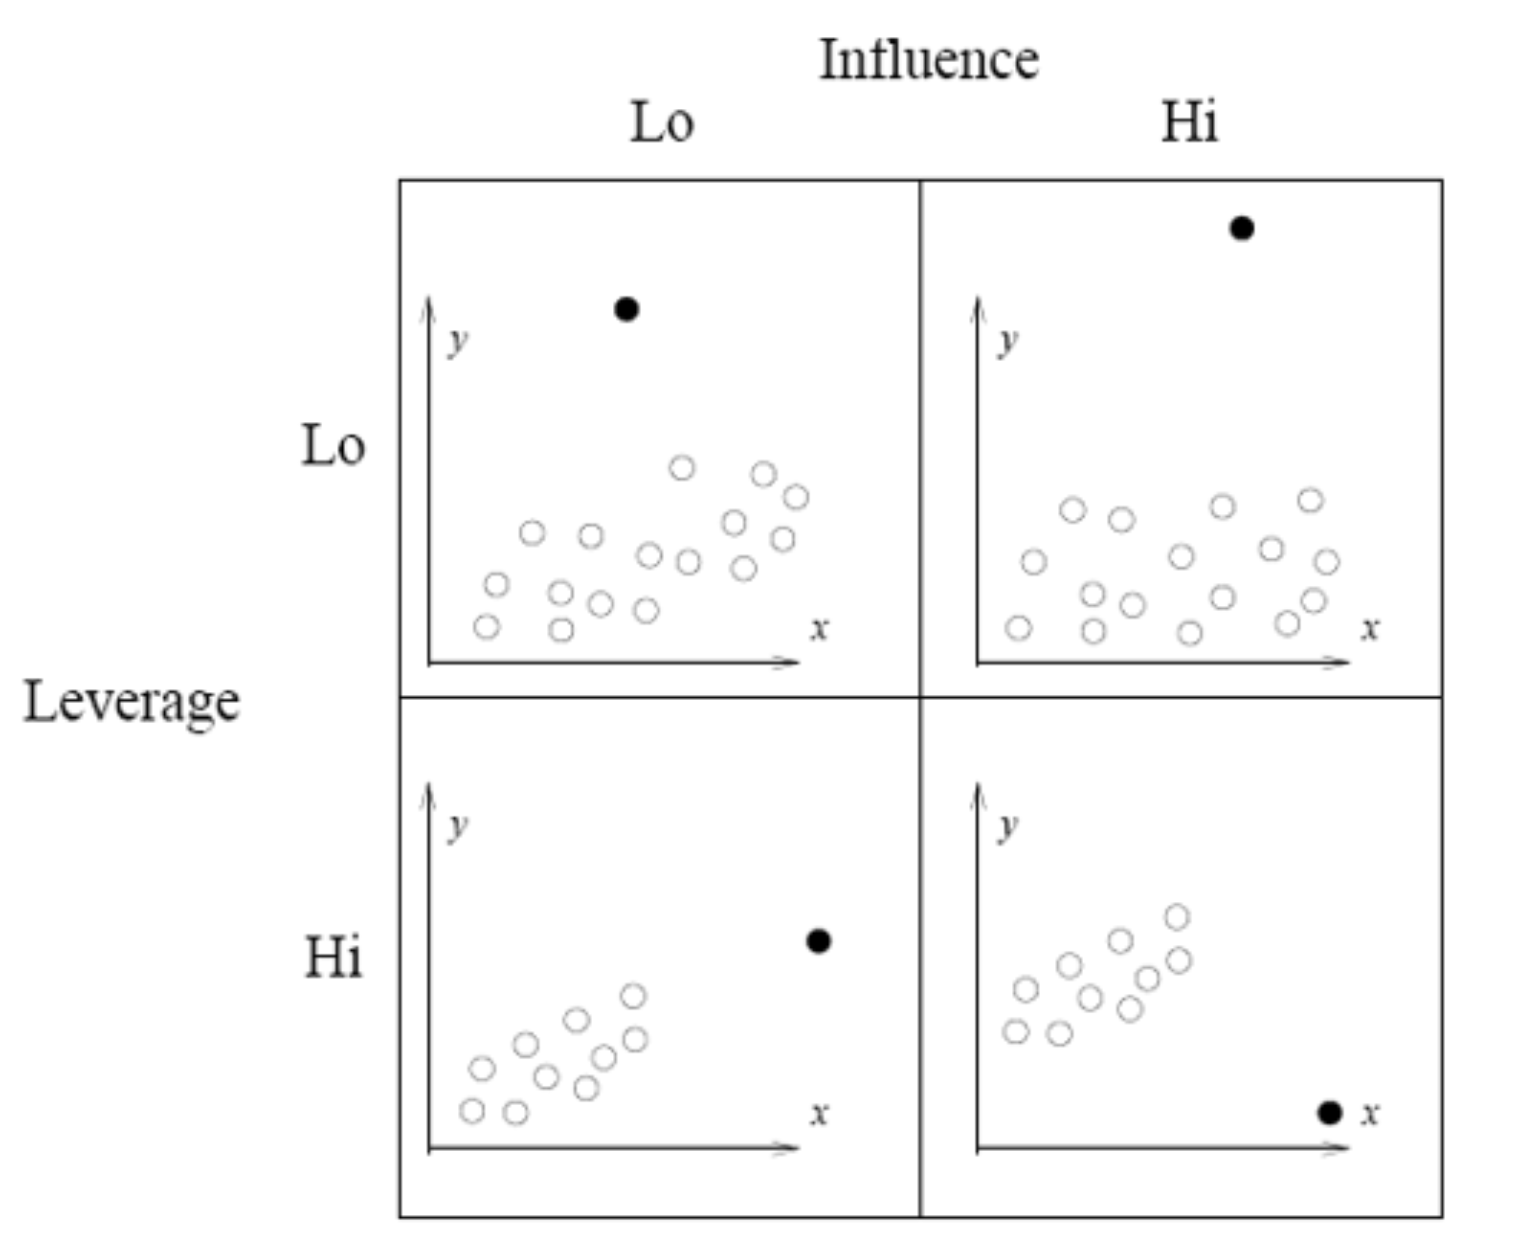
\includegraphics[scale=.35]{figs8/Inf_lev.png} 
%%
%%
%%\end{frame}
%
%
%
%
%
%
%\TransitionFrame[antiquebrass]{\Large Residual  Plots}
%
%
%\begin{frame}{ A Typical Desirable Residual Plot   }
%\qBrd{blue!30}{{\bf Residual Plot:} Graph of Residuals against Predictor variable or
%against the fitted values is helpful to see if the
%variance of error terms are constant. 
%}
%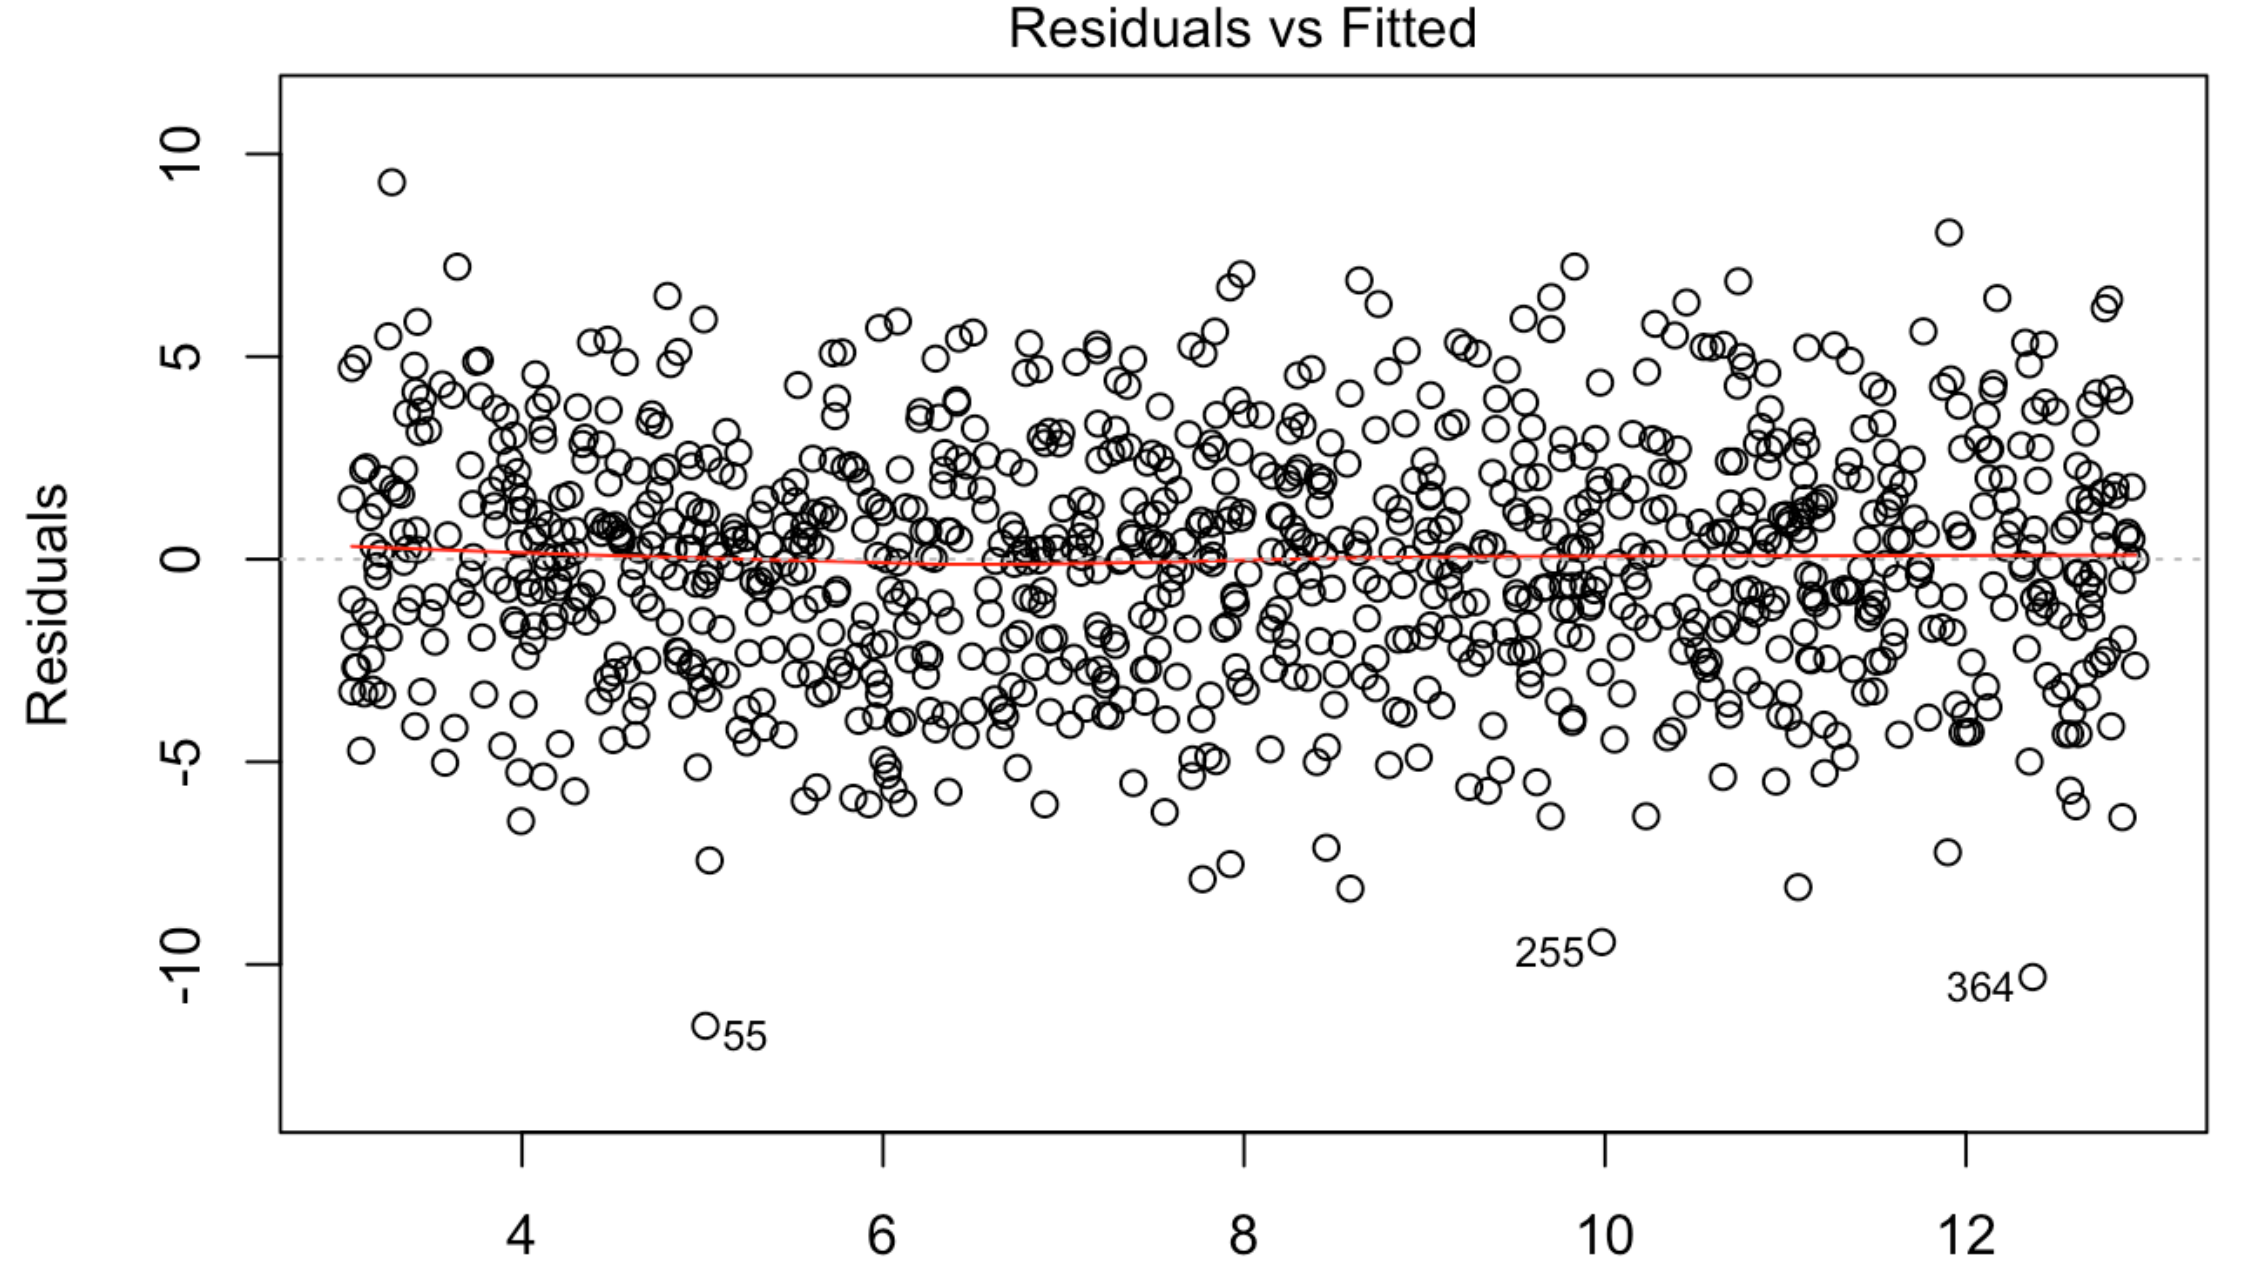
\includegraphics[scale=.3]{figs8/IdealResidual.png} 
%
%
%\end{frame}
%
%
%\begin{frame}{   Residual  Plots }
%
%\qBrd[4.6in]{violet!30}{ 
%\sqBullet{violet}The plots of the residuals, Studentized Residual and Standardized residuals can be utilized to visually identify  key insights, not only  in identifying influential points, but also many additional information. regarding the regression diagnostics. }
%\end{frame}
%
%
%
%
%
%
%
%
%
%
%\TransitionFrame[antiquebrass]{\Large Detection for Lack of Normality of Residuals:\\  Shapiro-Wilk's Test for Residuals}
%
%
%\begin{frame}{ Normal Q-Q Plot }
%
%\qBrd[4.5in]{blue!30}{  {\bf Normal Q-Q Plot:} Theoretical quantiles (percentiles) from the standard normal distribution are plotted against the empirical quantiles of the standardized residuals. 
%}\\
%\vspace{.2in}
%
%\qBrd[4.5in]{green!30}{ In ideal scenario, when there is no model assumptions violation on normality of the residuals,  all the points on a Normal Q-Q plot for the standardized residuals should be on the (very close to the) X=Y straight line.
%}\\
%
%
%\end{frame}
%
%
%
%
%
%\begin{frame}{  Examples: Q-Q Plots  }
%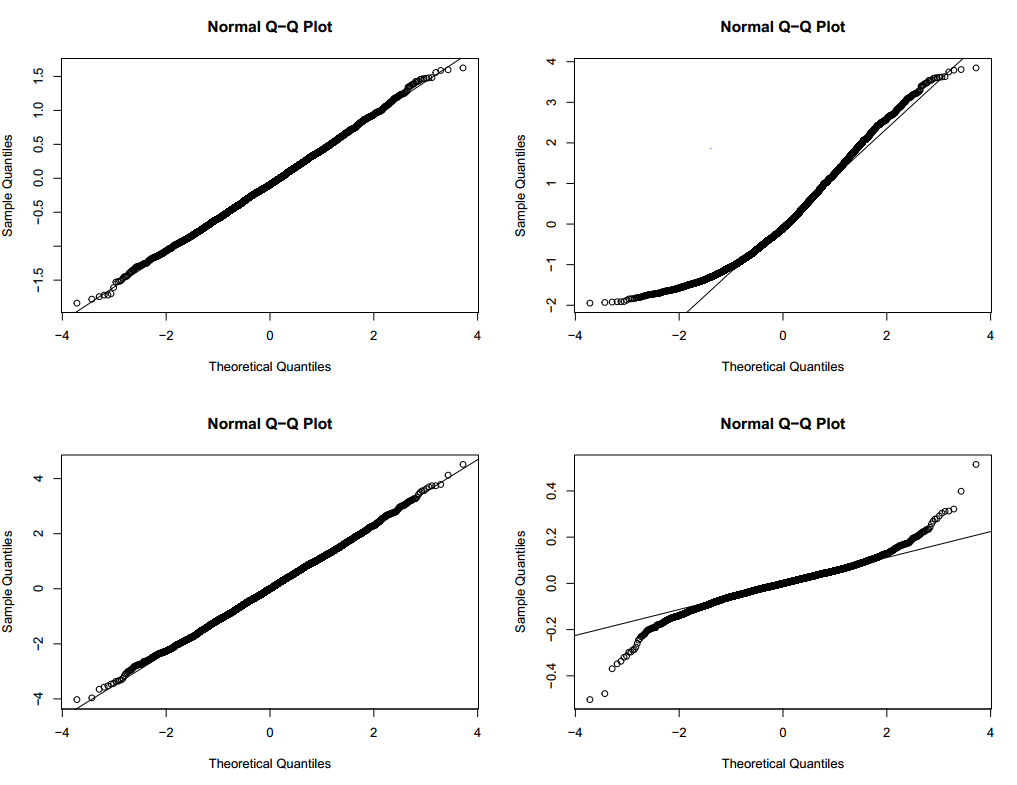
\includegraphics[scale=.3]{figs8/qq_examples.png} 
%
%
%\end{frame}
%
%
%
%\begin{frame}{  Statistical Test of Normality for Residuals: Shapiro-Wilk test  }
%
%\begin{center}
%\qBrd{blue!30}{
%It tests for whether the errors/residuals are Normally distributed or nor. 
%\vspace{-.2in} \begin{center}
%\qBrd[2in]{slateblue!50}{$H_0: \text{\tiny Residuals are Normaly Distributed}\\ \text{ vs } \\H_1: \text{ \tiny Residuals are not Normaly Distributed } \vspace{-.01in}$}
%\end{center}
%}
%%\qBrd[4.5in]{gray!30}{ \tiny Define: $e^{*}_{i}:= \hat{Y}_i - Y_i.$ .  Let $e^{*}_{(1)}< e^{*}_{(2)} < \ldots < e^{*}_{(n)}$ are the ordered values of residuals.  }
%%\qbx{gray!40}{ $$Test Statistic= \DBX{W= \frac{\sum_{i=1}^{n} a_ie^{*}_{(i)} }{ \sum_{i=1}^{n} \left( e^*_i - \bar{e}^* \right)^2} \text{  where } \bar{e}^* } = \frac{1}{n}\sum{e^*_i}. $$
%%}
%%\\
%%
%%\vspace{-.2in}
%%\qBrd[4.5in]{slateblue!50}{ $a_1, a_2, \ldots, a_n$ are appropriately chosen numbers related to the joint distribution of n ordered standard normal random variables.  {\tiny Specifically ${\bf a}:= \frac{m^T V^{-1}}{\vert m^T V^{-1}\vert }$}  }\\
%
%
%\end{center}
%
%
%\end{frame}
%
%%
%%\begin{frame}{  Statistical Test of Normality for Residuals: Shapiro-Wilk test  }
%%
%%\begin{center}
%%\qBrd{blue!30}{
%%It tests for whether the errors/residuals are Normally distributed or nor. 
%%\vspace{-.2in} \begin{center}
%%\qBrd[2in]{slateblue!50}{$H_0: \text{\tiny Residuals are Normaly Distributed}\\ \text{ vs } \\H_1: \text{ \tiny Residuals are not Normaly Distributed } \vspace{-.01in}$}
%%\end{center}
%%}
%%\qBrd[4.5in]{teal!30}{ Define: $e^{*}_{i}:= \hat{Y}_i - Y_i.$ .  Let $e^{*}_{(1)}< e^{*}_{(2)} < \ldots < e^{*}_{(n)}$ are the ordered values of residuals.  }
%%\qbx{violet!40}{ $$Test Statistic= \DBX{W= \frac{\sum_{i=1}^{n} a_ie^{*}_{(i)} }{ \sum_{i=1}^{n} \left( e^*_i - \bar{e}^* \right)^2} \text{  where } \bar{e}^* } = \frac{1}{n}\sum{e^*_i}. $$
%%}
%%\\
%%
%%\qBrd[4.5in]{slateblue!50}{ $a_1, a_2, \ldots, a_n$ are appropriately chosen numbers related to the joint distribution of n ordered standard normal random variables.  {\tiny Specifically ${\bf a}:= \frac{m^T V^{-1}}{\vert m^T V^{-1}\vert }$ where m, V be the mean and variance of the n ordered standard normal random variables.  }   }\\
%%
%%
%%
%%\end{center}
%%
%%
%%\end{frame}
%%
%
%
%
%
%
%\begin{frame}{  Statistical Test of Normality for Residuals: Shapiro-Wilk test  }
%
%\begin{center}
%\qBrd{blue!30}{
%It tests for whether the errors/residuals are Normally distributed or nor. 
%\vspace{-.2in} \begin{center}
%\qBrd[2in]{slateblue!50}{$H_0: \text{\tiny Residuals are Normaly Distributed}\\ \text{ vs } \\H_1: \text{ \tiny Residuals are not Normaly Distributed } \vspace{-.01in}$}
%\end{center}
%}\\
%\vspace{.1in}
%\qBrd[4.5in]{gray!50}{The test statistic is Denoted as W. $0<W\leq 1$.  $W$ is a fraction.  } \\
%\vspace{.1in}
%
%
%\qBrd[4.5in]{gray!50}{ Decision: We have strong statistical evidence to Reject the Null Hypothesis if the corresponding p-value is less than .05.    }
% \\
%\vspace{.1in}
%
%\qBrd[4.5in]{green!50}{ If Assumption of normality are true : the  p-value is {\bf  more then  .05} then there is no statistical evidence to believe that the residuals are not Normally distributed.    }
%
%\end{center}
%
%
%\end{frame}
%
%\definecolor{airforceblue}{rgb}{0.36, 0.54, 0.66}
%\TransitionFrame[airforceblue]{\Large A Possible Remedy to Deal with Non-Normality of the Residuals.    }
%
%
%
%
%\begin{frame}{  Box-Cox Power  Transformation of the Responses }
%
%The power transformation is parametrized by $\lambda $ (a real value can be positive negative or zero.)
%\begin{center}
%\qBrd{blue!30}{\begin{center}
%\DBX{ \tilde{Y} = 
%\begin{cases}
%\log(Y) & \text{ if } \lambda=0\\
%\frac{Y^{\lambda}-1}{\lambda} &\text{ if } \lambda\neq 0\\
%\end{cases} }\end{center}
%}\\
%\vspace{.1in}
%\qBrd[4.5in]{violet!50}{\sqBullet{violet}Optimal $\lambda$ is often estimated by a cross validation procedure.  Standard Statistical software typically provide a procedure to identify its optimal value. } \\
%\vspace{.1in}
%\qBrd[4.5in]{lime!50}{ \sqBullet{green} Box-Cox Transformation may resolve the issues due to the non normality of the residuals and heteroscedasticity. } \\
%\vspace{.1in}
%
%
%\end{center}
%
%
%\end{frame}
%
%
%\definecolor{armygreen}{rgb}{0.29, 0.33, 0.13}
%
%\TransitionFrame[armygreen]{\Large  Detection of  heteroscedasticity (Non constant $\sigma^2$)}
%
%
%
%\begin{frame}{ Identification of non-constant Error Variance   }
%\qBrd{blue!30}{{\bf Residual Plot:} Graph of Residuals against Predictor variable or
%against the fitted values is helpful to see if the
%variance of error terms are constant. 
%}
%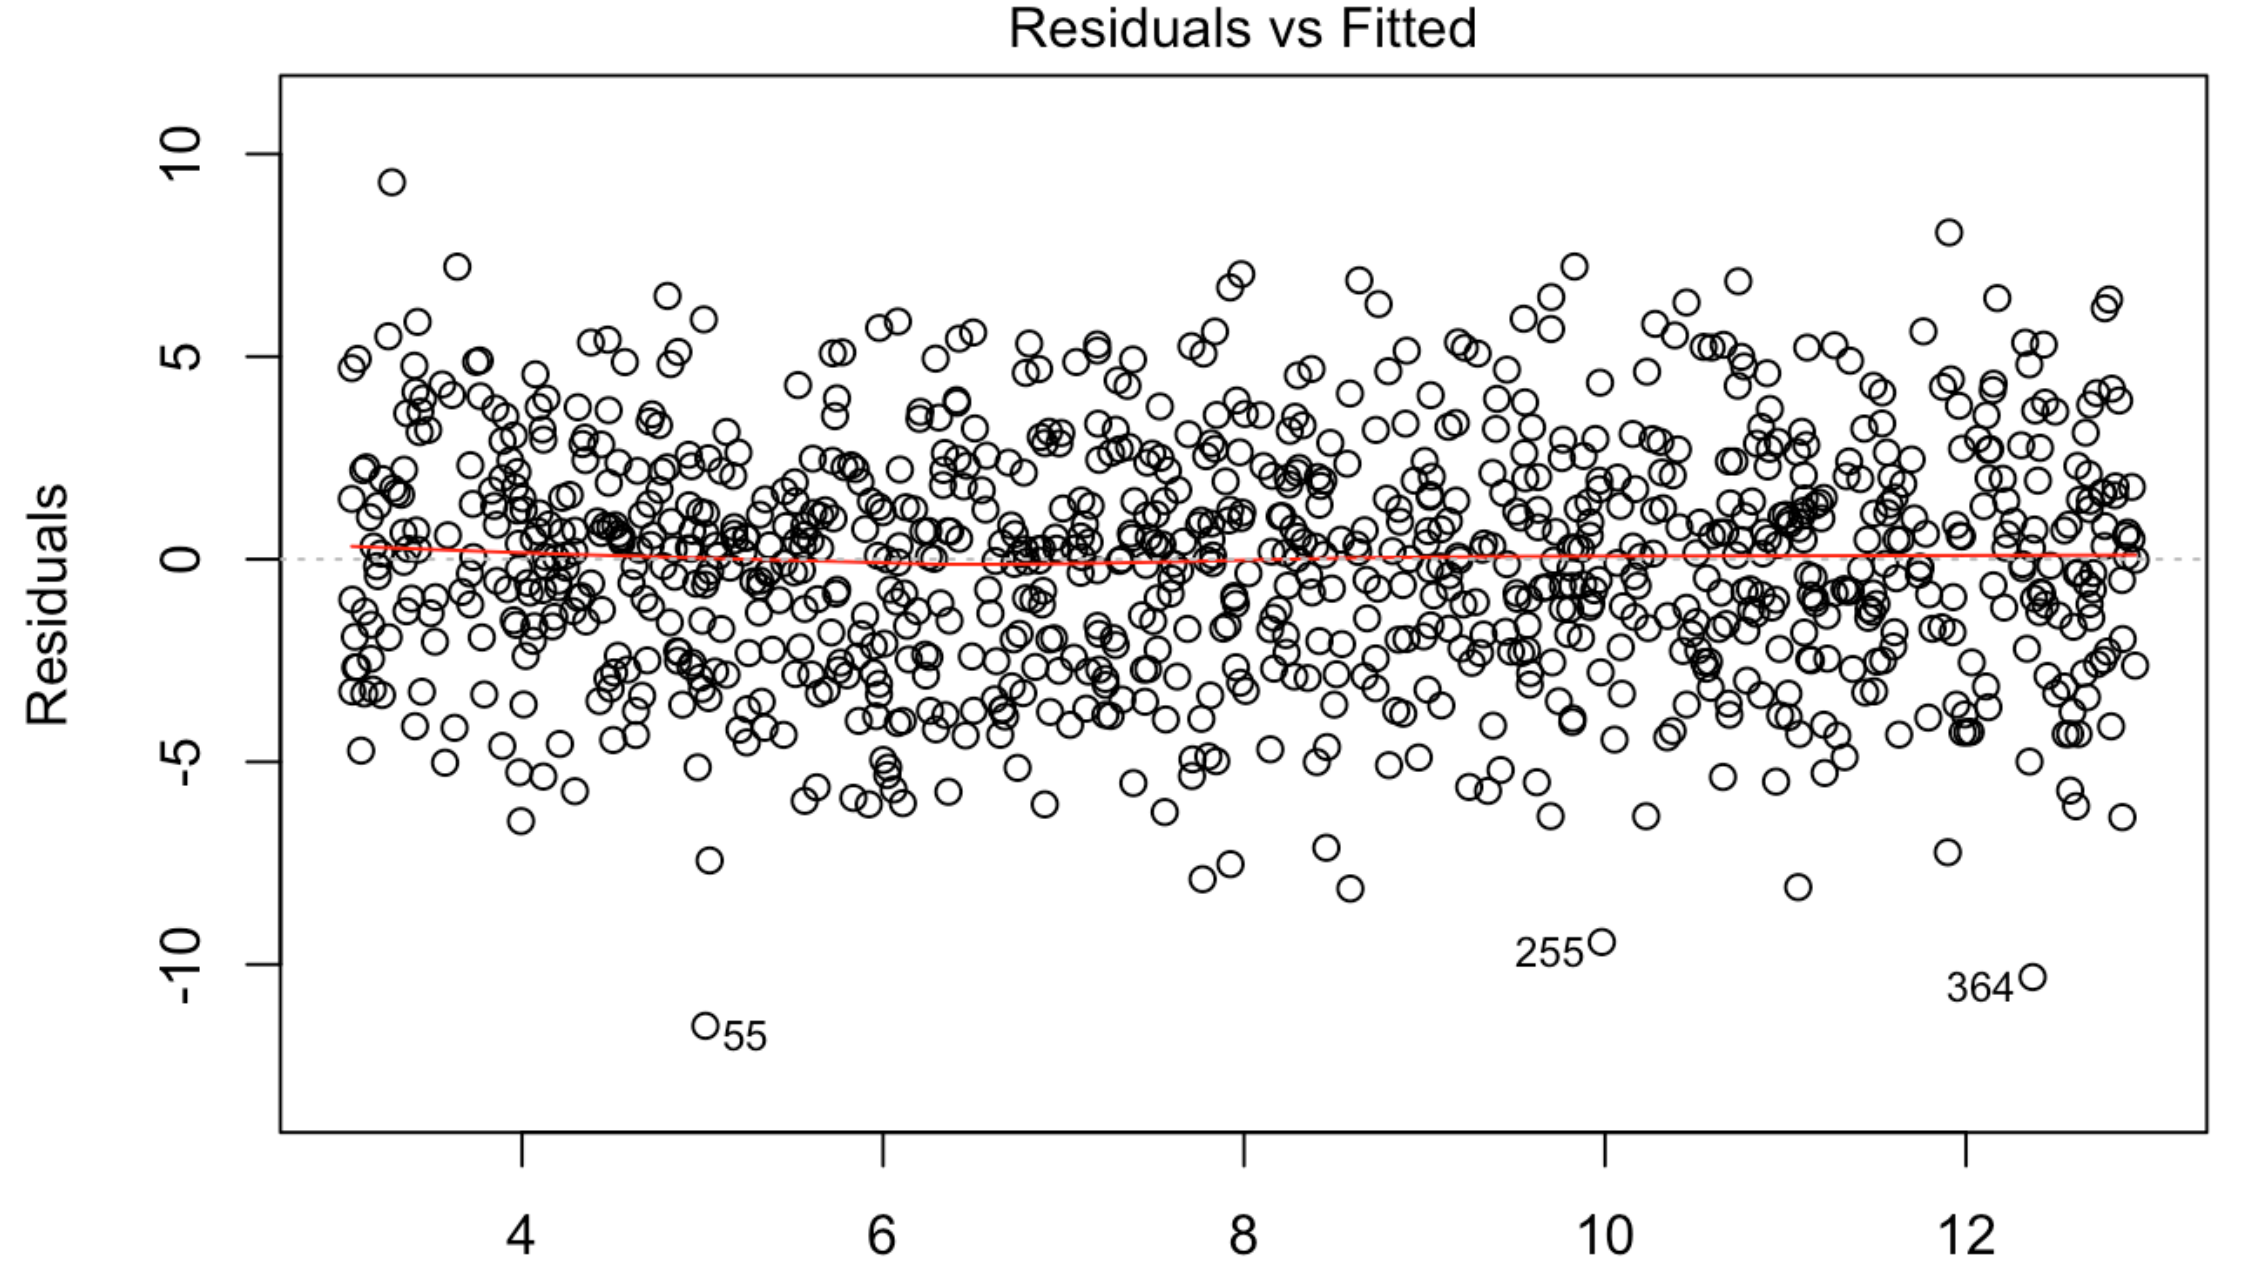
\includegraphics[scale=.3]{figs8/IdealResidual.png} 
%
%
%\end{frame}
%
%
%
%\begin{frame}{ Identification of non-constant Error Variance   }
%\qBrd{blue!30}{{\bf Residual Plot:}  Variability of the residuals appears to be increasing.
%}
%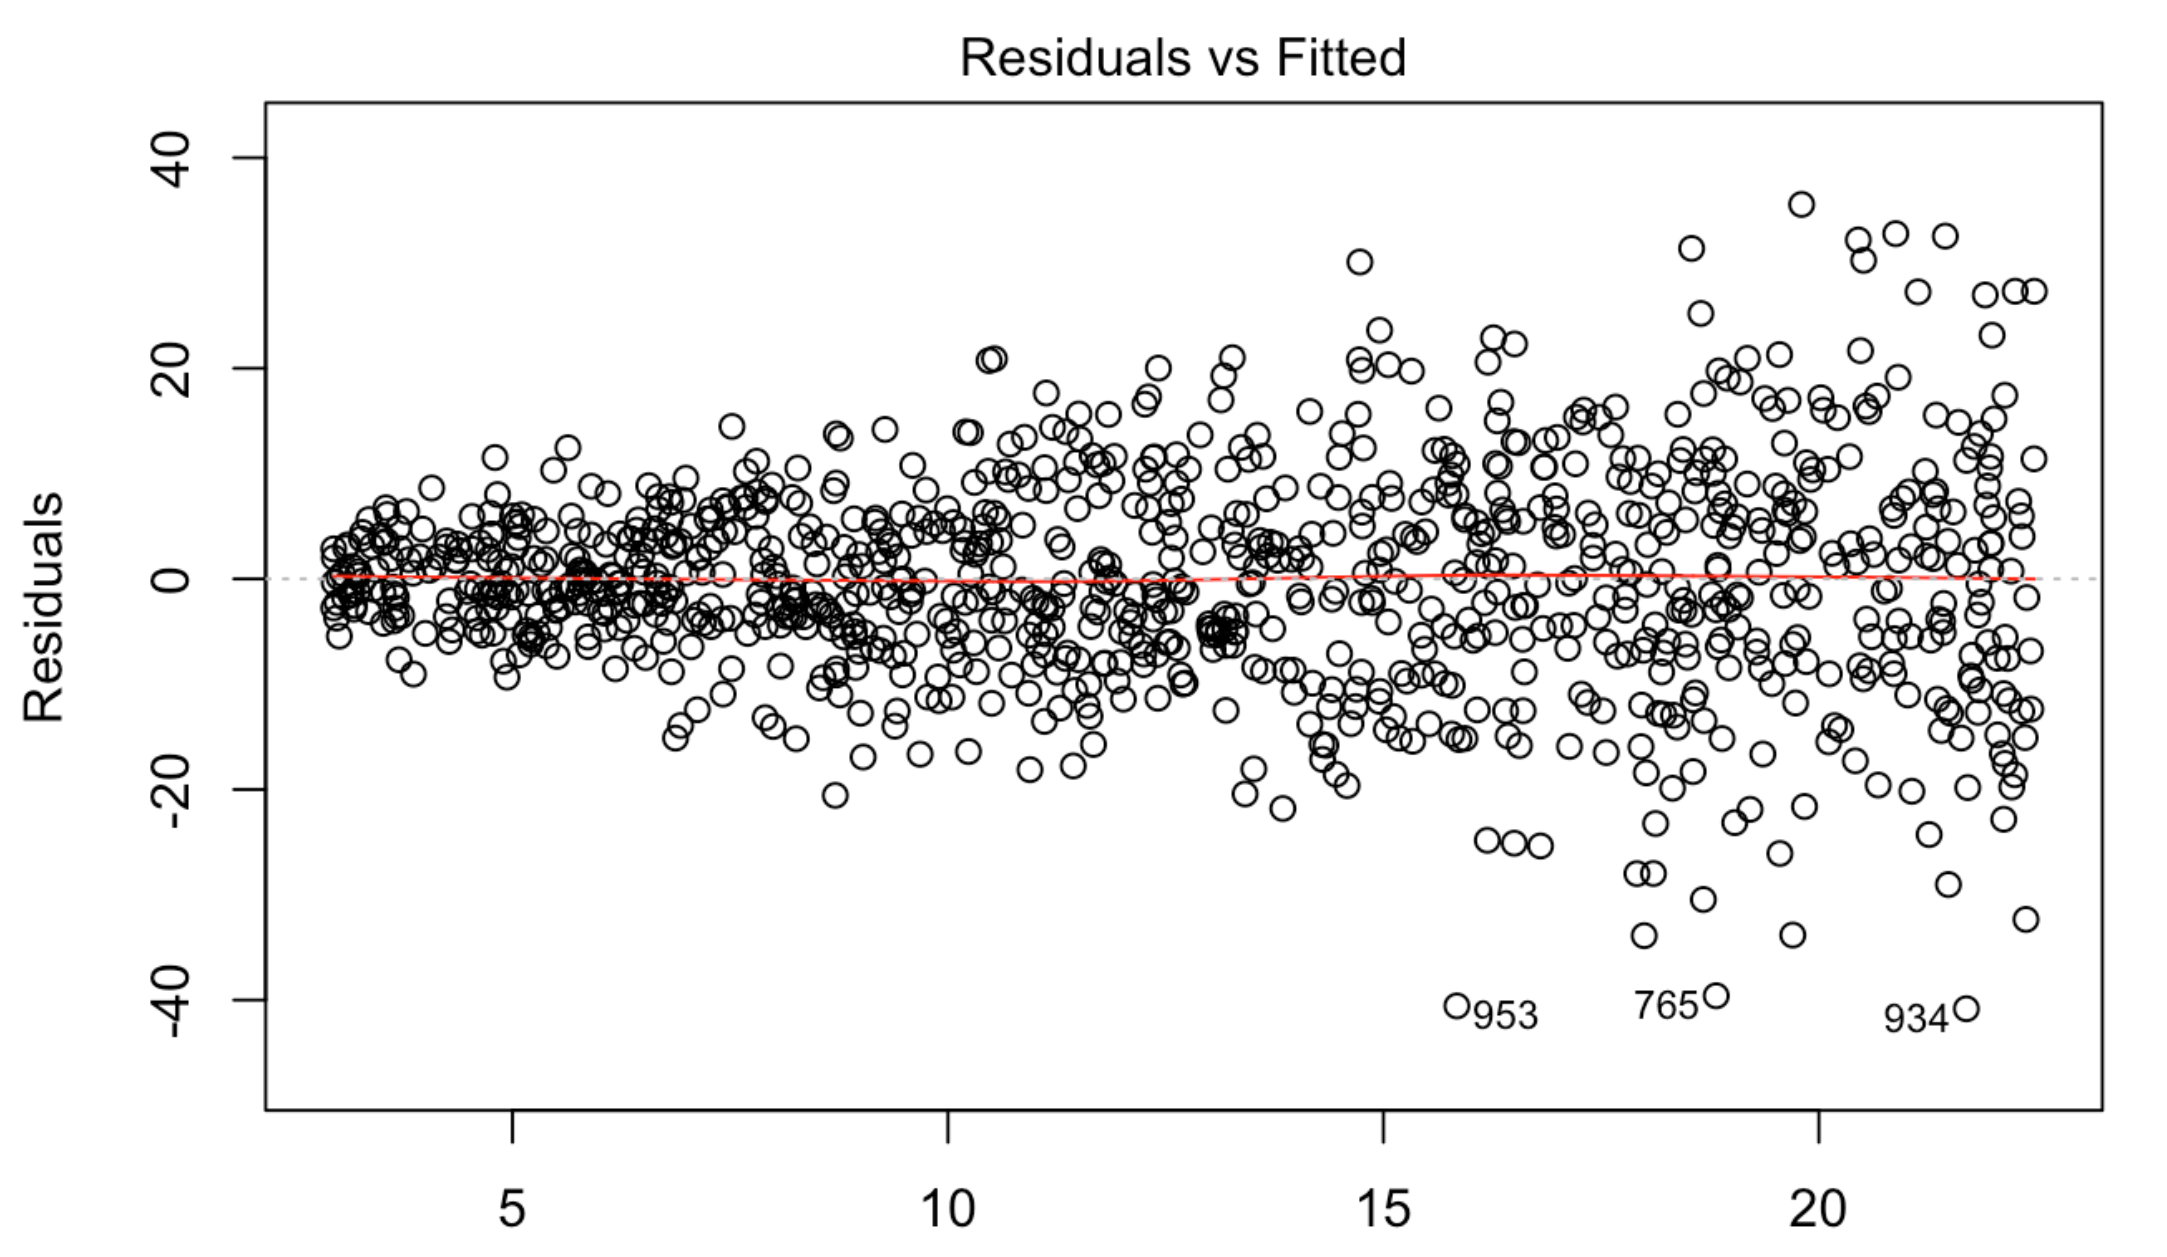
\includegraphics[scale=.3]{figs8/varIncrease.png} 
%
%
%\end{frame}
%
%
%
%
%
%
%\begin{frame}
%\qBrd{airforceblue!50}{ \sqBullet{airforceblue} A Possible remedy to deal with non constant variability is to utilize weighted Least Square. }
%
%\qBrd{green!20}{ \sqBullet{airforceblue} Use appropriate transformation on the Responses (Y).}
%\end{frame}
%
%
%
%
%
%
%
%
%\TransitionFrame[antiquebrass]{\Large  Detection of Correlated Model Errors ($\varepsilon_i$): \\ Durbin-Watson Test}
%
%
%
%\begin{frame}{ Identification of Non Linearity  }
%\qBrd{blue!30}{{\bf Residual Plot:}  Violation of the Linearity Assumption. The errors are not statistically independent/uncorrelated.  There seem to be  a seasonality.
%}
%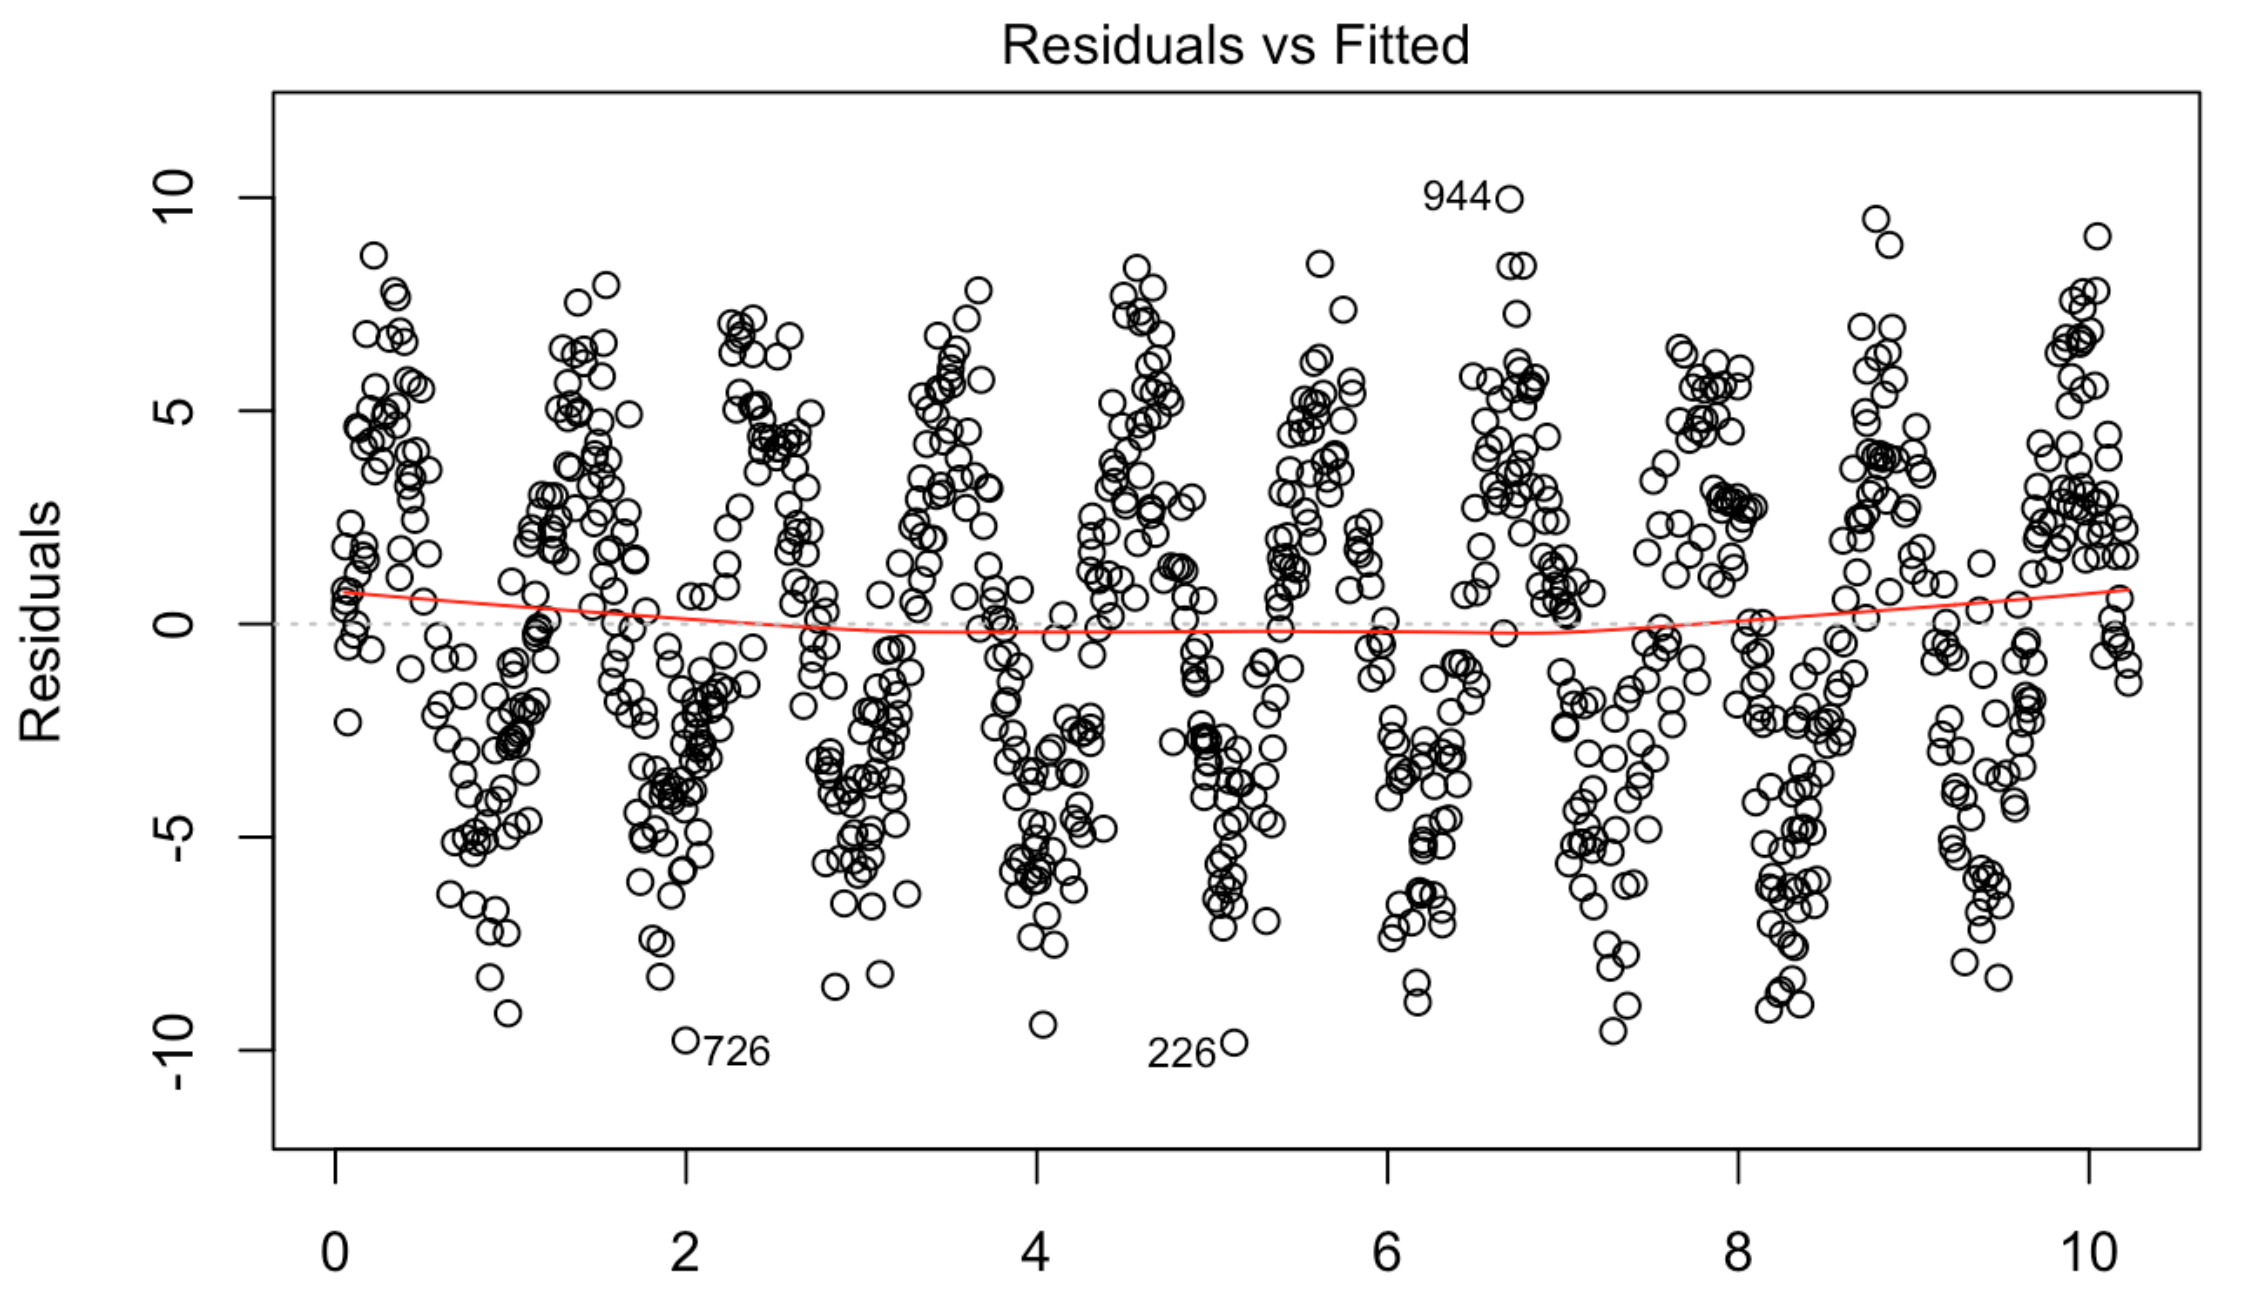
\includegraphics[scale=.28]{figs8/Seasonal.png} 
%
%
%\end{frame}
%
%\begin{frame}{ Darbin Watson Test (DW Test) for identifying Correlated Model Errors }
%\vspace{-.05in}
%\begin{center}
%\qBrd{blue!30}{
%It tests for whether the errors/residuals are auto-correlated or not.  Let $\rho$ denotes the lag 1 auto correlation between the errors.   i.e.  If $\text{corr}( \varepsilon_i,  \varepsilon_{i-1})= \rho$ then it tests for\\
%\vspace{-.2in} \begin{center}
%\qBrd[3in]{slateblue!50}{$$H_0: \rho= 0 \text{ vs } H_1: \rho\neq 0 \vspace{-.1in}$$}
%\end{center}
%}
%
%\qBrd[2in]{olive!50}{ \tiny Define: $e^{*}_{i}:= \hat{Y}_i - Y_i.$ }
%\qbx{violet!40}{ \tiny $Test Statistic= d= \frac{\sum_{i=1}^n\left(e^{*}_{i}- e^{*}_{i-1}\right)^2}{\sum_{i=1}^n{e^{*}}^2}$
%}
%
%\vspace{-.1in}
%\qBrd[4.5in]{gray!50}{ Reject Null Hypothesis if $d$ is large or small.  `significantly large' value of d indicates negative correlation,  `significantly small' values of d is indicative of positive correlation   }
%
%
%
%\qBrd[4.5in]{green!50}{ Assumption are met (errors are not correlated ): If the corresponding p-value of the test is LARGER than .05 }
%
%
%
%\end{center}
%\end{frame}
%
%\begin{frame}
%\qBrd{airforceblue!50}{ \sqBullet{airforceblue} A Possible remedy is to use  utilize Time series models such as AR, ARMA, ARIMA, GARCH model. Uf there is seasonality in the model try to include some periodic function along with the linear functions.  }
%\end{frame}
%
%
%
%\TransitionFrame[antiquebrass]{\Huge Thank You}
%
\TransitionFrame{THANK YOU}

\section{Example: O-Ring Failure Data}


\begin{frame}{Example: Analysis of the O ring Failure Data}
	\vspace{-3mm}

  \qBrd[4.2in]{teal!35}{  \sqBullet{teal} The Space Shuttle Challenger crashed 73 seconds after liftoff on January 28th, 1986. The disaster claimed the lives of all seven astronauts on board. The details surrounding this disaster were very involved. } \\
  \vspace{.1in}
  \qBrd[4.3in]{orange!40}{
  \sqBullet{purple}  If you are interested in learning more, watch this 18-minute video documentary on
  {\color{blue}\href{https://www.pbs.org/video/retro-report-on-pbs-season-1-episode-7-lessons-space-shuttle-challenger-tragedy/}{PBS.org}}.
 }\\
 \vspace{.1in}
  \qBrd[4.3in]{olive!40}{\sqBullet{olive} 
  "The engineers who manufactured the large boosters that launched the rocket had data on the possible failures that could happen during cold temperatures. They tried to prevent the launch, but were ultimately ignored and disaster ensued."}
	

\end{frame}




\begin{frame}{Context: Analysis of the O ring Failure Data}
	\vspace{-3mm}

  \qBrd[4.2in]{teal!35}{  \sqBullet{teal} It was known that there is an association between the  O-Ring seal failure and the low atmosphere temparature temperature. } \\
  \vspace{.1in}
 
  \qBrd[4.3in]{purple!40}{\sqBullet{purple} 
  The ``fail" column in the data set below records how many O-rings experienced failures during that particular launch. The ``temp" column lists the outside temperature at the time of launch.}
	

\end{frame}



\begin{frame}{Model}
	\vspace{-3mm}

  \qBrd[4.2in]{teal!35}{ 
  The seven rows of the Data is:\\
  \begin{center}
  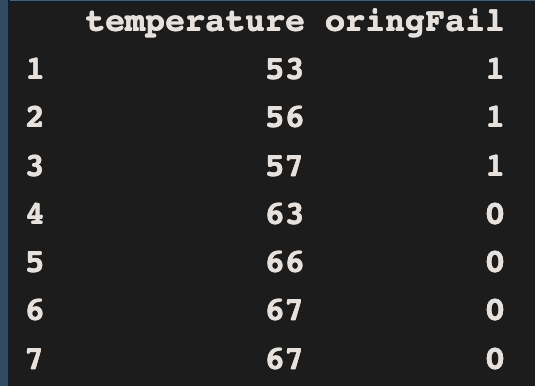
\includegraphics[scale=.5]{oringData.png} 
  \end{center}
  } \\
  

\qbx[4.5in]{purple!40}{ 
Model: \\
\qBrd[2in]{babyblue!40}{$\pi_i=Prob(\text{oringFail}_i=1)$}\\
\qBrd[3in]{teal!50}{ $\Logit{\pi_i}=\HLTY{\beta_0} +\beta_1\text{temparature}_i$} 
 }\\
 
 \end{frame}
 
 
\begin{frame}{Code}


  \qBrd[4.7in]{teal!35}{ 
  \begin{center}
  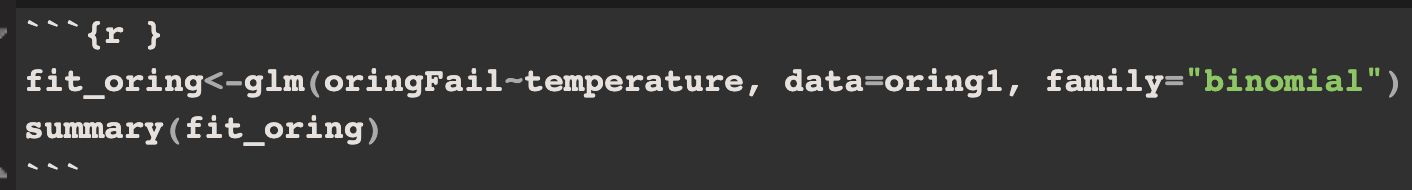
\includegraphics[scale=.48]{oringCode.png} 
  \end{center}
  } 
  \end{frame}
  
  \begin{frame}{Output}
   \qBrd[4.7in]{blue!35}{ 
  \begin{center}
  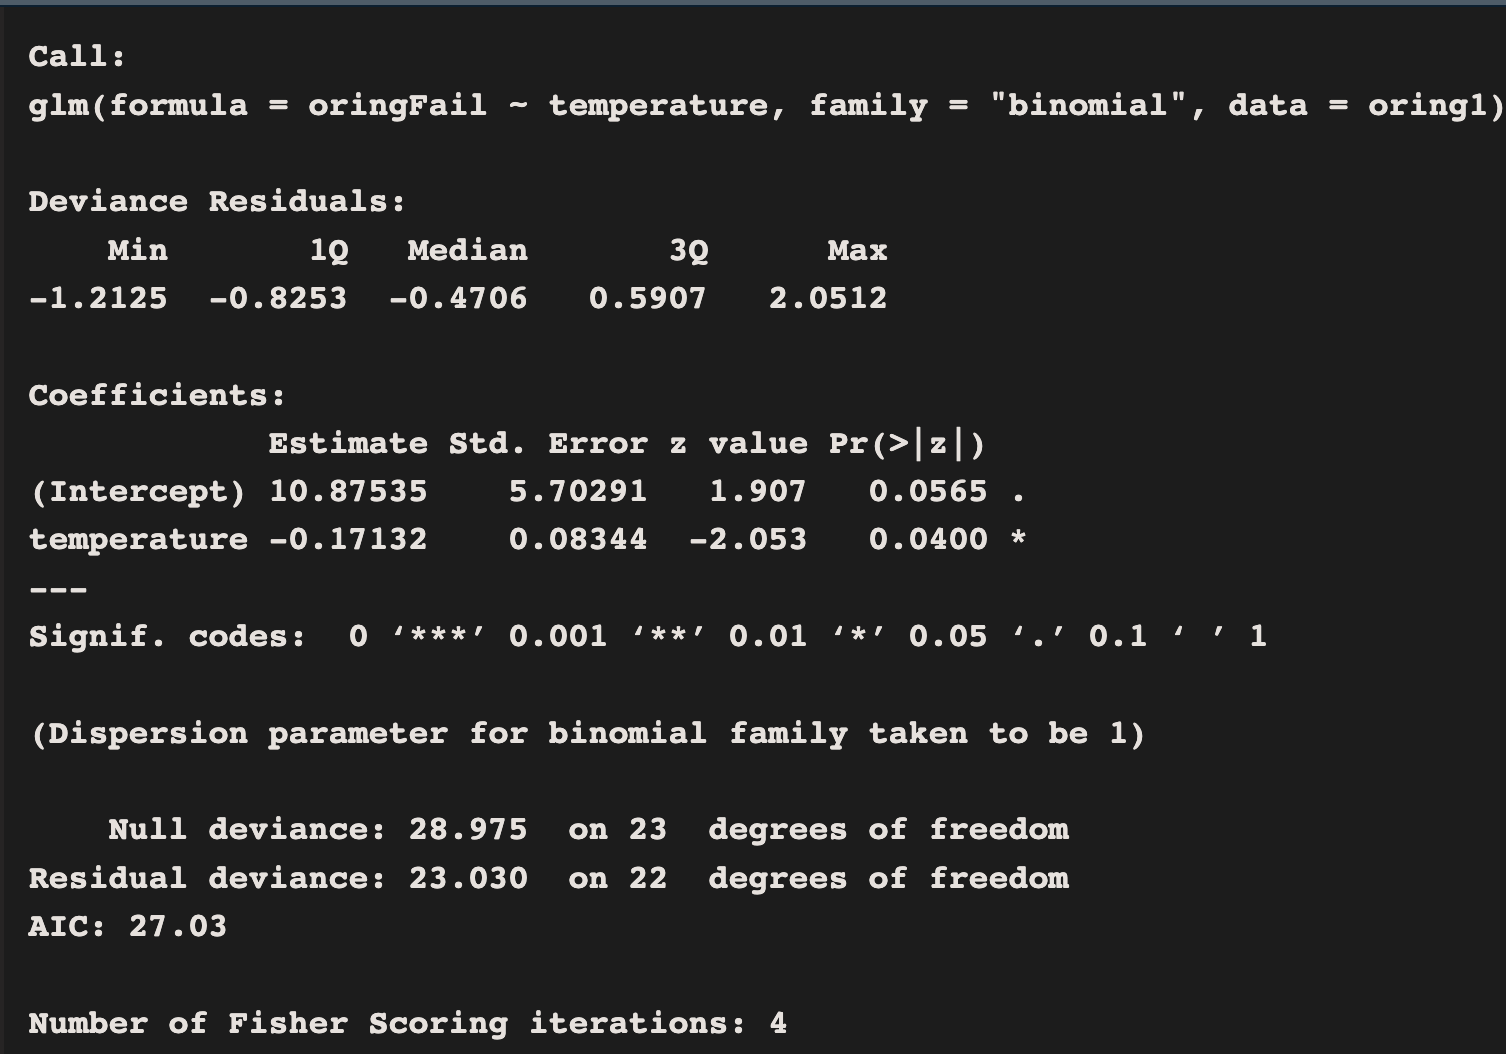
\includegraphics[scale=.4]{oringOutput.png} 
  \end{center}
  } 
  
  \end{frame}
  
  
  

\begin{frame}{Model}
	\vspace{-3mm}

 

\qbx[4.5in]{purple!40}{ 
Fitted Model: \\
\qBrd[2in]{babyblue!40}{$\pi_i=Prob(\text{oringFail}_i=1)$}\\
\qBrd[3in]{teal!50}{ $\Logit{\pi_i}=\HLTY{\hat{\beta}_0} +\hat{\beta}_1\text{temparature}_i$} 
 }\\
 \vspace{2in}
 
 \end{frame}
 
 
\begin{frame}{Interpret the Intercept}


 

 
 \end{frame}
 
 
\begin{frame}{Interpret the regression coefficient corresponding to the temparature}


 

 
 \end{frame}
 
  
 
 
\begin{frame}{Prediction}
	\vspace{-3mm}

 

\qbx[4.5in]{orange!40}{ 
The actual temperature at the Challenger launch was 31 F.\\
Predict the Probability of Failure.
 }\\
 \vspace{2.5in}
 
 \end{frame}
 
 
 

\begin{frame}{Comment}
	\vspace{-3mm}

 

\qbx[4.5in]{purple!40}{ 
It is interesting to note that all of these data were available
prior to launch. However, engineers were unable to effectively
analyze the data and use them to provide a convincing
argument against launching Challenger to NASA managers.
 }\\

 
 \end{frame}






\begin{frame}{Example:  Can Logistic Regression separates "Apples" from the "Oranges"?}
	
  \qBrd[4.2in]{teal!35}{
  \begin{center}
   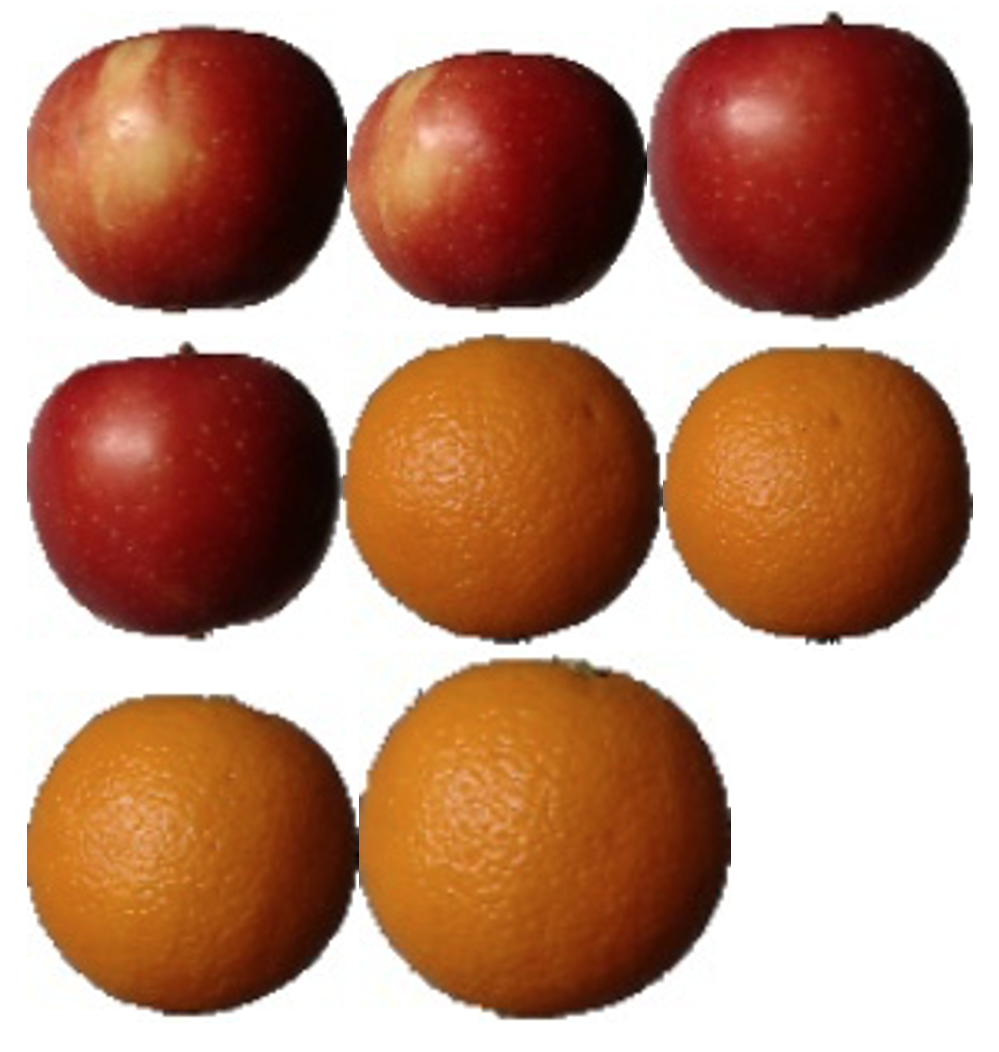
\includegraphics[scale=.35]{ApplesOranges.png} 
   \end{center}
  } \\
  

\end{frame}


\begin{frame}{How about this?}
	
  \qBrd[4.2in]{teal!35}{
  \begin{center}
   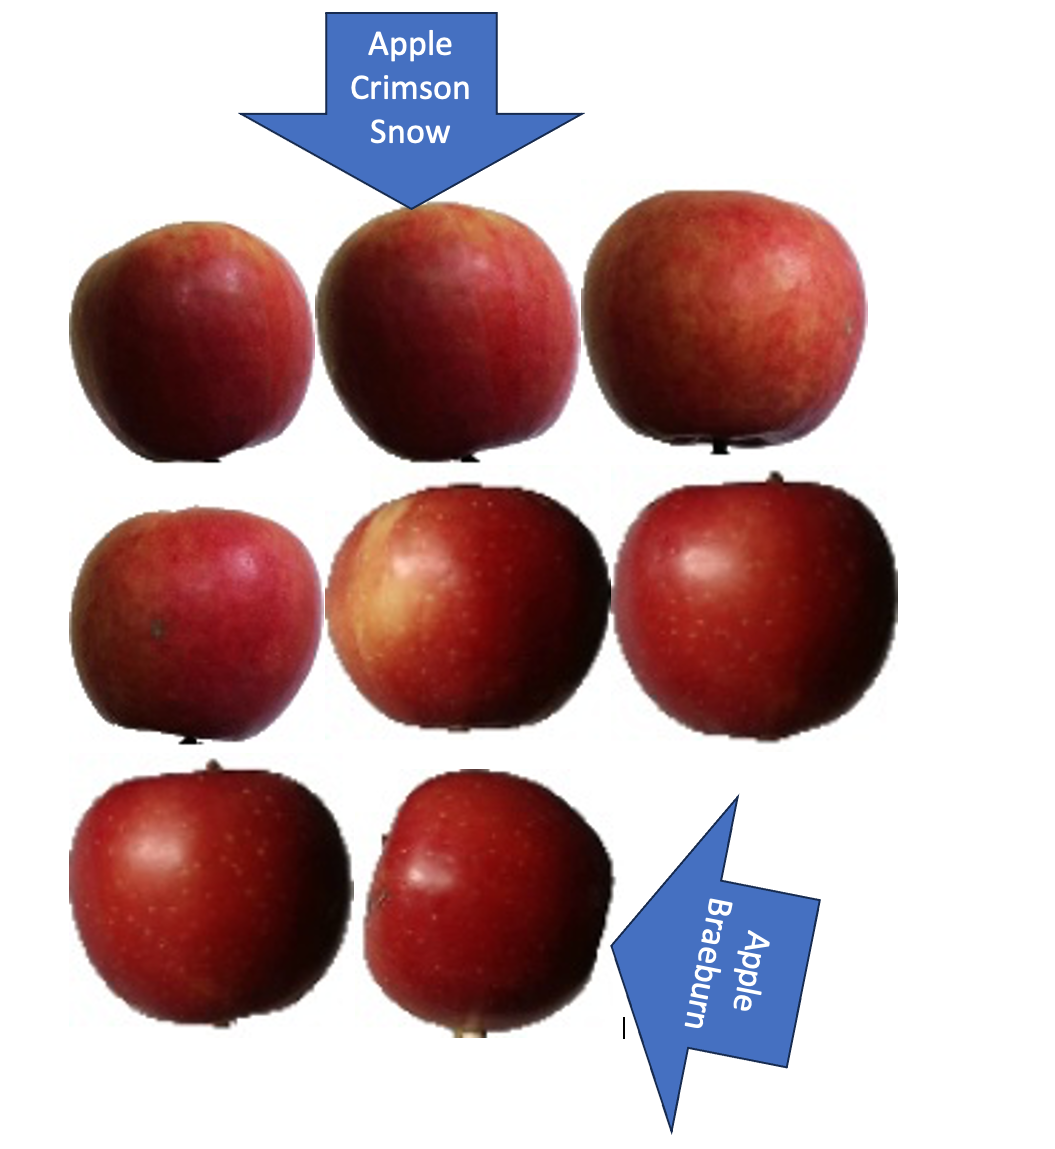
\includegraphics[scale=.35]{Apple-Apple.png} 
   \end{center}
  } \\
  

\end{frame}

\end{document}
